\documentclass[11pt]{article}
\usepackage[utf8]{inputenc}
\usepackage[spanish]{babel}
\decimalpoint
\usepackage{amsmath}
\usepackage{amsthm}
\usepackage{amssymb}
\usepackage{graphicx}
\usepackage[margin=0.8in]{geometry}
\usepackage{fancyhdr}
\usepackage[inline]{enumitem}
\usepackage{float}
\usepackage{cancel}
\usepackage{bigints}
\usepackage{listings}
\usepackage{xcolor}
\usepackage{listingsutf8}
\usepackage{algpseudocode}
\usepackage{algorithm}
\usepackage{apacite}
\usepackage{tcolorbox}
\usepackage{multicol}
\usepackage{tipa}
\usepackage{caption} 
\pagestyle{fancy}
\usepackage{hyperref}
\usepackage{mathtools}% http://ctan.org/pkg/mathtools

\hypersetup{
    colorlinks,
    citecolor=black,
    filecolor=black,
    linkcolor=black,
    urlcolor=black
}
\newcommand{\xvdash}[1]{%
	\vdash^{\mkern-10mu\scriptscriptstyle\rule[-.9ex]{0pt}{0pt}#1}%
}
\setlength{\headheight}{15pt} 
\lhead{Tarea 9. Instalación de NFS en la nube utilizando comunicación segura}
\rhead{\thepage}
\lfoot{ESCOM-IPN}
\renewcommand{\footrulewidth}{0.5pt}
\setlength{\parskip}{0.5em}
\newcommand{\ve}[1]{\overrightarrow{#1}}
\newcommand{\abs}[1]{\left\lvert #1 \right\lvert}
\newcommand{\blank}{\text{\textcrb}}
\date{\today}
\title{Tarea 9. Instalación de NFS en la nube utilizando comunicación segura}
\author{Sanchez Mendez Edmundo Josue}

\lstset{
tabsize = 4, %% set tab space width
showstringspaces = false, %% prevent space marking in strings, string is defined as the text that is generally printed directly to the console
numbers = left, %% display line numbers on the left
commentstyle = \color{green}, %% set comment color
keywordstyle = \color{blue}, %% set keyword color
stringstyle = \color{red}, %% set string color
rulecolor = \color{black}, %% set frame color to avoid being affected by text color
basicstyle = \small \ttfamily , %% set listing font and size
breaklines = true, %% enable line breaking
numberstyle = \tiny,
}

\bibliographystyle{apacite}
\begin{document}
		\begin{titlepage}
			\begin{center}
				
				% Upper part of the page. The '~' is needed because \\
				% only works if a paragraph has started.
				
				\noindent
				\begin{minipage}{0.5\textwidth}
					\begin{flushleft} \large
						
\includegraphics[width=0.5\textwidth]{resources/ipn.png}
					\end{flushleft}
				\end{minipage}%
				\begin{minipage}{0.55\textwidth}
					\begin{flushright} \large
						
\includegraphics[width=0.5\textwidth]{resources/escom.png}
					\end{flushright}
				\end{minipage}
				
				\textsc{\LARGE Instituto Politécnico Nacional}\\[0.5cm]
				
				\textsc{\Large Escuela Superior de Cómputo}\\[1cm]
				
				% Title
				
				{ \huge Tarea 9. Instalación de NFS en la nube utilizando comunicación segura \\[1cm] }
				
				{ \Large Unidad de aprendizaje: Desarrollo de Sistemas Distribuidos} \\[1cm]
				
				{ \Large Grupo: 4CV11 } \\[1cm]
				
				\noindent
				\begin{minipage}{0.5\textwidth}
					\begin{flushleft} \large
						\emph{Alumno:} \\
						Sanchez Mendez Edmundo Josue
					\end{flushleft}
				\end{minipage}%
				\begin{minipage}{0.5\textwidth}
					\begin{flushright} \large
						\emph{Profesor:} \\
						Pineda Guerrero Carlos 
					\end{flushright}
				\end{minipage}
				
				\vfill
				% Bottom of the page
				{\large {\today}}
			\end{center}
		\end{titlepage}
	
	\titlepage
	\tableofcontents
	\newpage
	
	\section{Introducción}
	Tomando como base la actividad que realizamos en clase, dónde instalamos NFS en dos máquinas virtuales en la nube, realizar el siguiente procedimiento:
		\begin{enumerate}
			\item Crear tres máquinas virtuales con \textbf{Ubuntu 18 en la nube de Azure.}
			\item En una máquina virtual instalar un servidor NFS y en dos máquinas virtuales instalar clientes NFS.
			\item Crear en el servidor el directorio (punto de montaje del servidor): /var/servidor
			\item Crear en cada cliente el directorio (punto de montaje en el cliente): /cliente
			\item En el cliente 1 crear un archivo de texto llamado ``archivo.txt'' en el directorio /cliente
			\item Agregar al archivo ``archivo.txt'' el texto ``esta es una prueba de NFS'' y guardar el archivo.
			\item En el cliente 2 desplegar el contenido del archivo /cliente/archivo.txt utilizando el comando ``more''
			\item Configurar cada cliente para que inicie NFS al momento encender la computadora.
			\item Apagar y encender cada cliente.
			\item En el cliente 1 desplegar el archivo /cliente/archivo.txt utilizando el comando ``more''
			\item En el cliente 2 desplegar el archivo /cliente/archivo.txt utilizando el comando ``more''
			\item En el cliente 2 modificar el archivo /cliente/archivo.txt, agregar al archivo el siguiente texto: ``estamos agregando texto al archivo''
			\item En el cliente 1 desplegar el archivo /cliente/archivo.txt utilizando el comando ``more''
			\item En el cliente 1 eliminar el archivo /cliente/archivo.txt utilizando el comando ``rm''
			\item En el cliente 1 desplegar el contenido del directorio /cliente utilizando el comando ``ls''
			\item En el cliente 2 desplegar el contenido del directorio /cliente utilizando el comando ``ls''
		\end{enumerate}
		
	\section{Desarrollo}
		\subsection{Creación de la maquina virtual para el servidor}
En esta parte veremos la creación de la maquina virtual la cual funcionara como nuestro servidor para el desarrollo de esta practica.
		\begin{figure}[H]
			\centering
			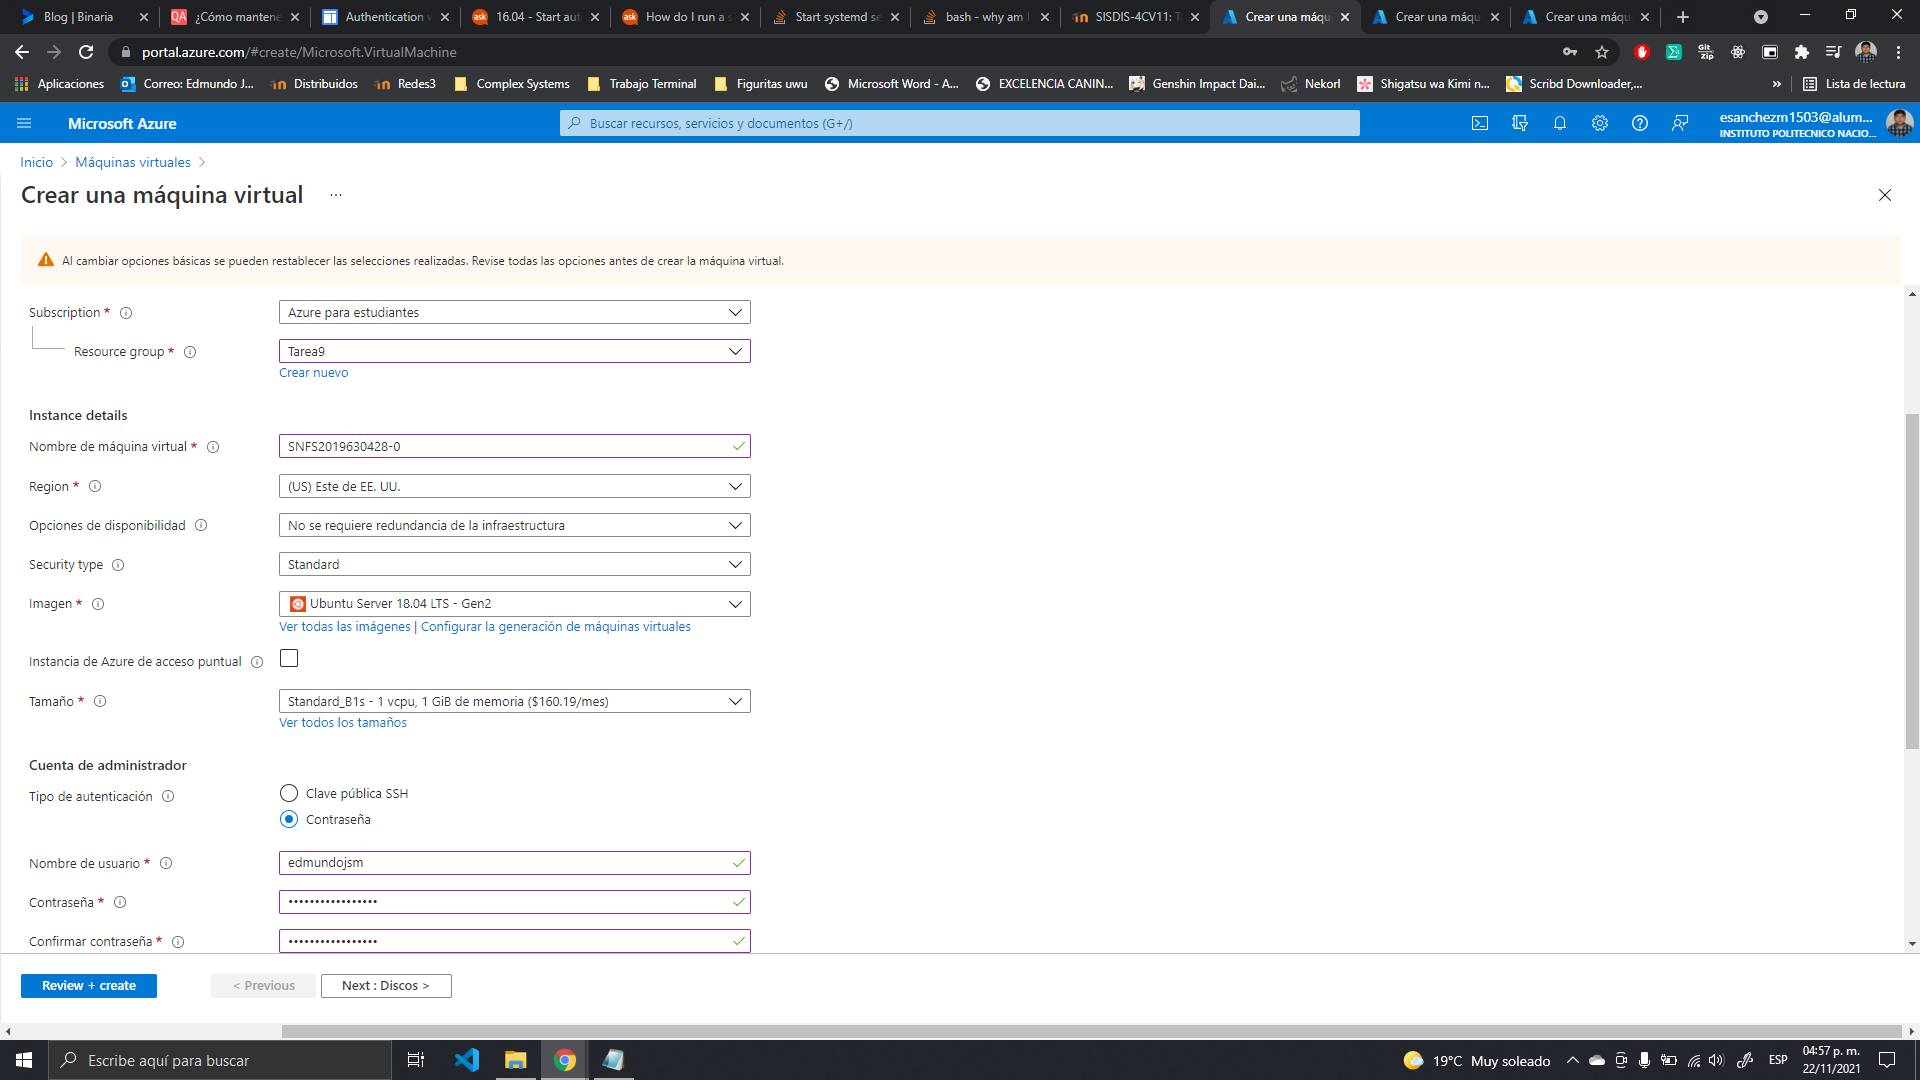
\includegraphics[scale=0.34]{resources/Infobasica0.png}
			\caption{Datos básicos de la maquina virtual.}\label{fig:picture}
		\end{figure}
		\begin{figure}[H]
			\centering
			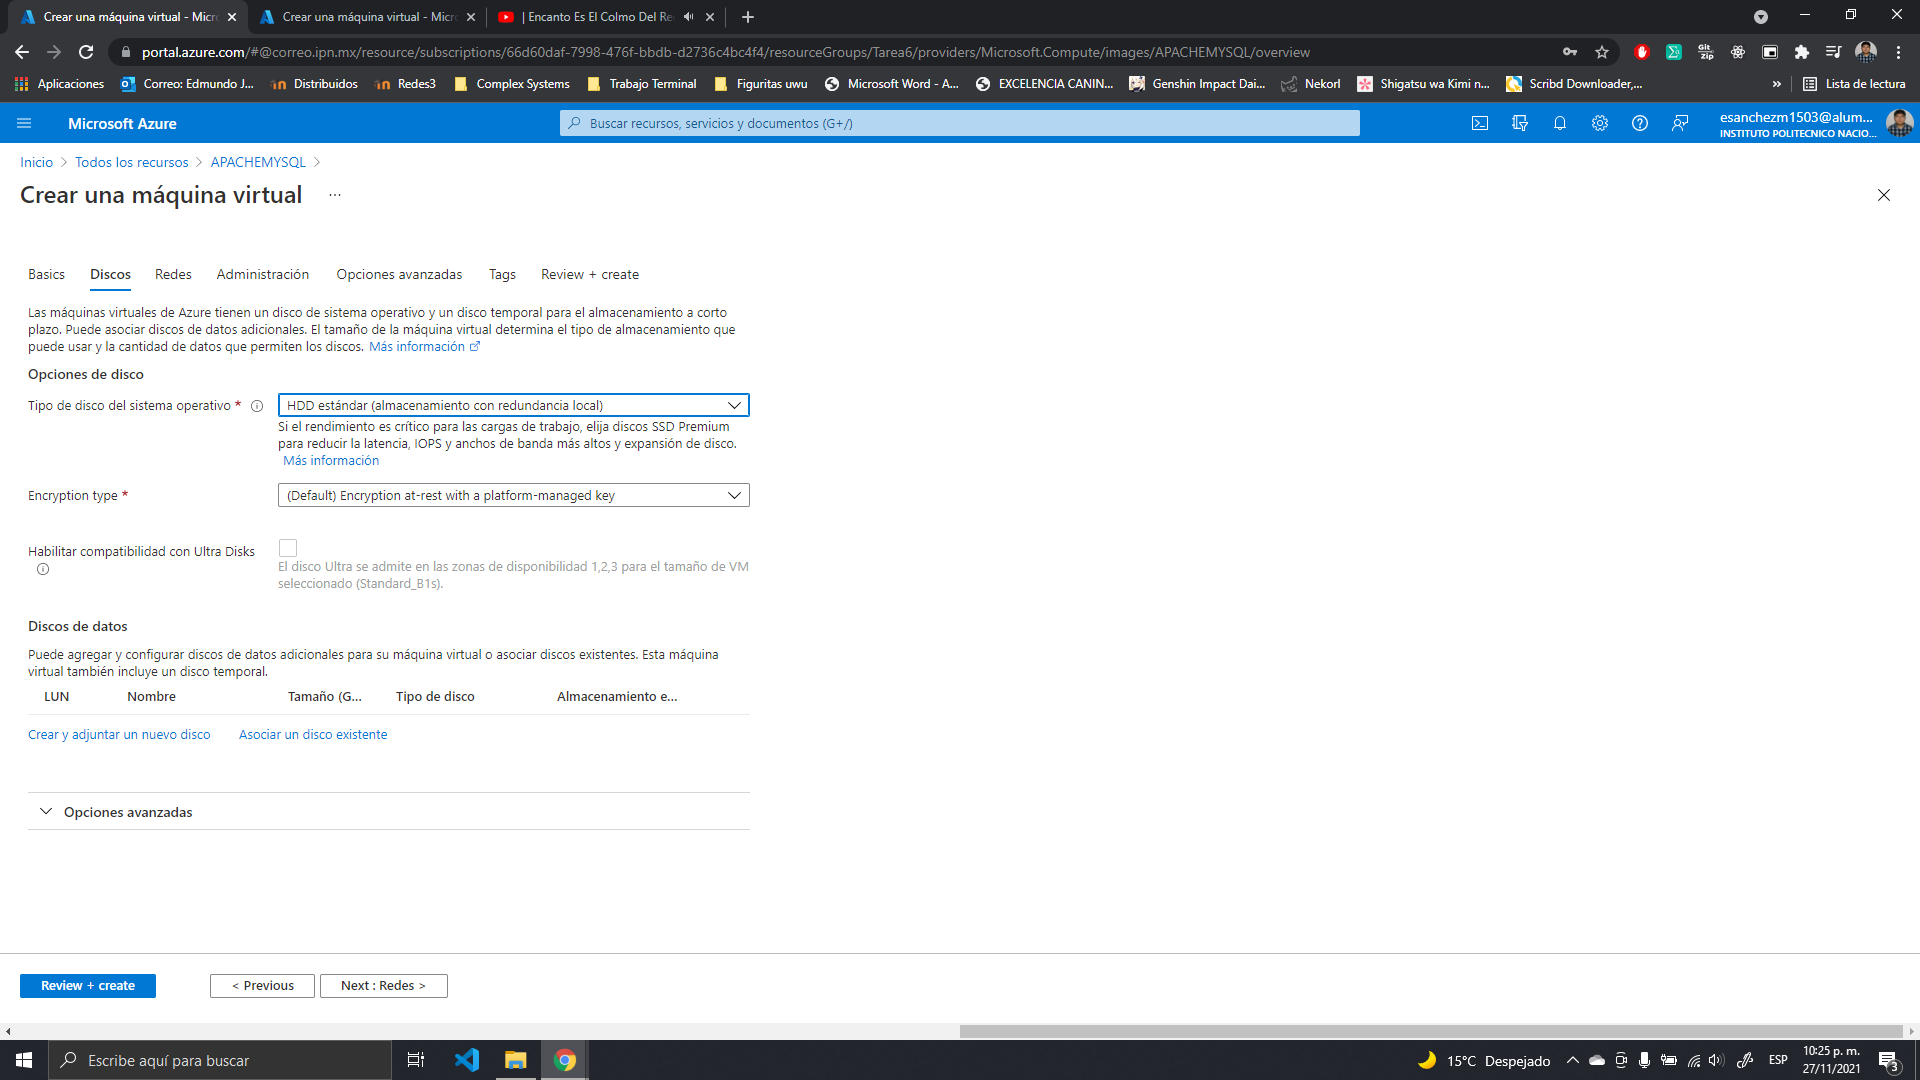
\includegraphics[scale=0.34]{resources/disco0.png}
			\caption{Configuración del tipo de disco de la maquina virtual.}\label{fig:picture}
		\end{figure}
		\begin{figure}[H]
			\centering
			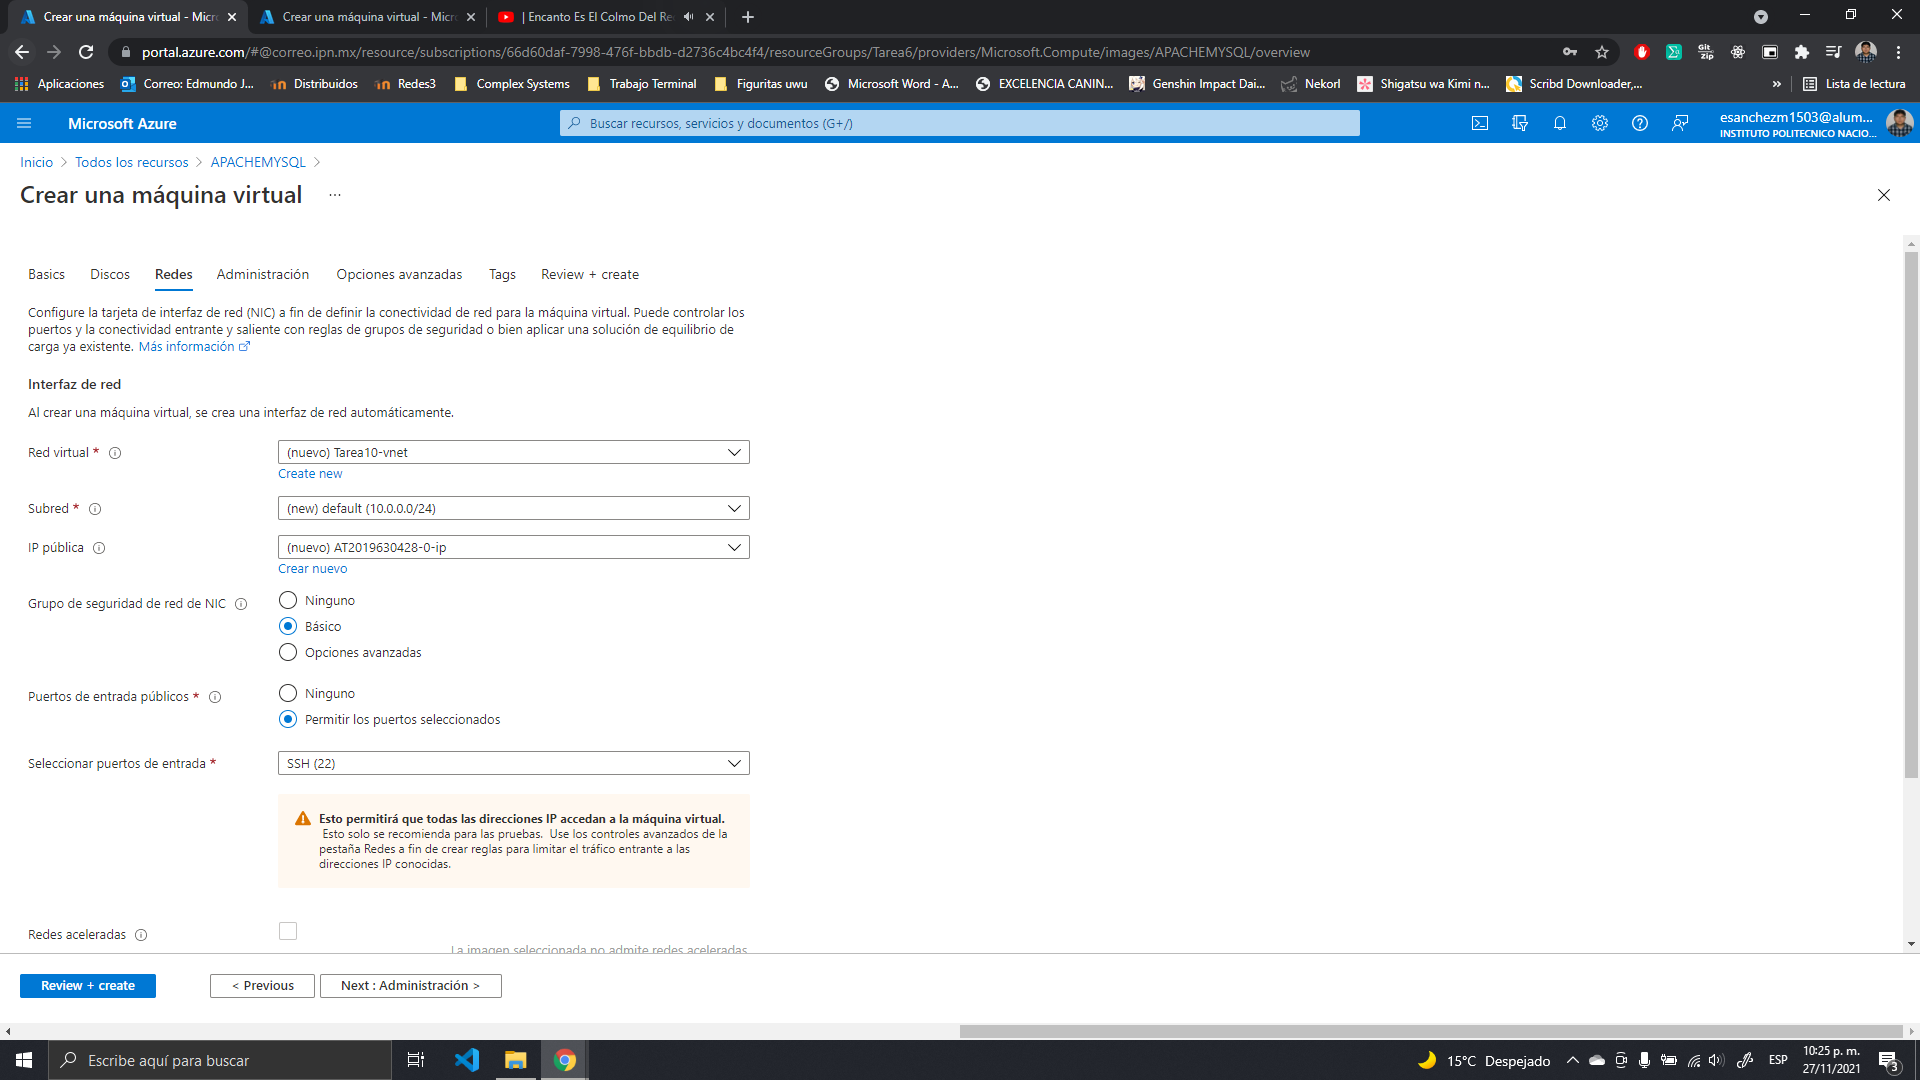
\includegraphics[scale=0.34]{resources/redes0.png}
			\caption{Información sobre la redes de la maquina virtual.}\label{fig:picture}
		\end{figure}
		\begin{figure}[H]
			\centering
			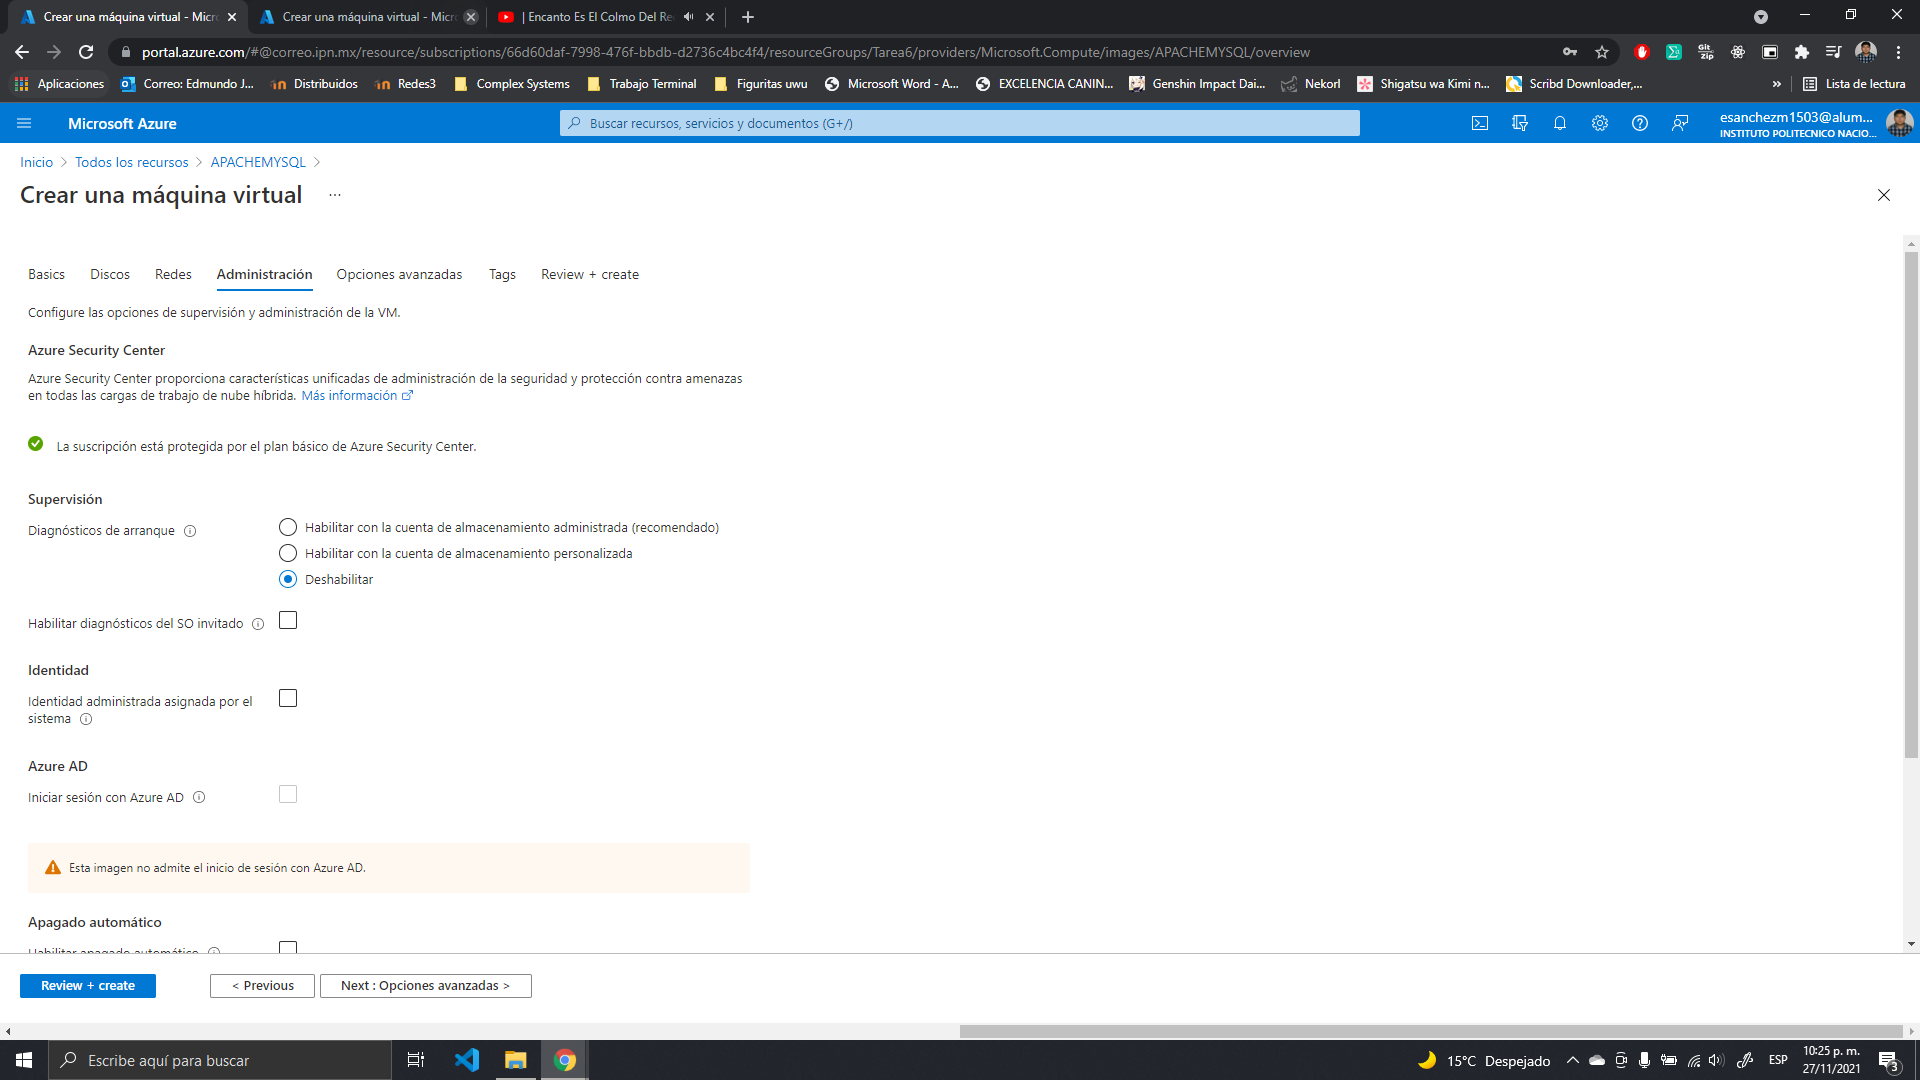
\includegraphics[scale=0.34]{resources/admin0.png}
			\caption{Configuración de la administración de la maquina virtual.}\label{fig:picture}
		\end{figure}
		\begin{figure}[H]
			\centering
			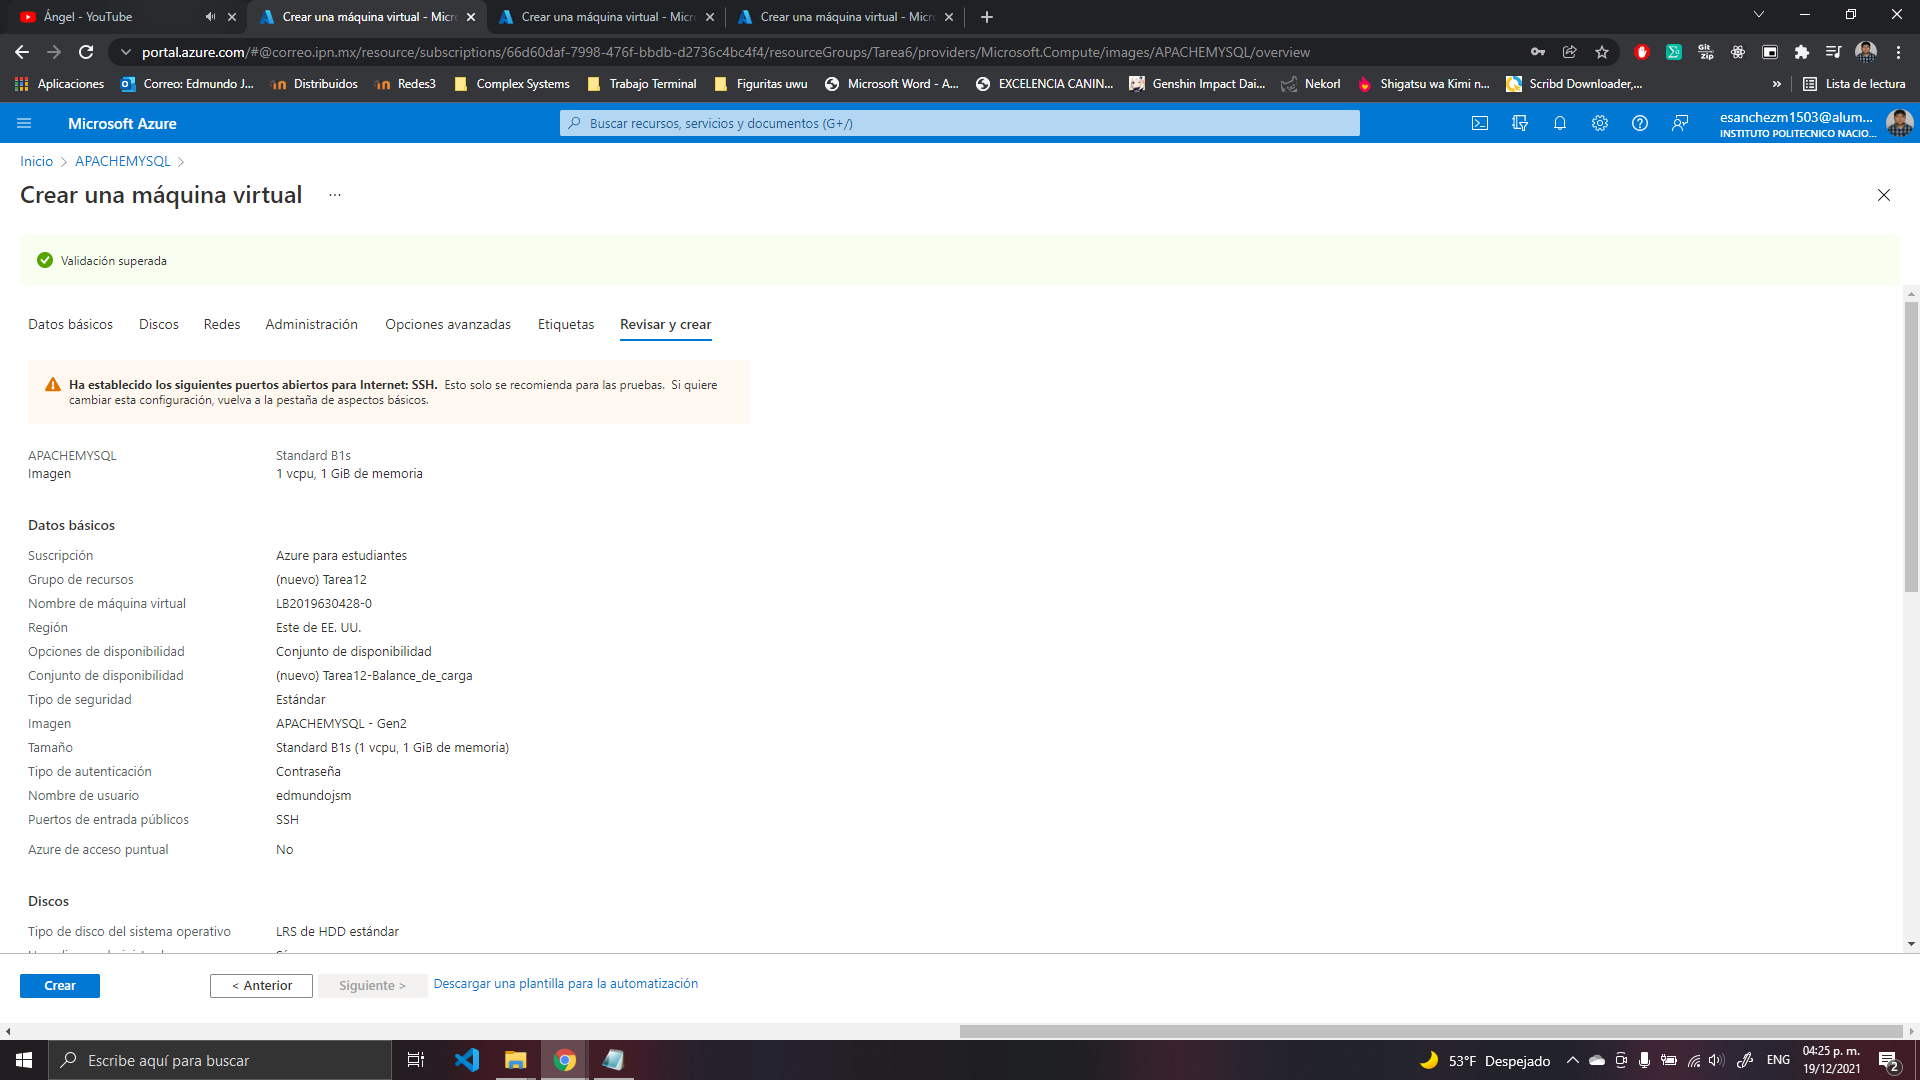
\includegraphics[scale=0.34]{resources/revisarycrear0.png}
			\caption{Creación de la maquina virtual.}\label{fig:picture}
		\end{figure}
		\begin{figure}[H]
			\centering
			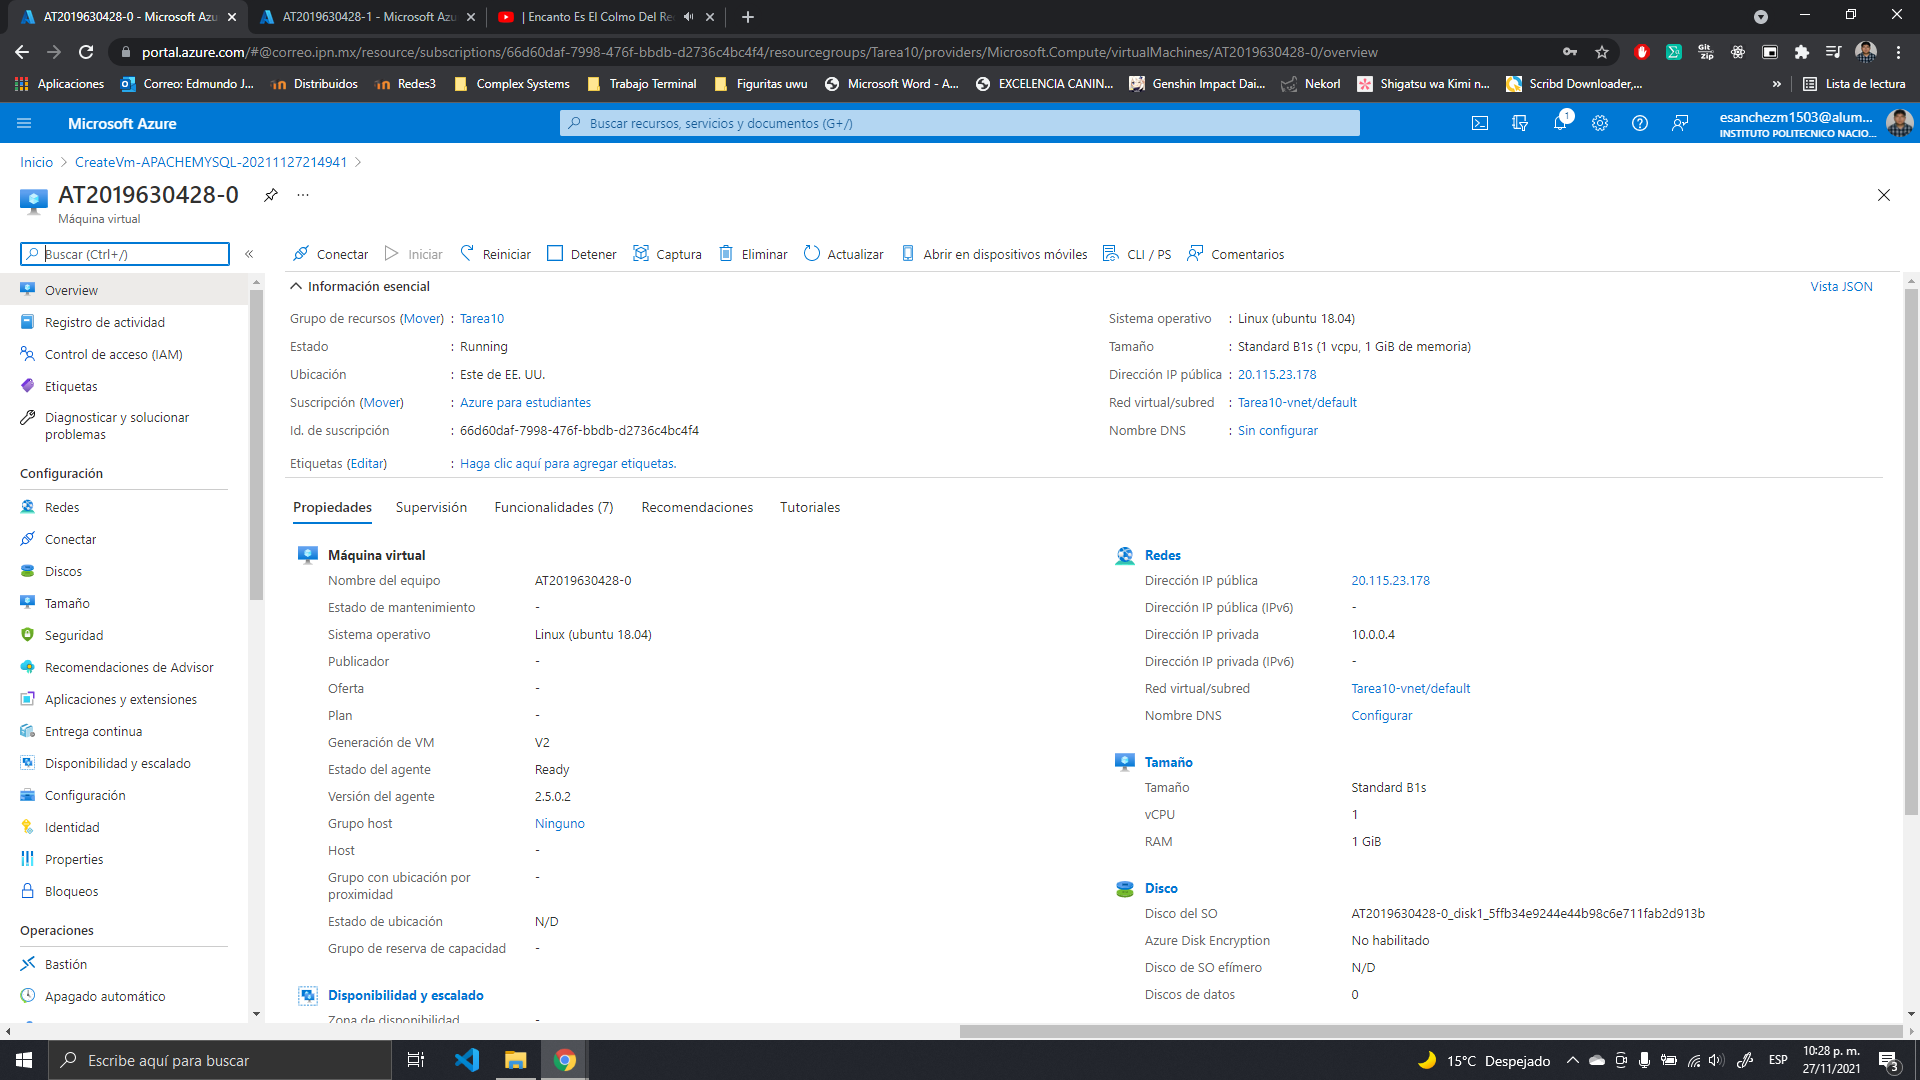
\includegraphics[scale=0.34]{resources/paneldecontrol0.png}
			\caption{Panel de control de la maquina virtual.}\label{fig:picture}
		\end{figure}
		Una vez creada la maquina virtual tenemos que abrir el puerto 2049, ya que este puerto es el que ocuparemos para NFS. En las figuras 7 y 8 podemos ver la configuración del puerto.
		\begin{figure}[H]
			\centering
			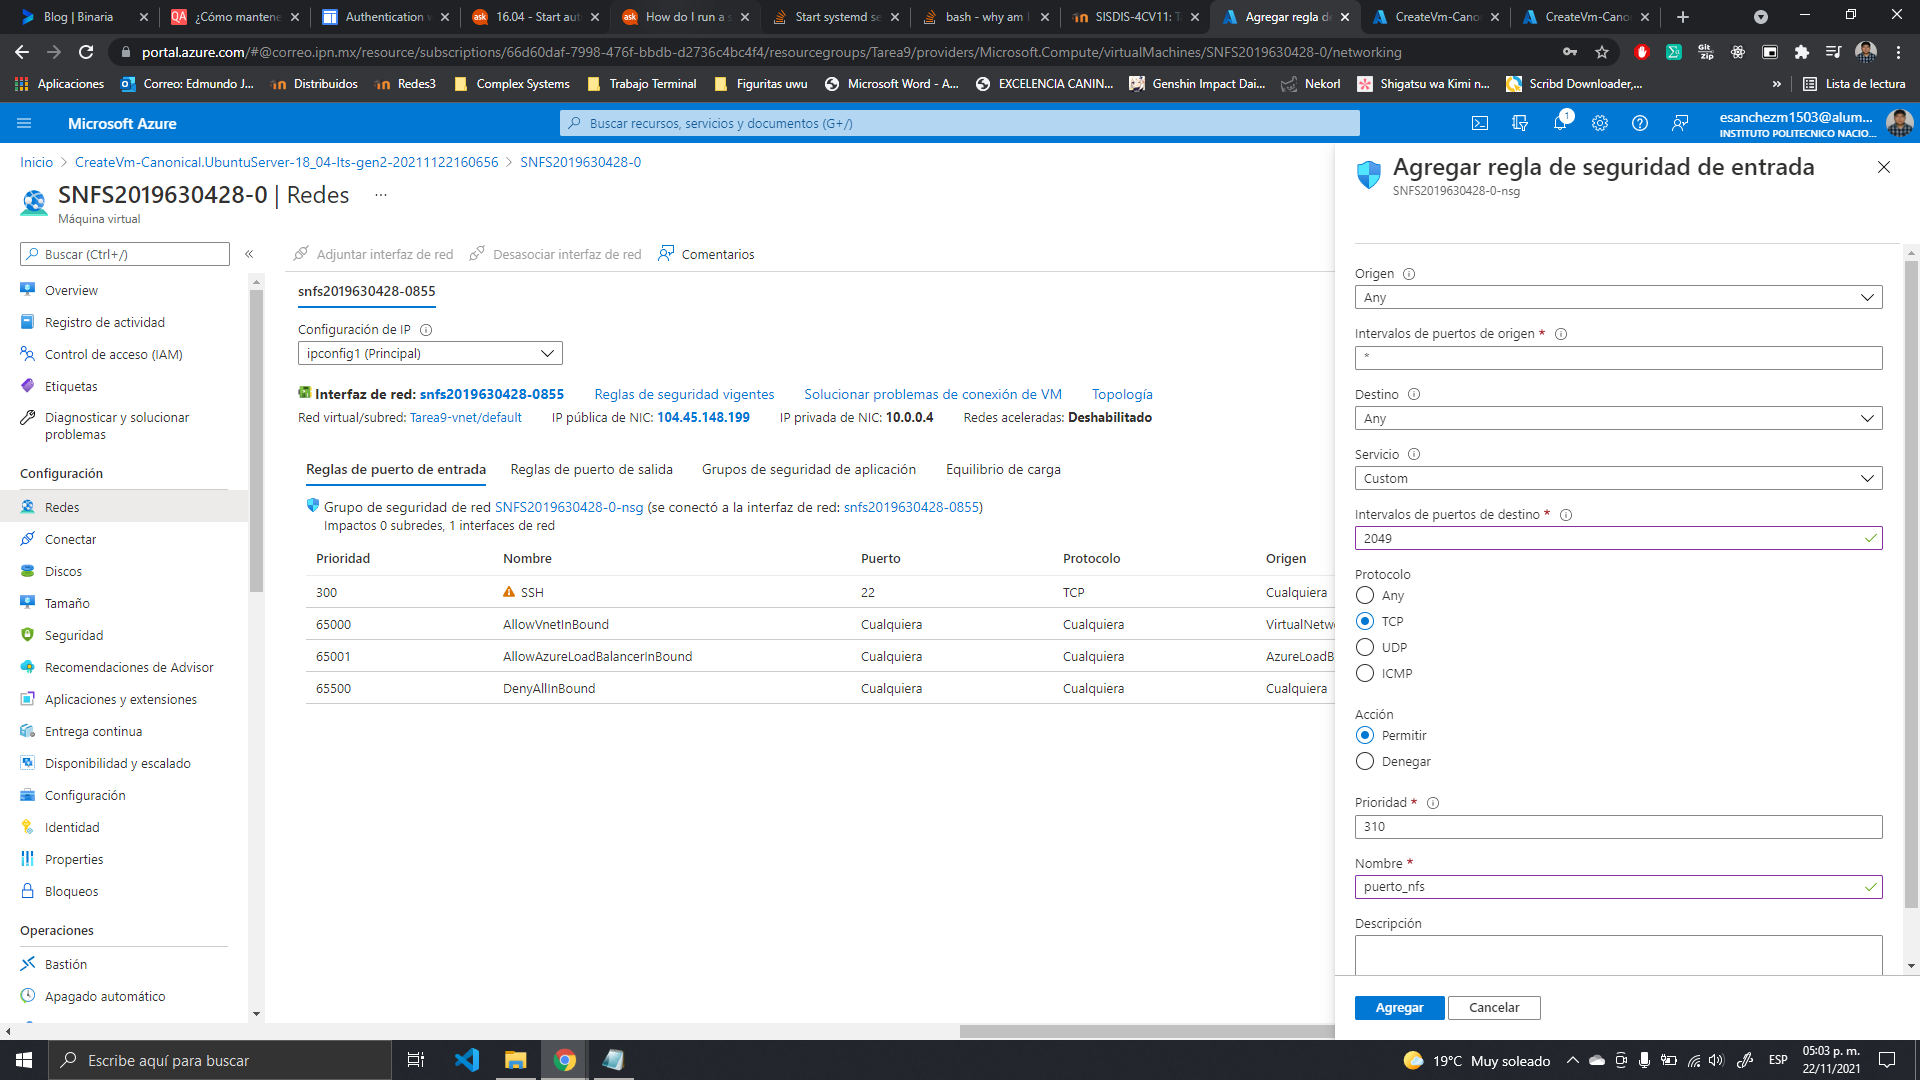
\includegraphics[scale=0.34]{resources/open20490.png}
			\caption{Configuración del puerto 2049.}\label{fig:picture}
		\end{figure}
		\begin{figure}[H]
			\centering
			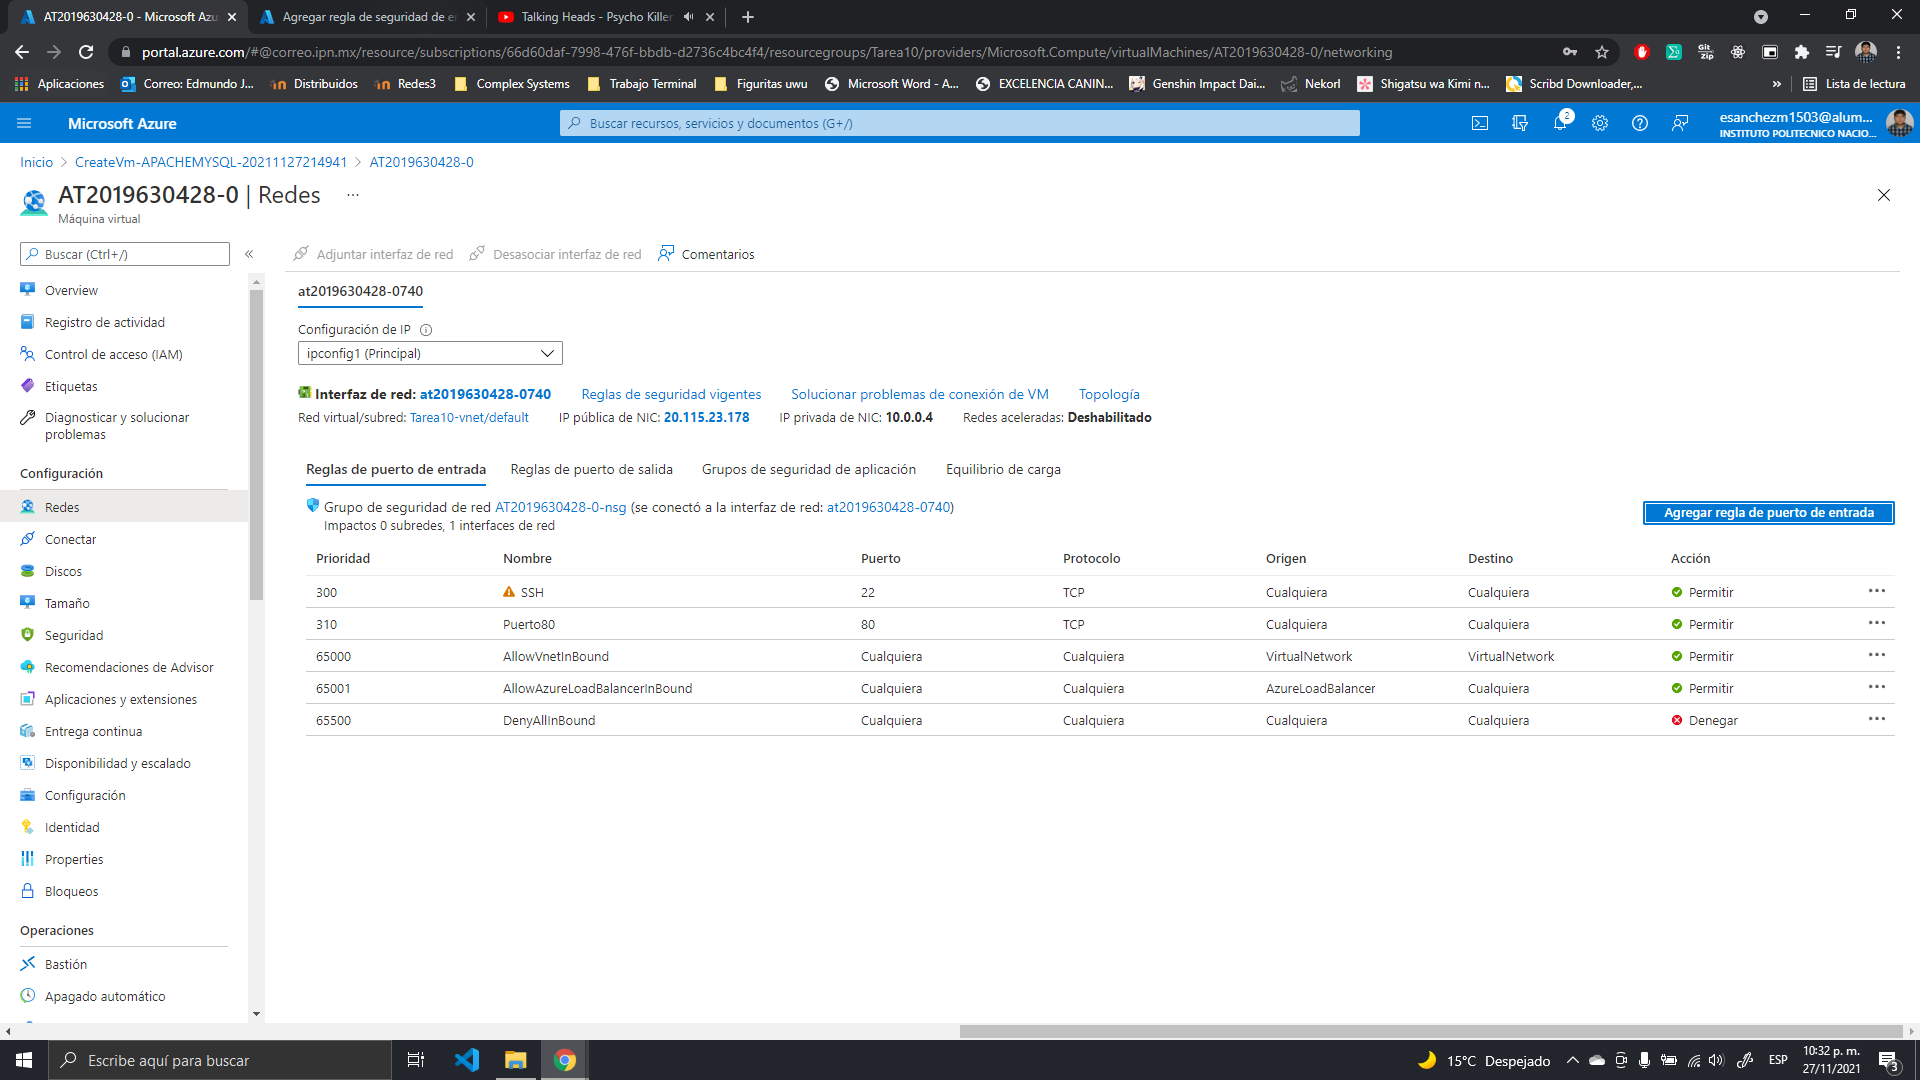
\includegraphics[scale=0.34]{resources/puertook0.png}
			\caption{Puerto 2049 abierto correctamente.}\label{fig:picture}
		\end{figure}
		\subsection{Creación de la maquina virtual para el cliente 1}
En esta parte veremos la creación de la maquina virtual la cual funcionara como nuestro cliente 1 para el desarrollo de esta practica.
		\begin{figure}[H]
			\centering
			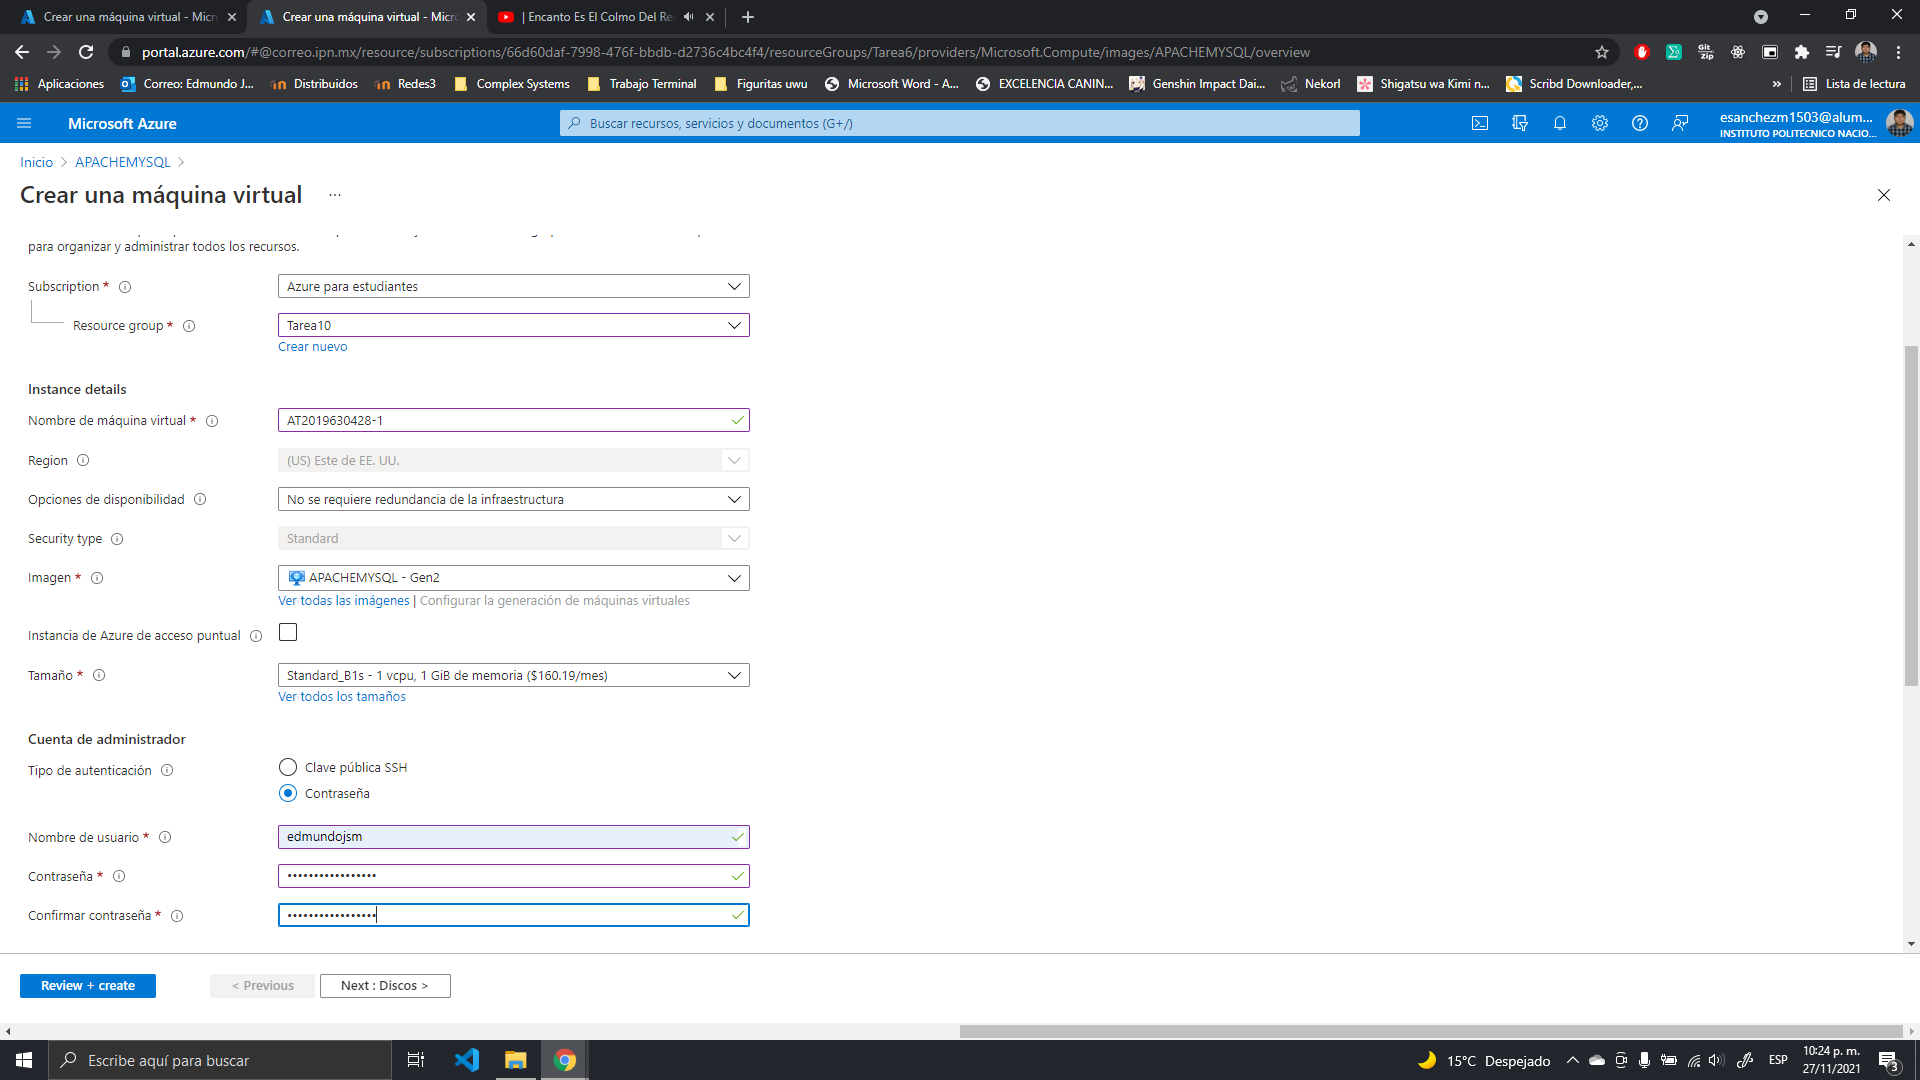
\includegraphics[scale=0.34]{resources/Infobasica1.png}
			\caption{Datos básicos de la maquina virtual.}\label{fig:picture}
		\end{figure}
		\begin{figure}[H]
			\centering
			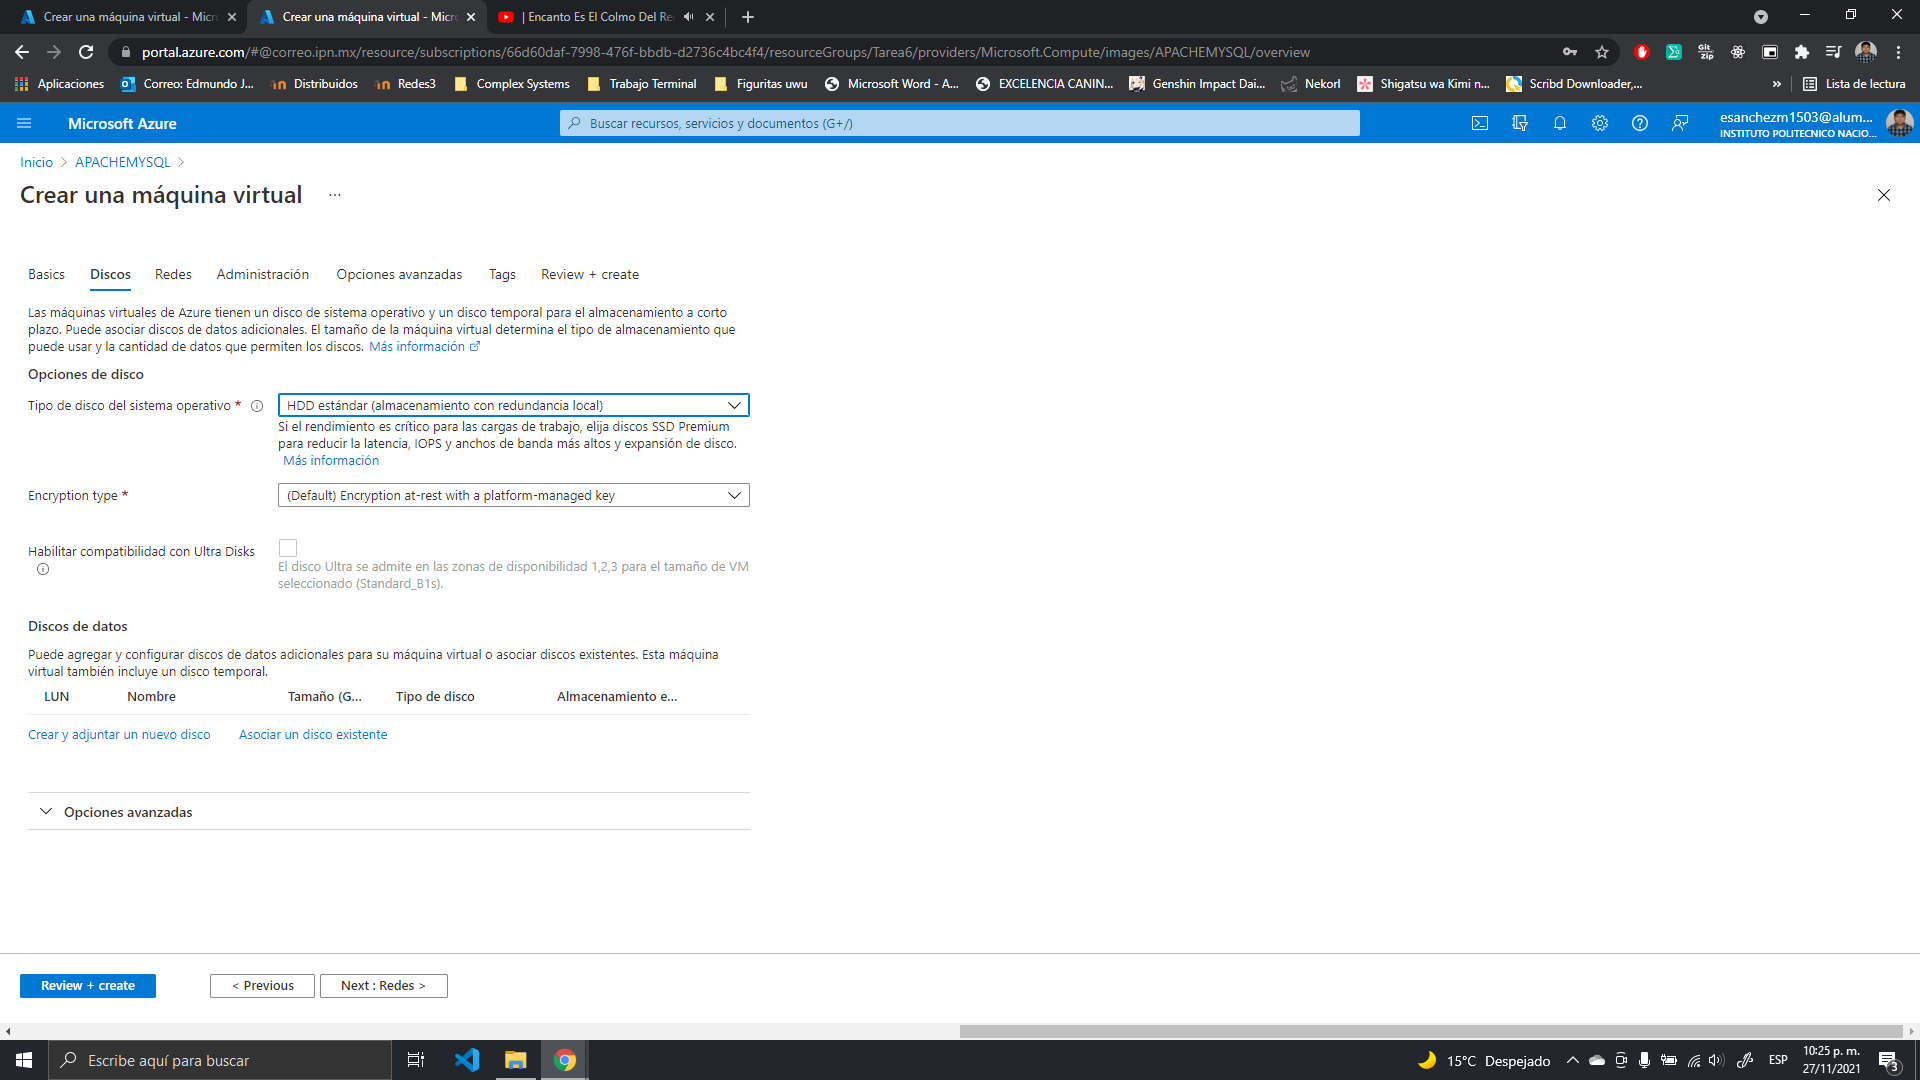
\includegraphics[scale=0.34]{resources/disco1.png}
			\caption{Configuración del tipo de disco de la maquina virtual.}\label{fig:picture}
		\end{figure}
		\begin{figure}[H]
			\centering
			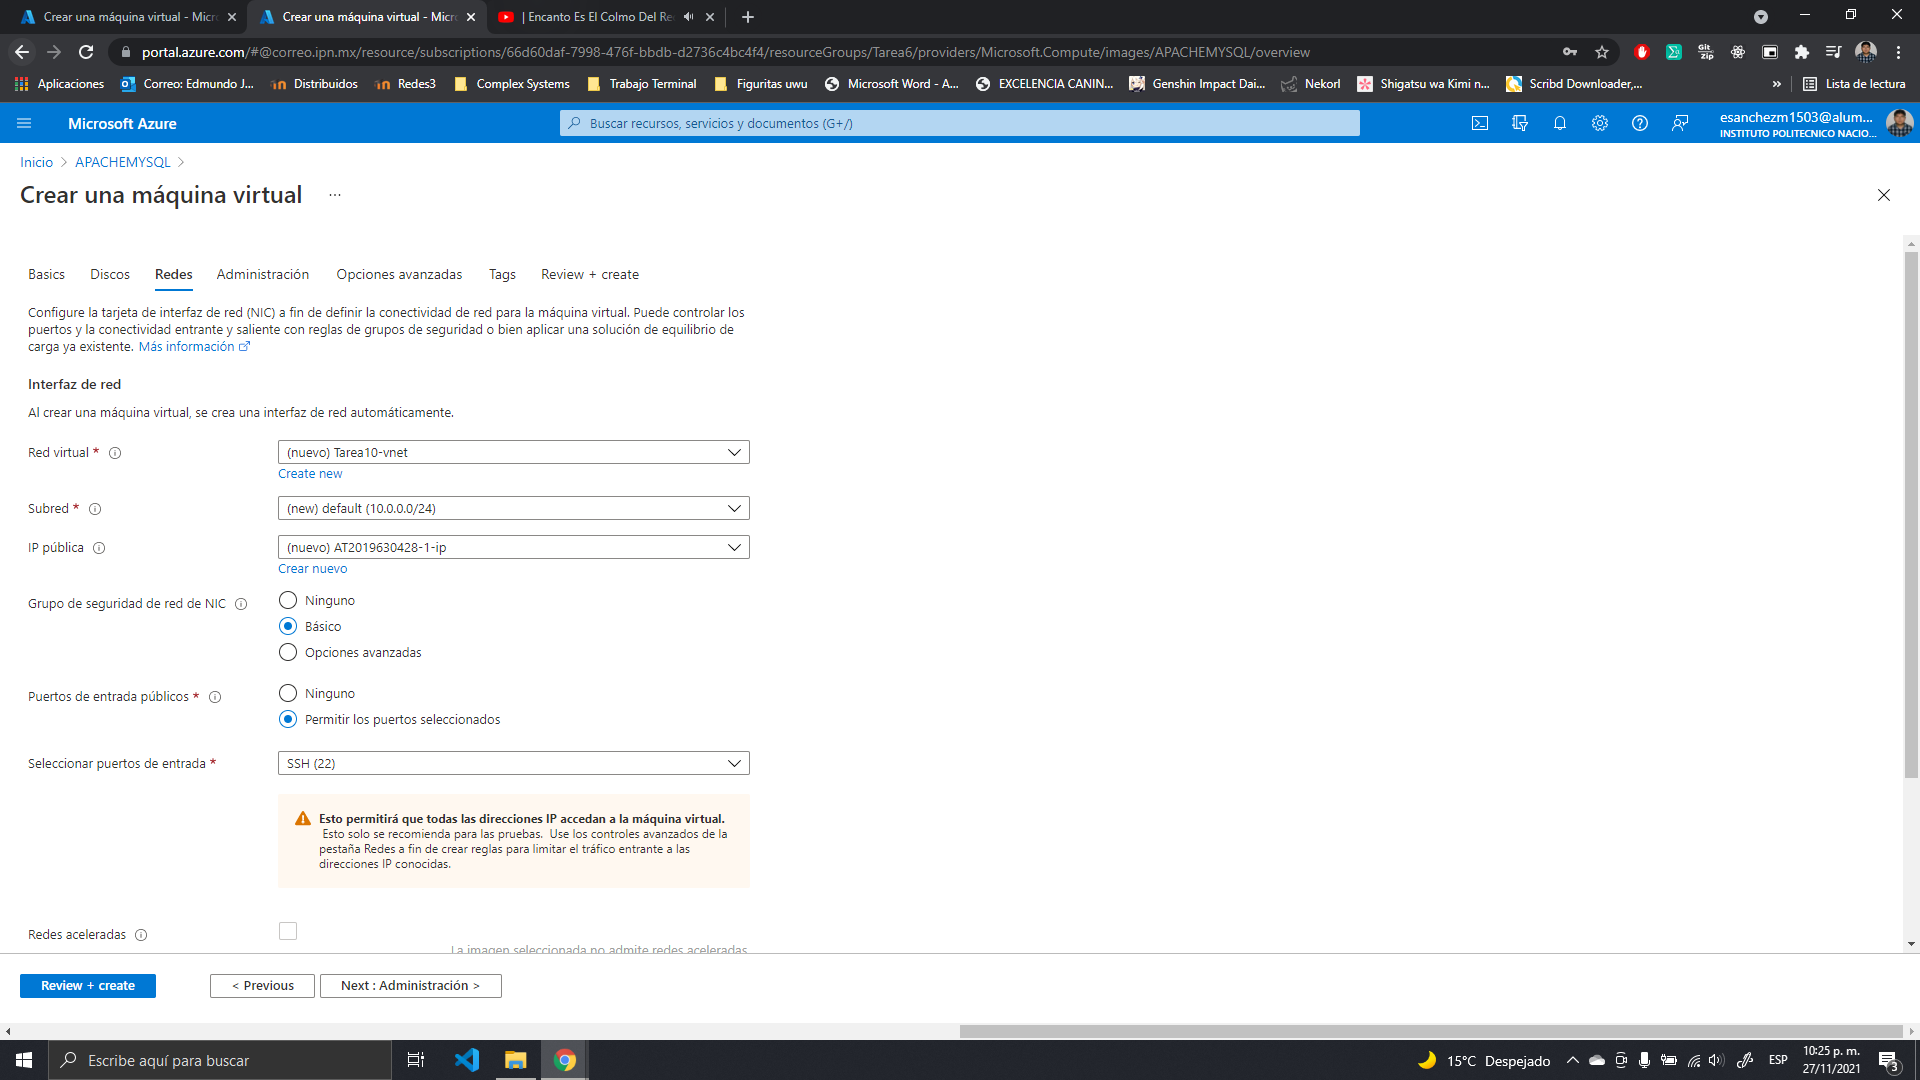
\includegraphics[scale=0.34]{resources/redes1.png}
			\caption{Información sobre la redes de la maquina virtual.}\label{fig:picture}
		\end{figure}
		\begin{figure}[H]
			\centering
			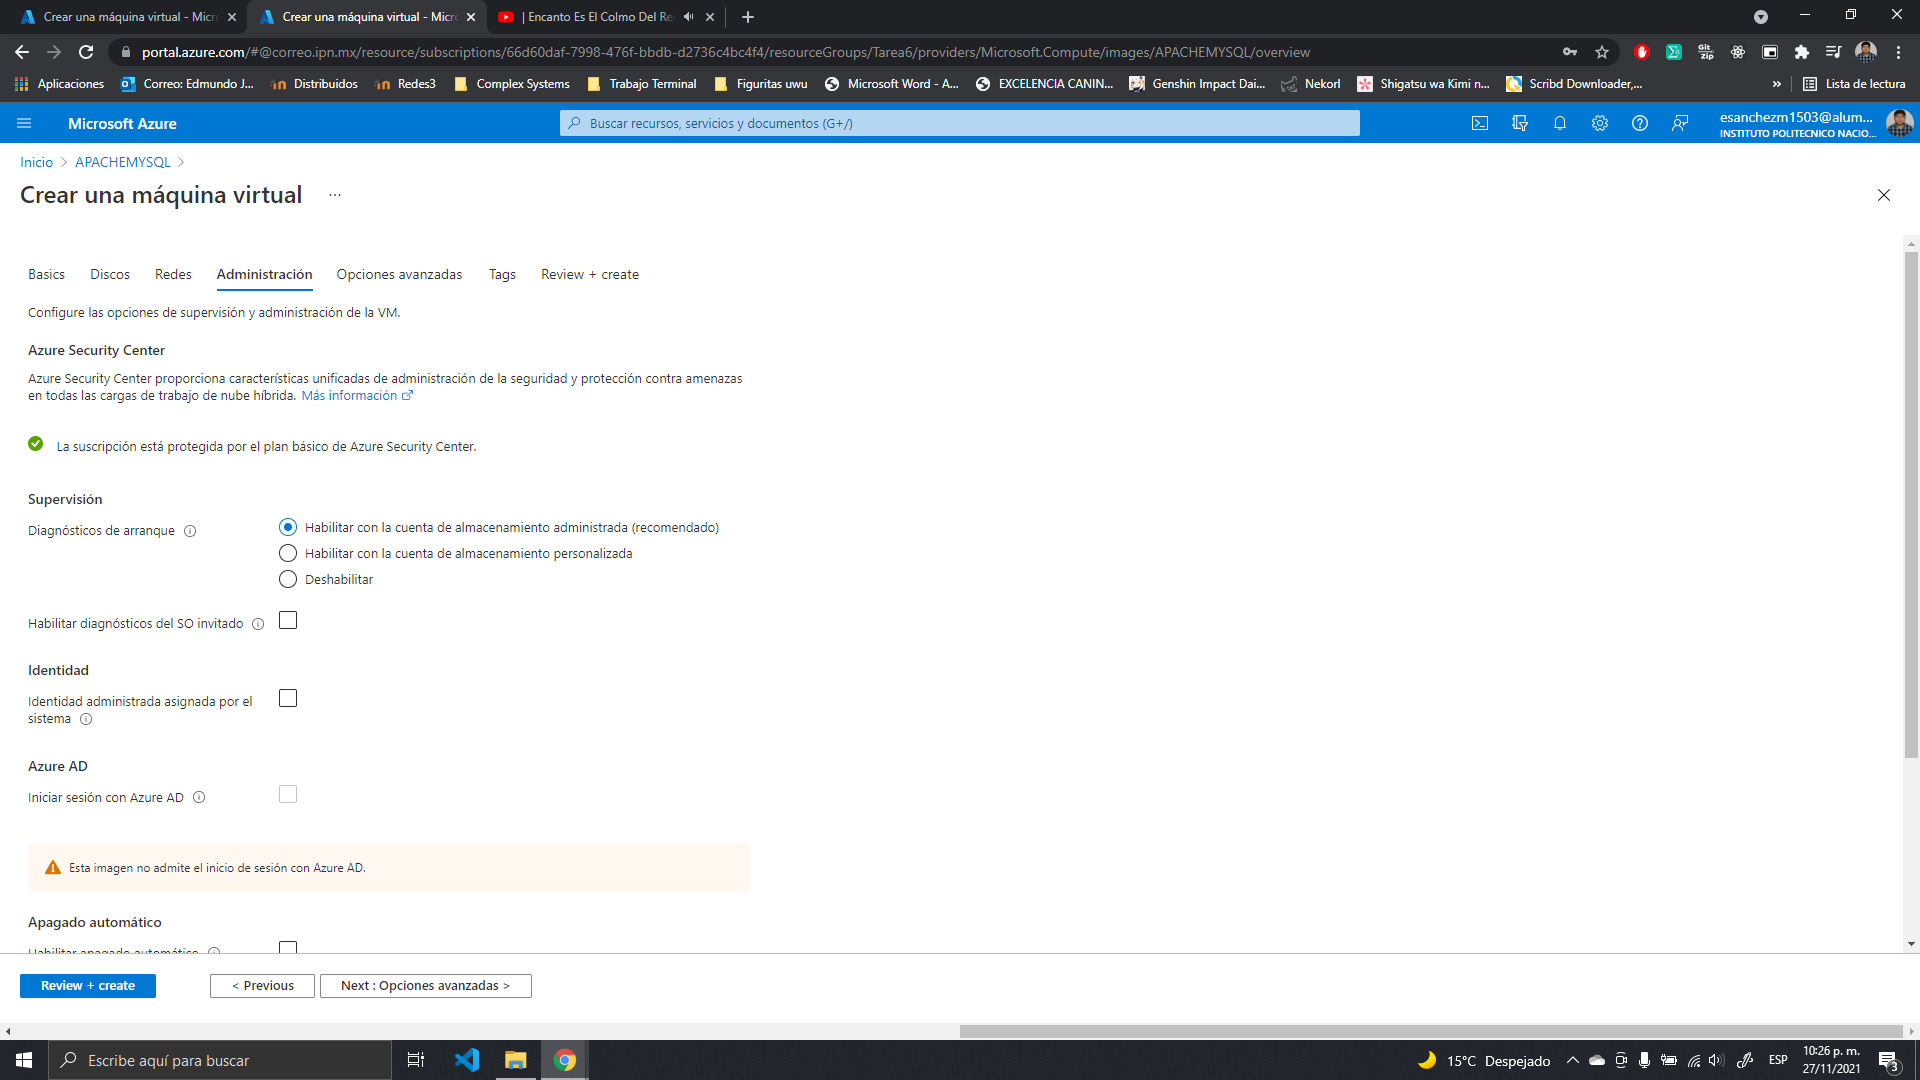
\includegraphics[scale=0.34]{resources/admin1.png}
			\caption{Configuración de la administración de la maquina virtual.}\label{fig:picture}
		\end{figure}
		\begin{figure}[H]
			\centering
			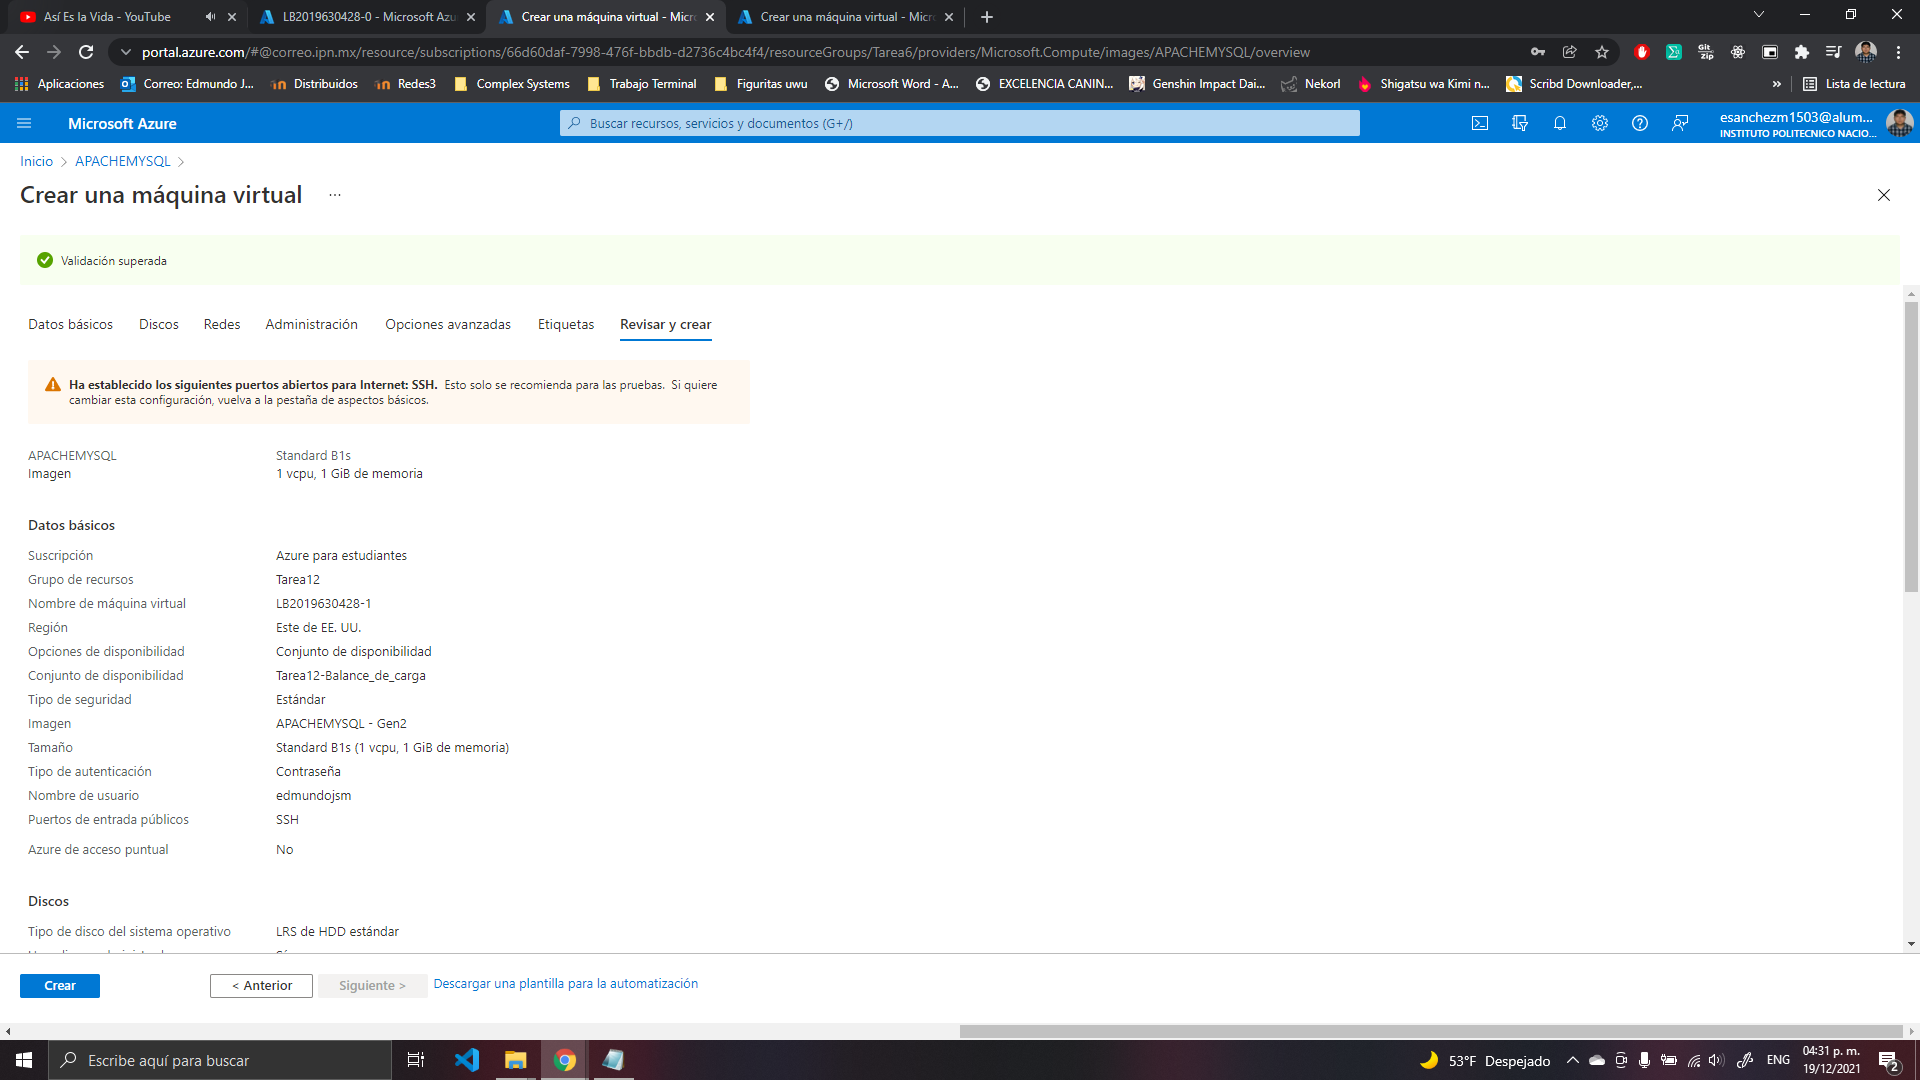
\includegraphics[scale=0.34]{resources/revisarycrear1.png}
			\caption{Creación de la maquina virtual.}\label{fig:picture}
		\end{figure}
		\begin{figure}[H]
			\centering
			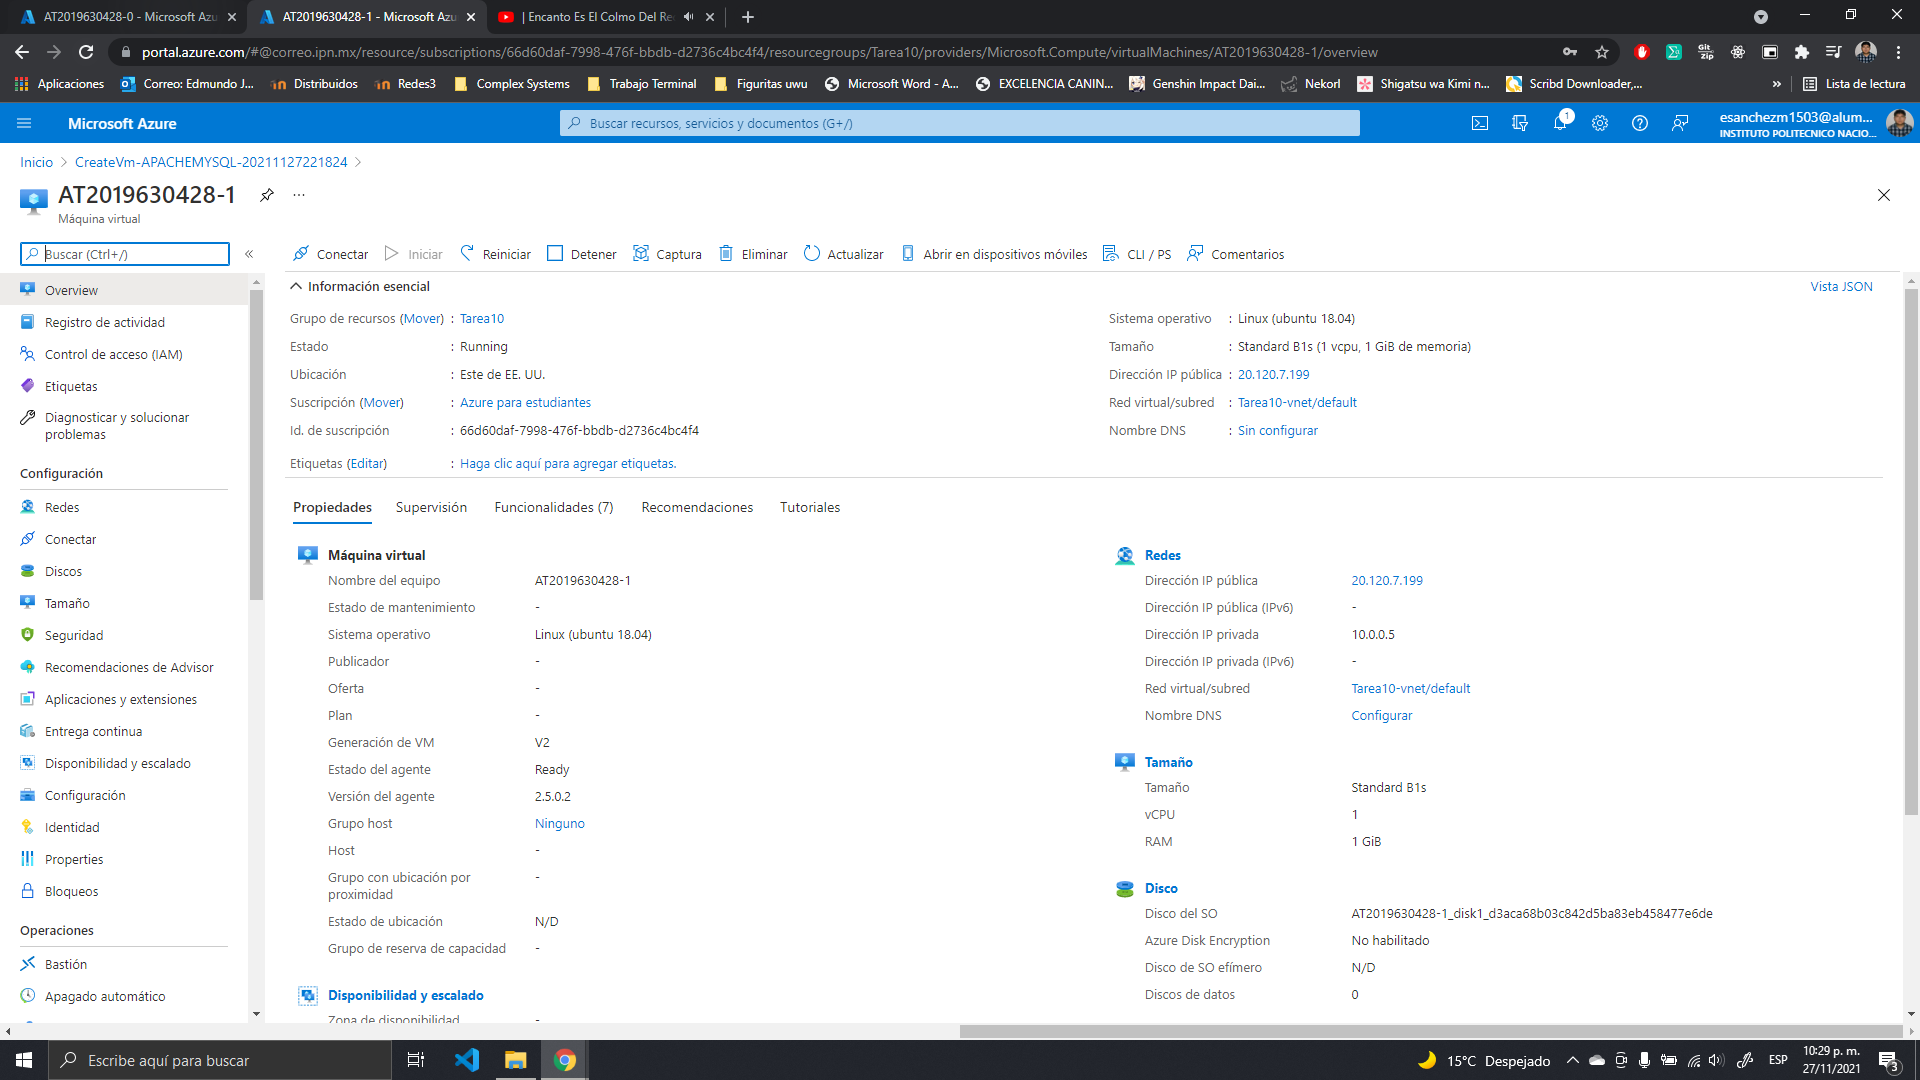
\includegraphics[scale=0.34]{resources/paneldecontrol1.png}
			\caption{Panel de control de la maquina virtual.}\label{fig:picture}
		\end{figure}
		
		\subsection{Creación de la maquina virtual para el cliente 2}
En esta parte veremos la creación de la maquina virtual la cual funcionara como nuestro cliente 2 para el desarrollo de esta practica.
		\begin{figure}[H]
			\centering
			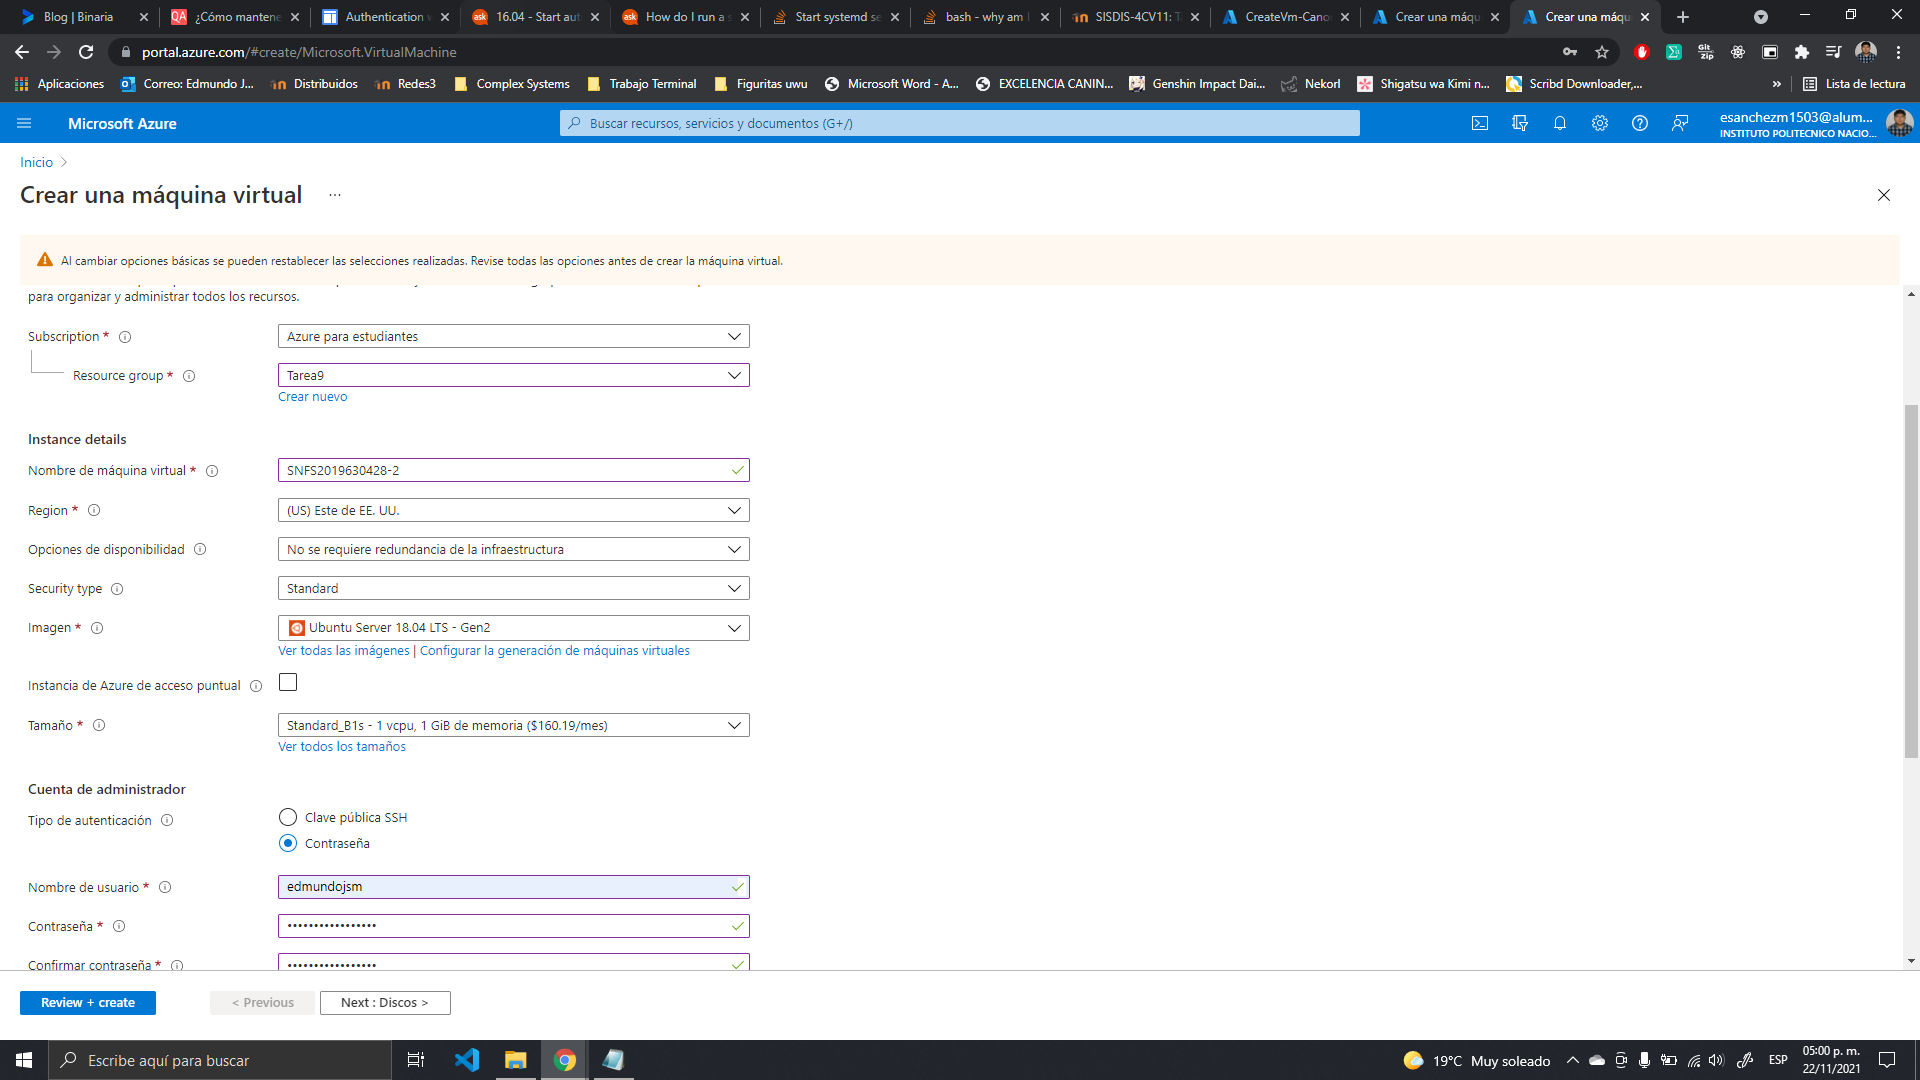
\includegraphics[scale=0.34]{resources/Infobasica2.png}
			\caption{Datos básicos de la maquina virtual.}\label{fig:picture}
		\end{figure}
		\begin{figure}[H]
			\centering
			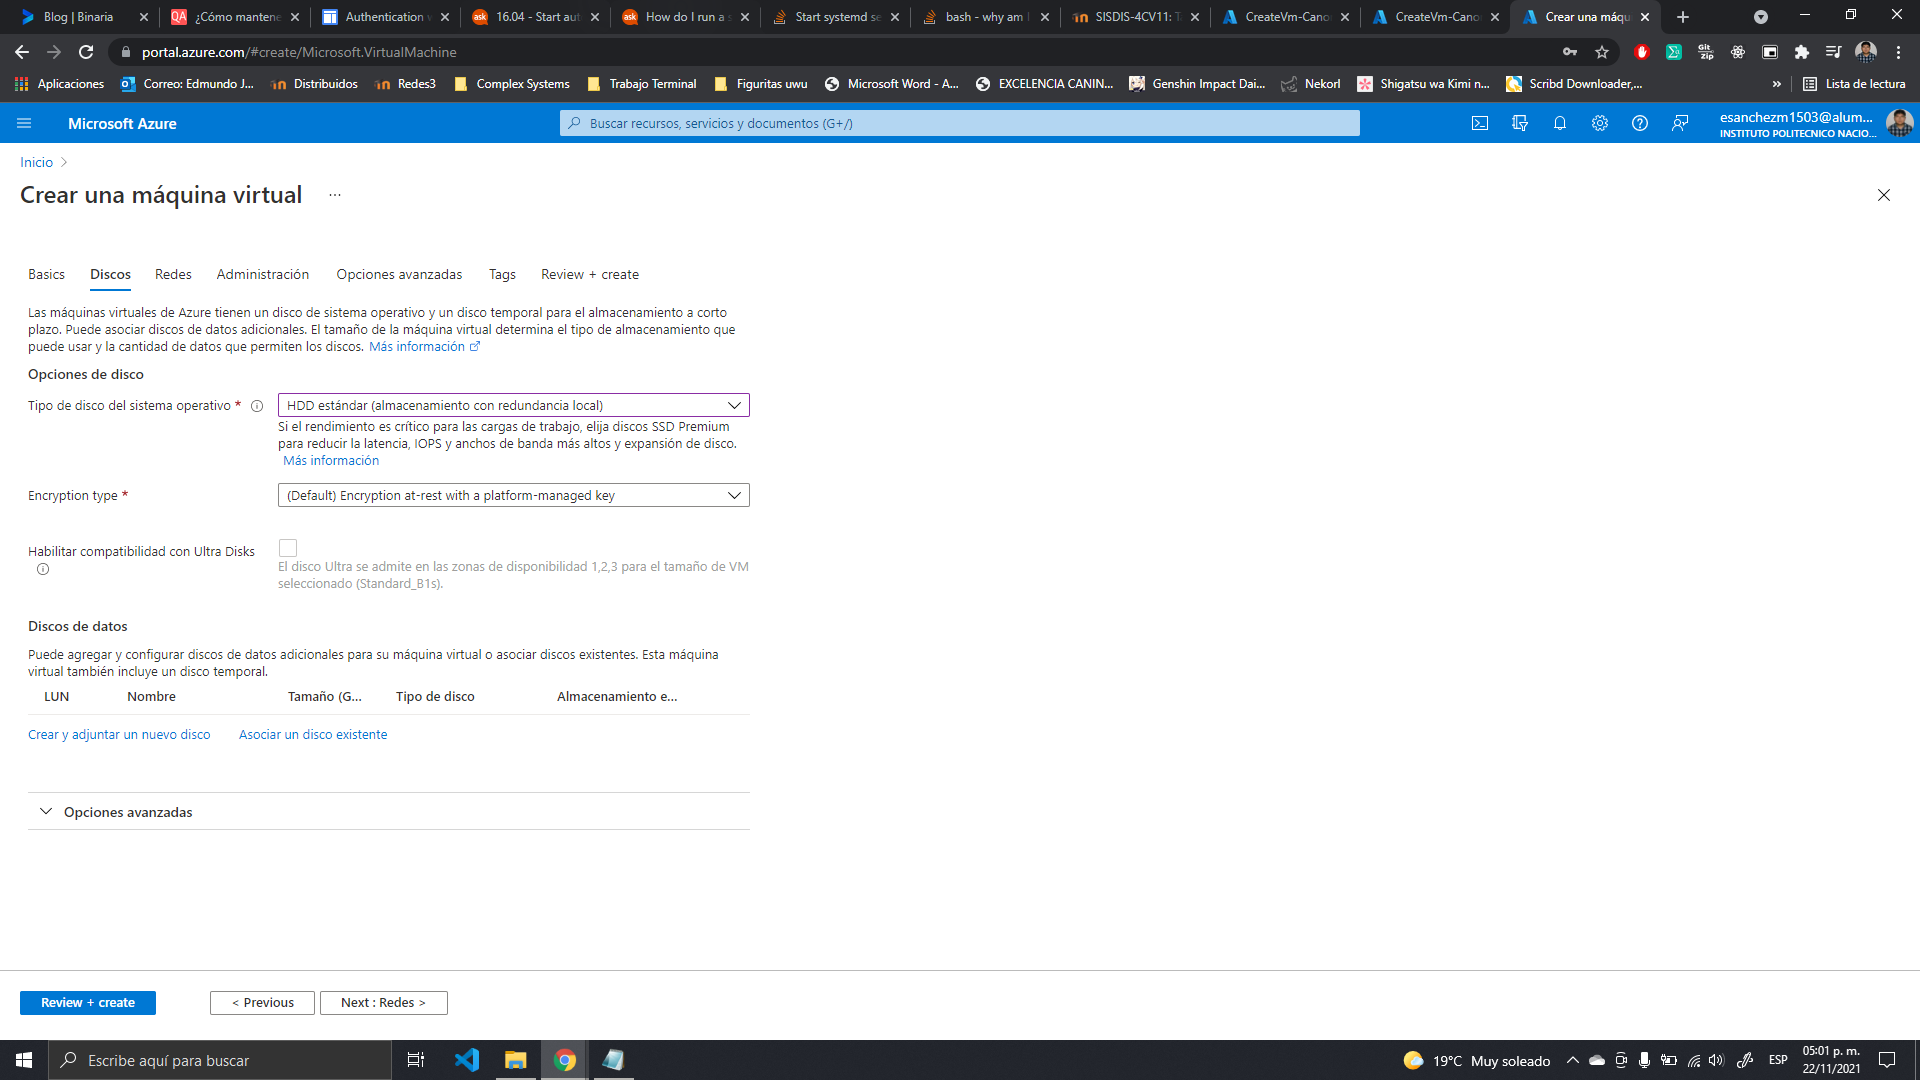
\includegraphics[scale=0.34]{resources/disco2.png}
			\caption{Configuración del tipo de disco de la maquina virtual.}\label{fig:picture}
		\end{figure}
		\begin{figure}[H]
			\centering
			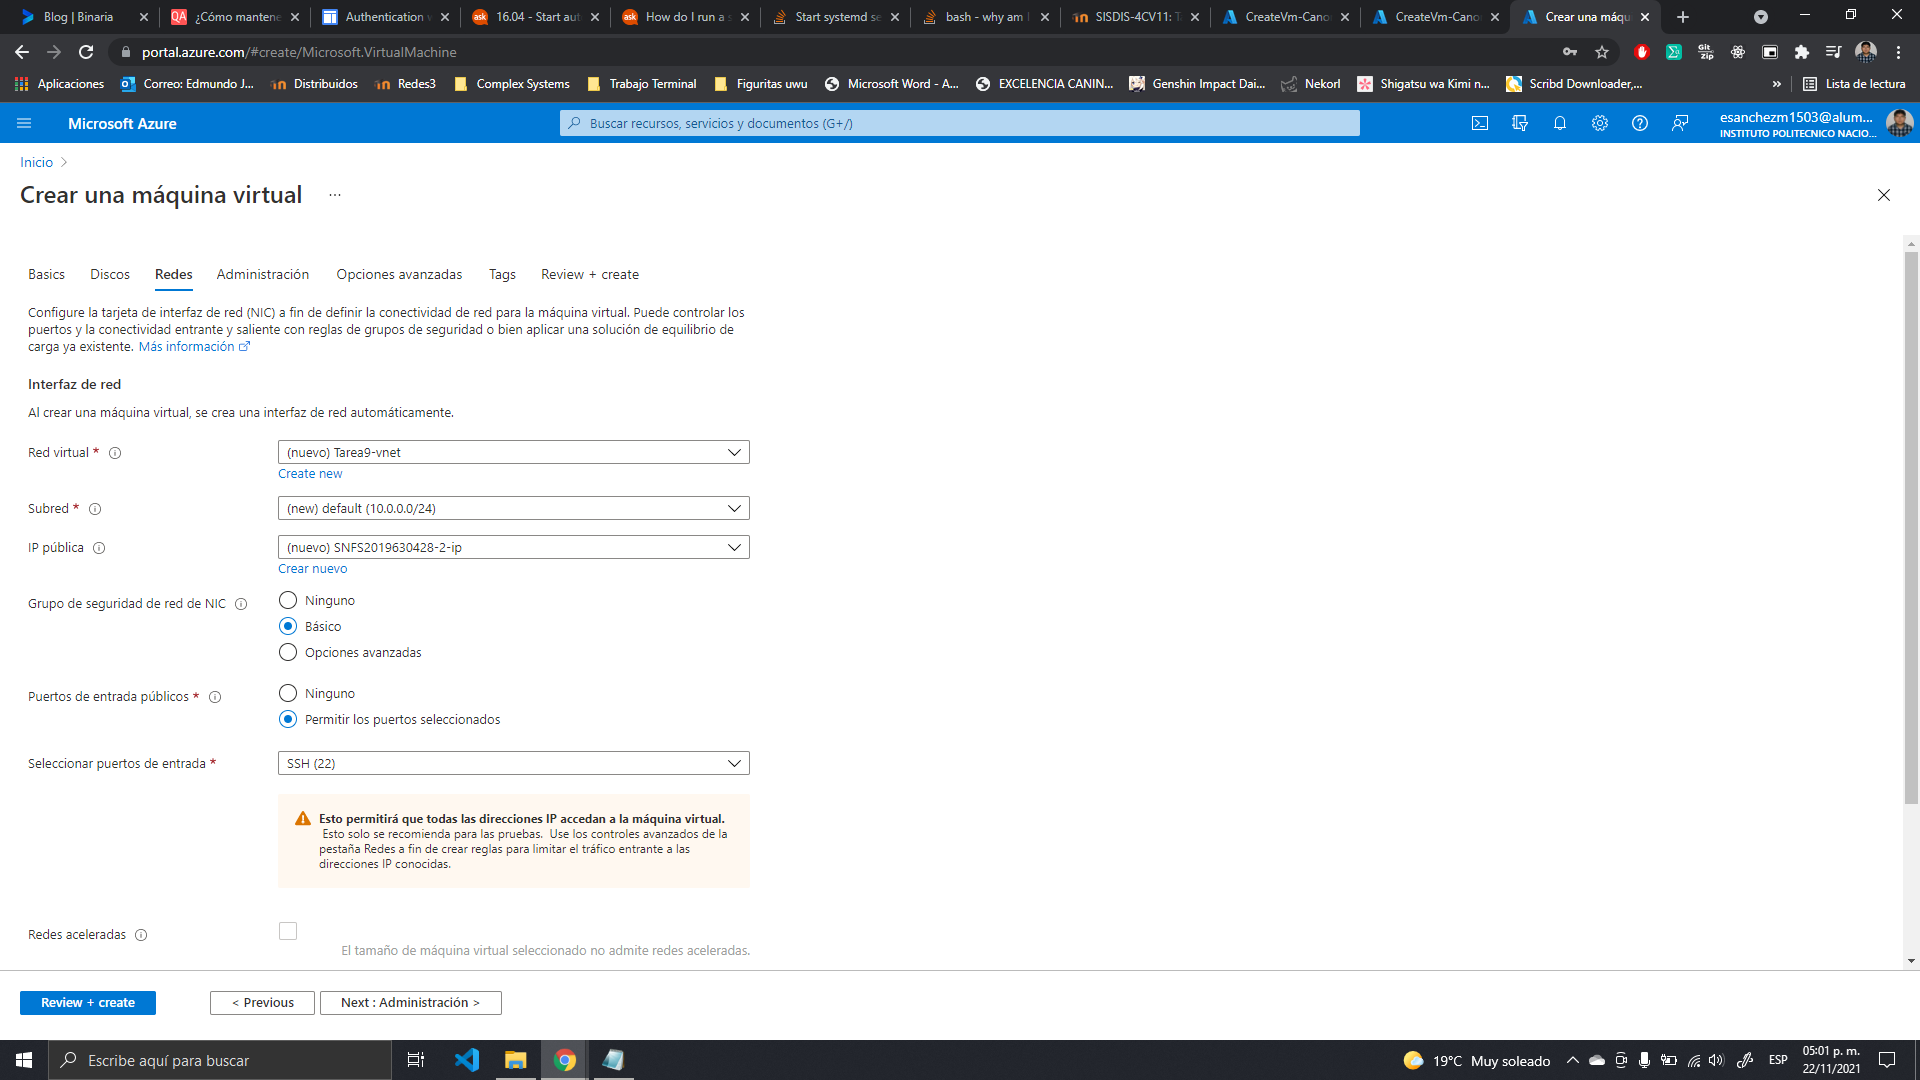
\includegraphics[scale=0.34]{resources/redes2.png}
			\caption{Información sobre la redes de la maquina virtual.}\label{fig:picture}
		\end{figure}
		\begin{figure}[H]
			\centering
			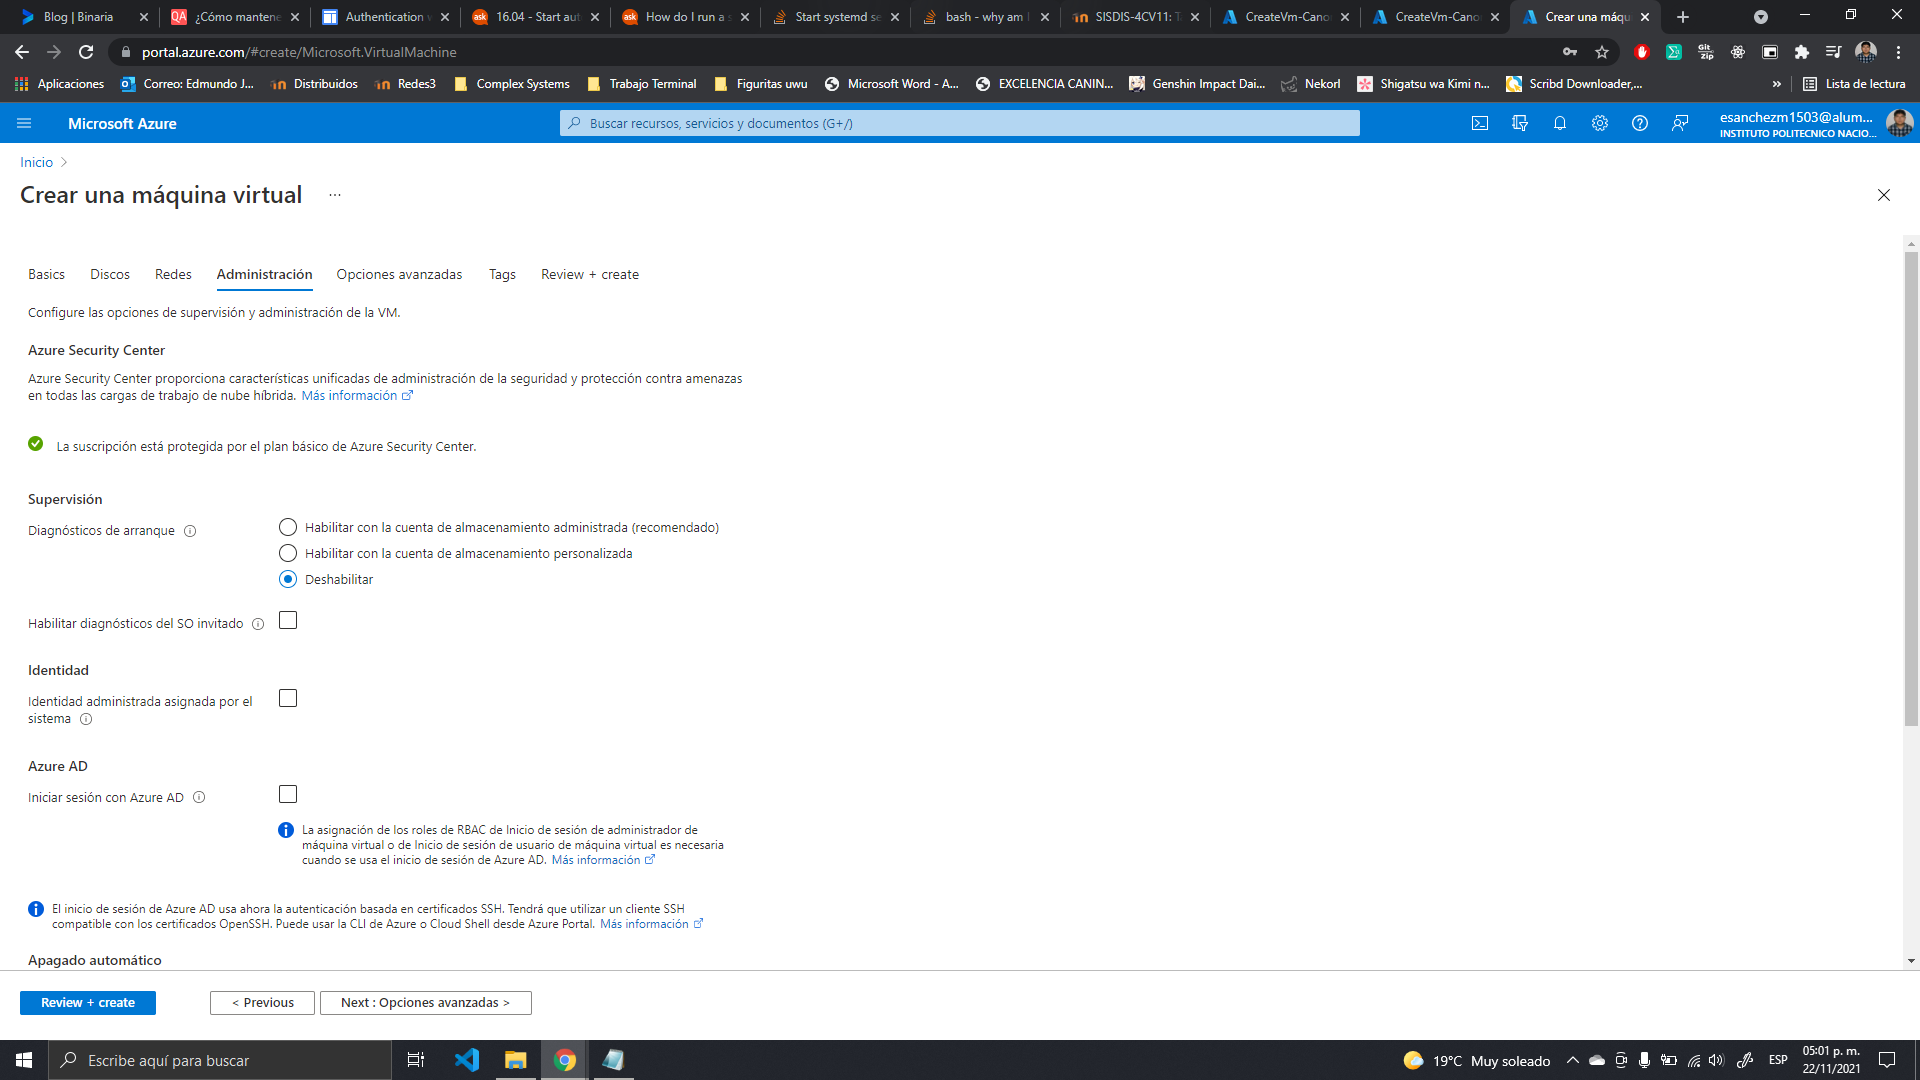
\includegraphics[scale=0.34]{resources/admin2.png}
			\caption{Configuración de la administración de la maquina virtual.}\label{fig:picture}
		\end{figure}
		\begin{figure}[H]
			\centering
			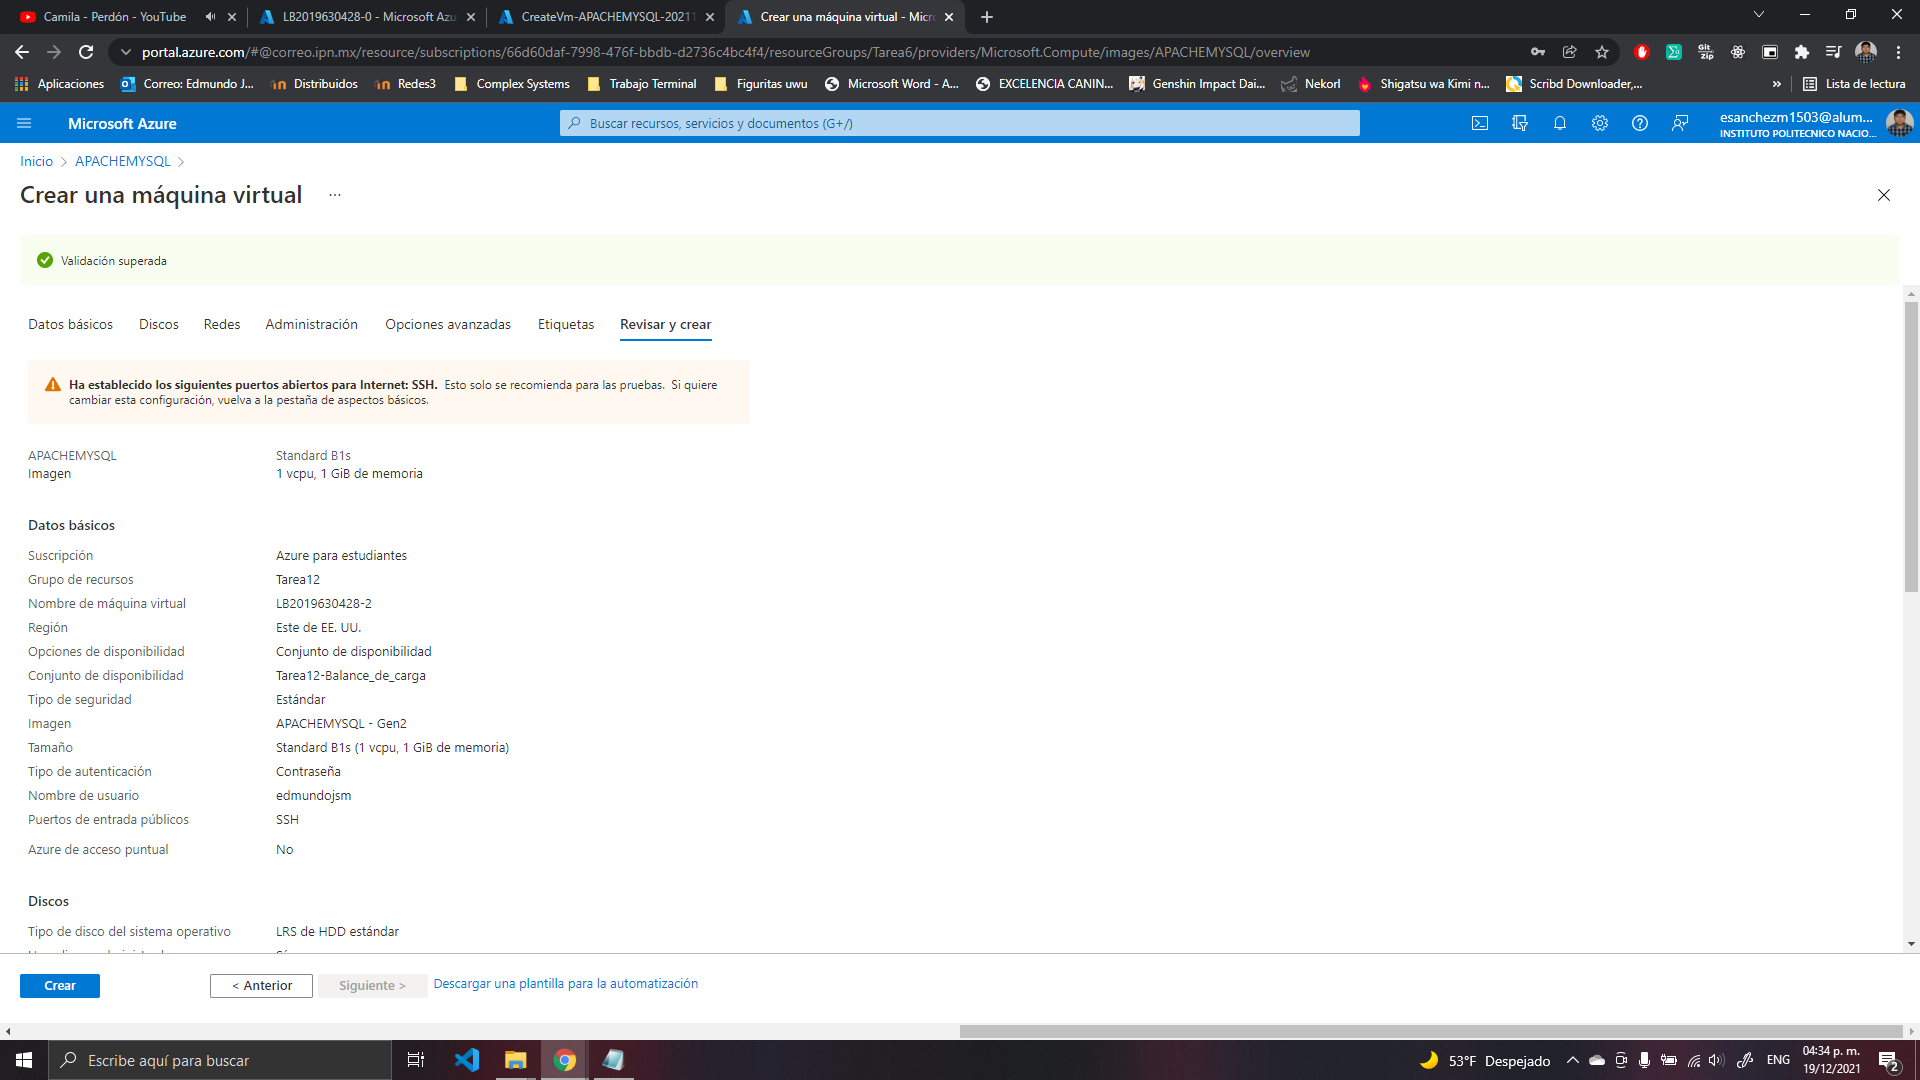
\includegraphics[scale=0.34]{resources/revisarycrear2.png}
			\caption{Creación de la maquina virtual.}\label{fig:picture}
		\end{figure}
		\begin{figure}[H]
			\centering
			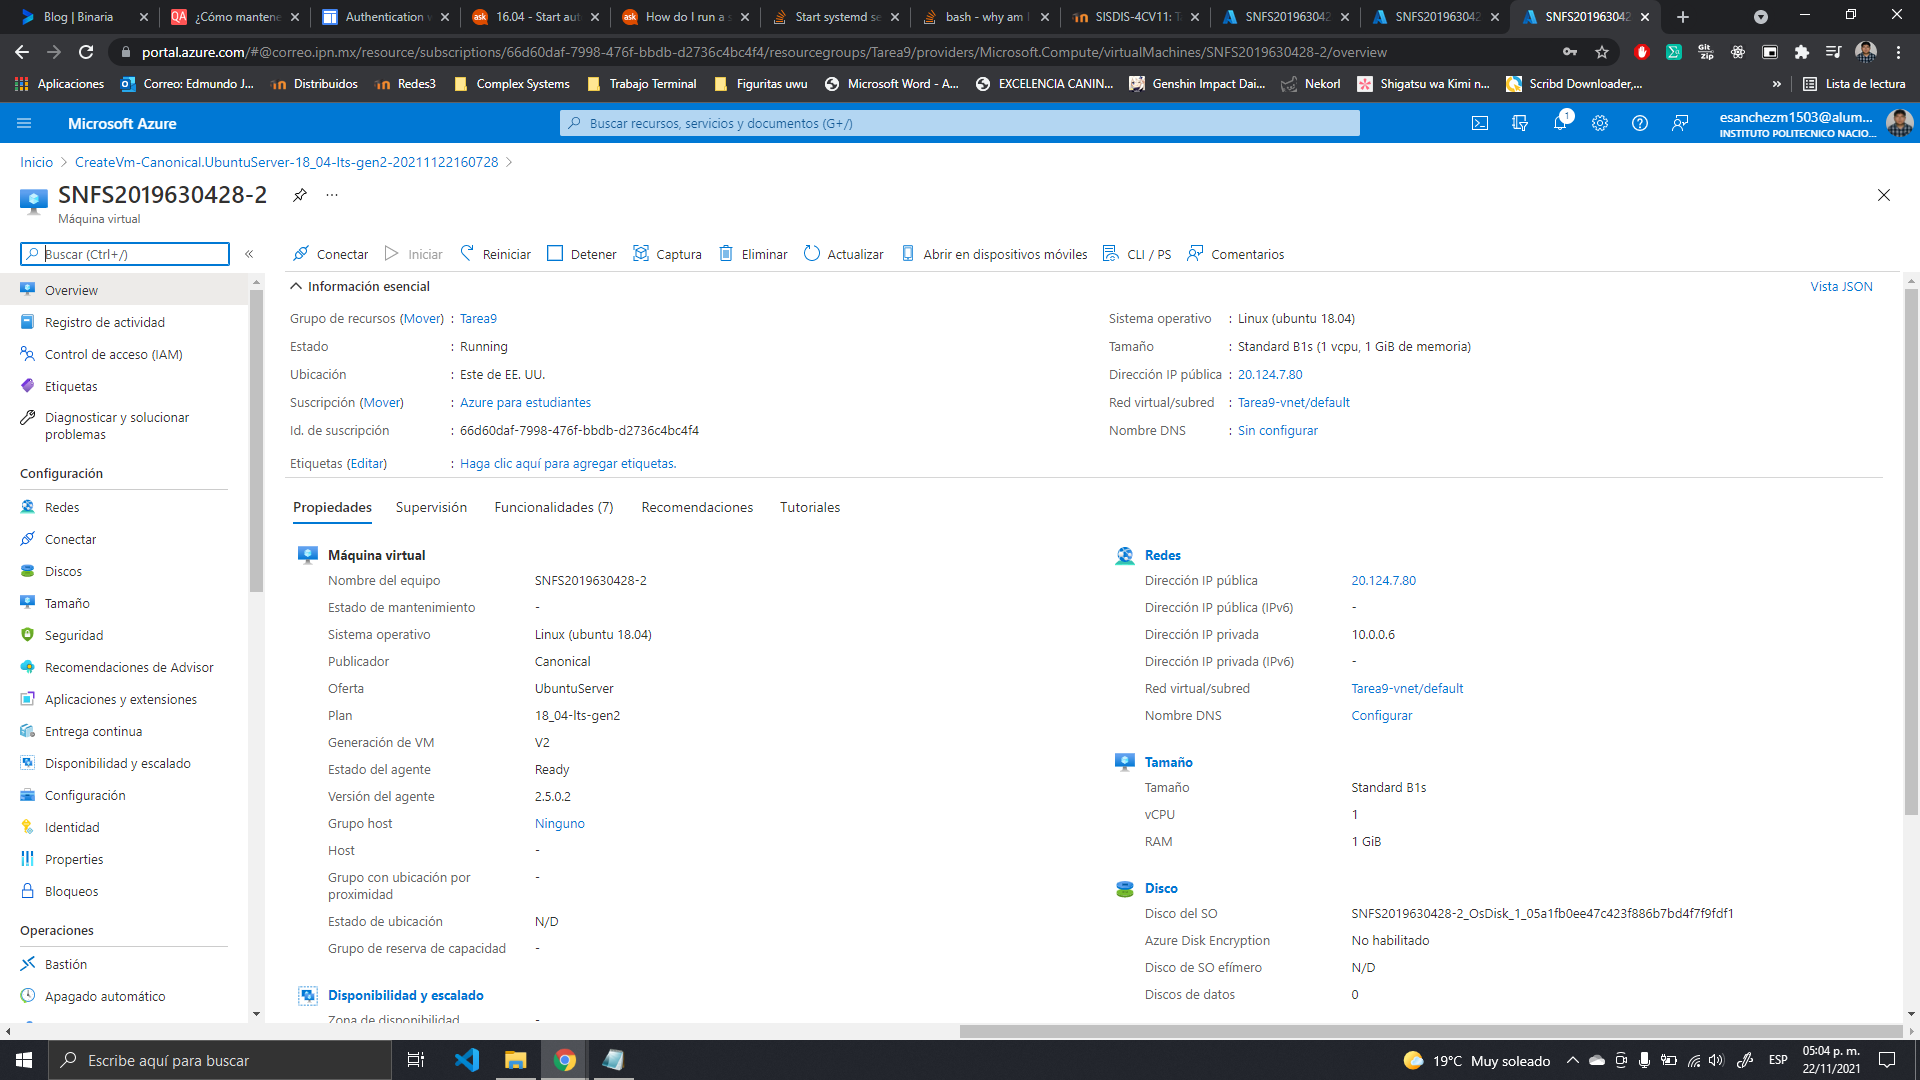
\includegraphics[scale=0.34]{resources/paneldecontrol2.png}
			\caption{Panel de control de la maquina virtual.}\label{fig:picture}
		\end{figure}		
		\subsection{Conexión SSH con el servidor, cliente 1 y cliente 2 de manera exitosa}
		En esta parte veremos la conexión del equipo de computo utilizado con las maquinas virtuales que serán nuestro servidor, cliente 1 y cliente 2.
		\begin{figure}[H]
			\centering
			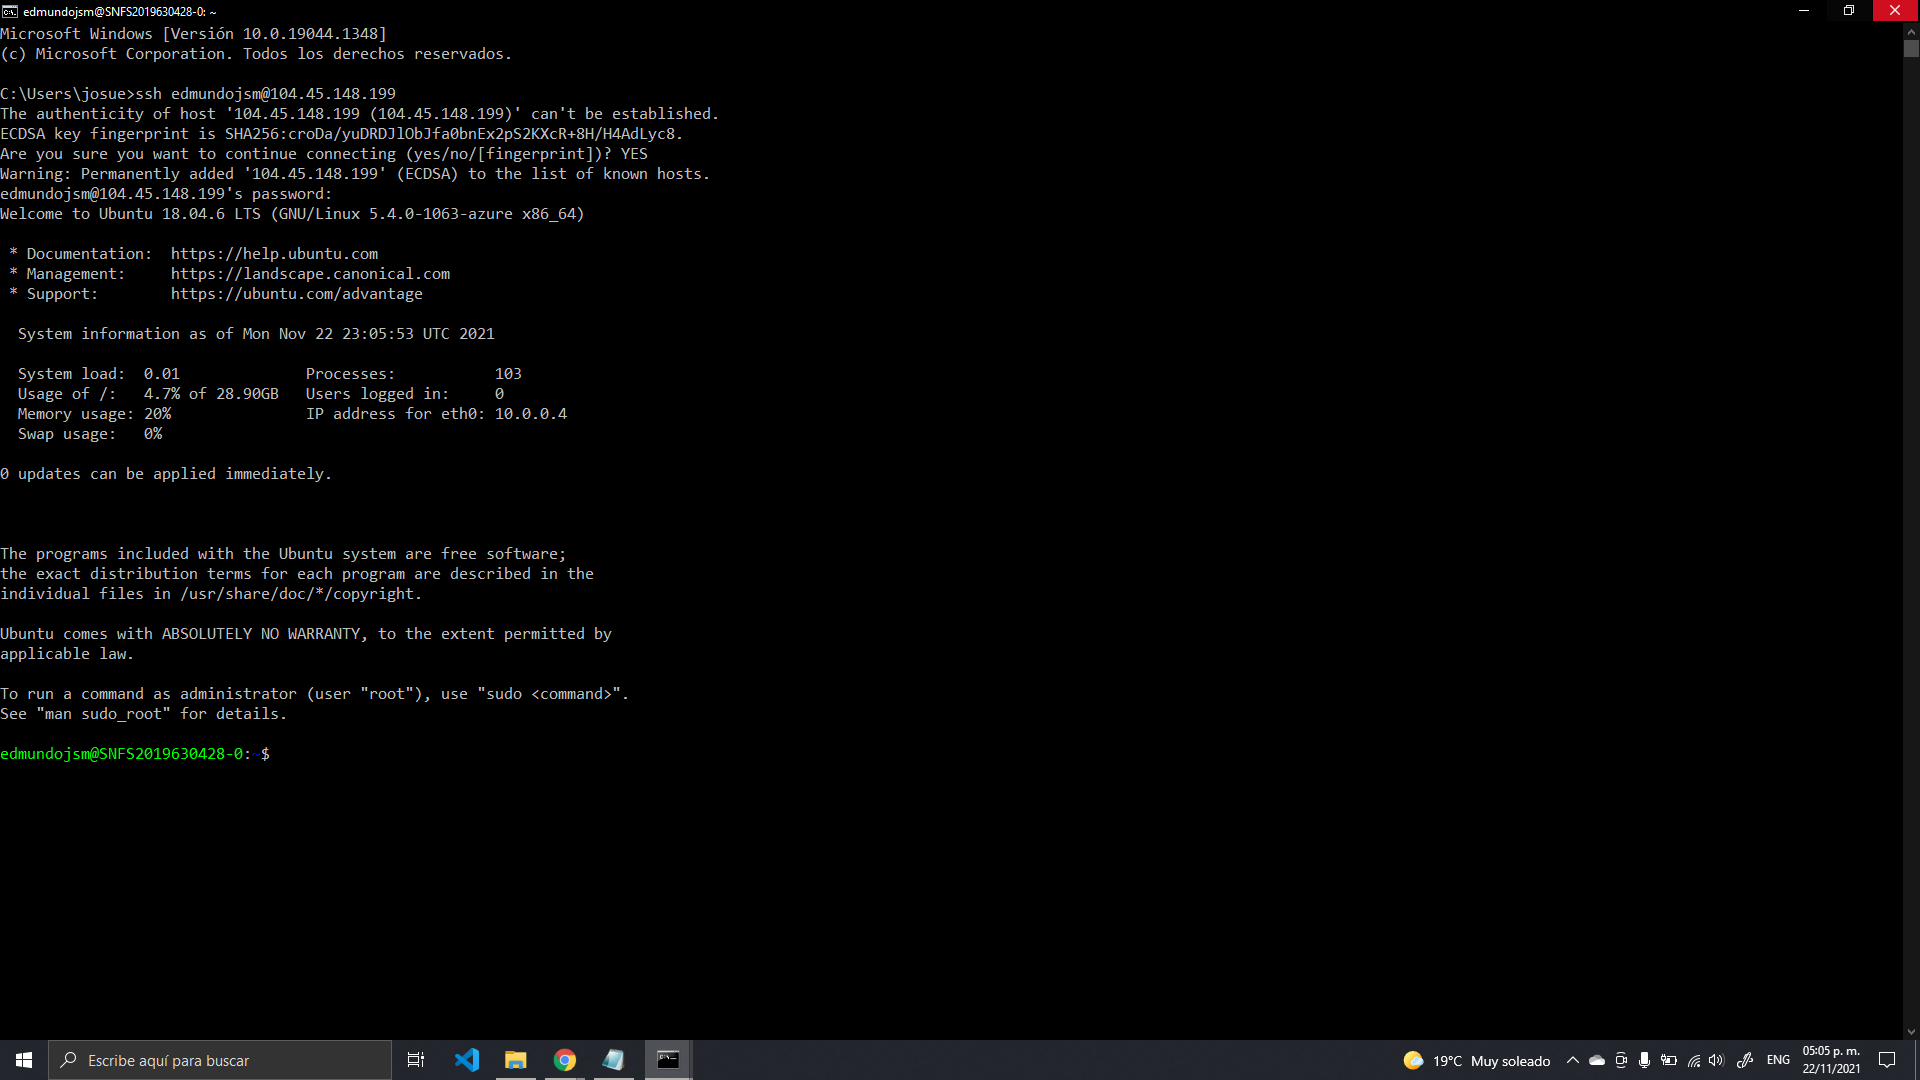
\includegraphics[scale=0.34]{resources/sshconexion0.png}
			\caption{Conexión con la maquina virtual que sera nuestro servidor.}\label{fig:picture}
		\end{figure}
		\begin{figure}[H]
			\centering
			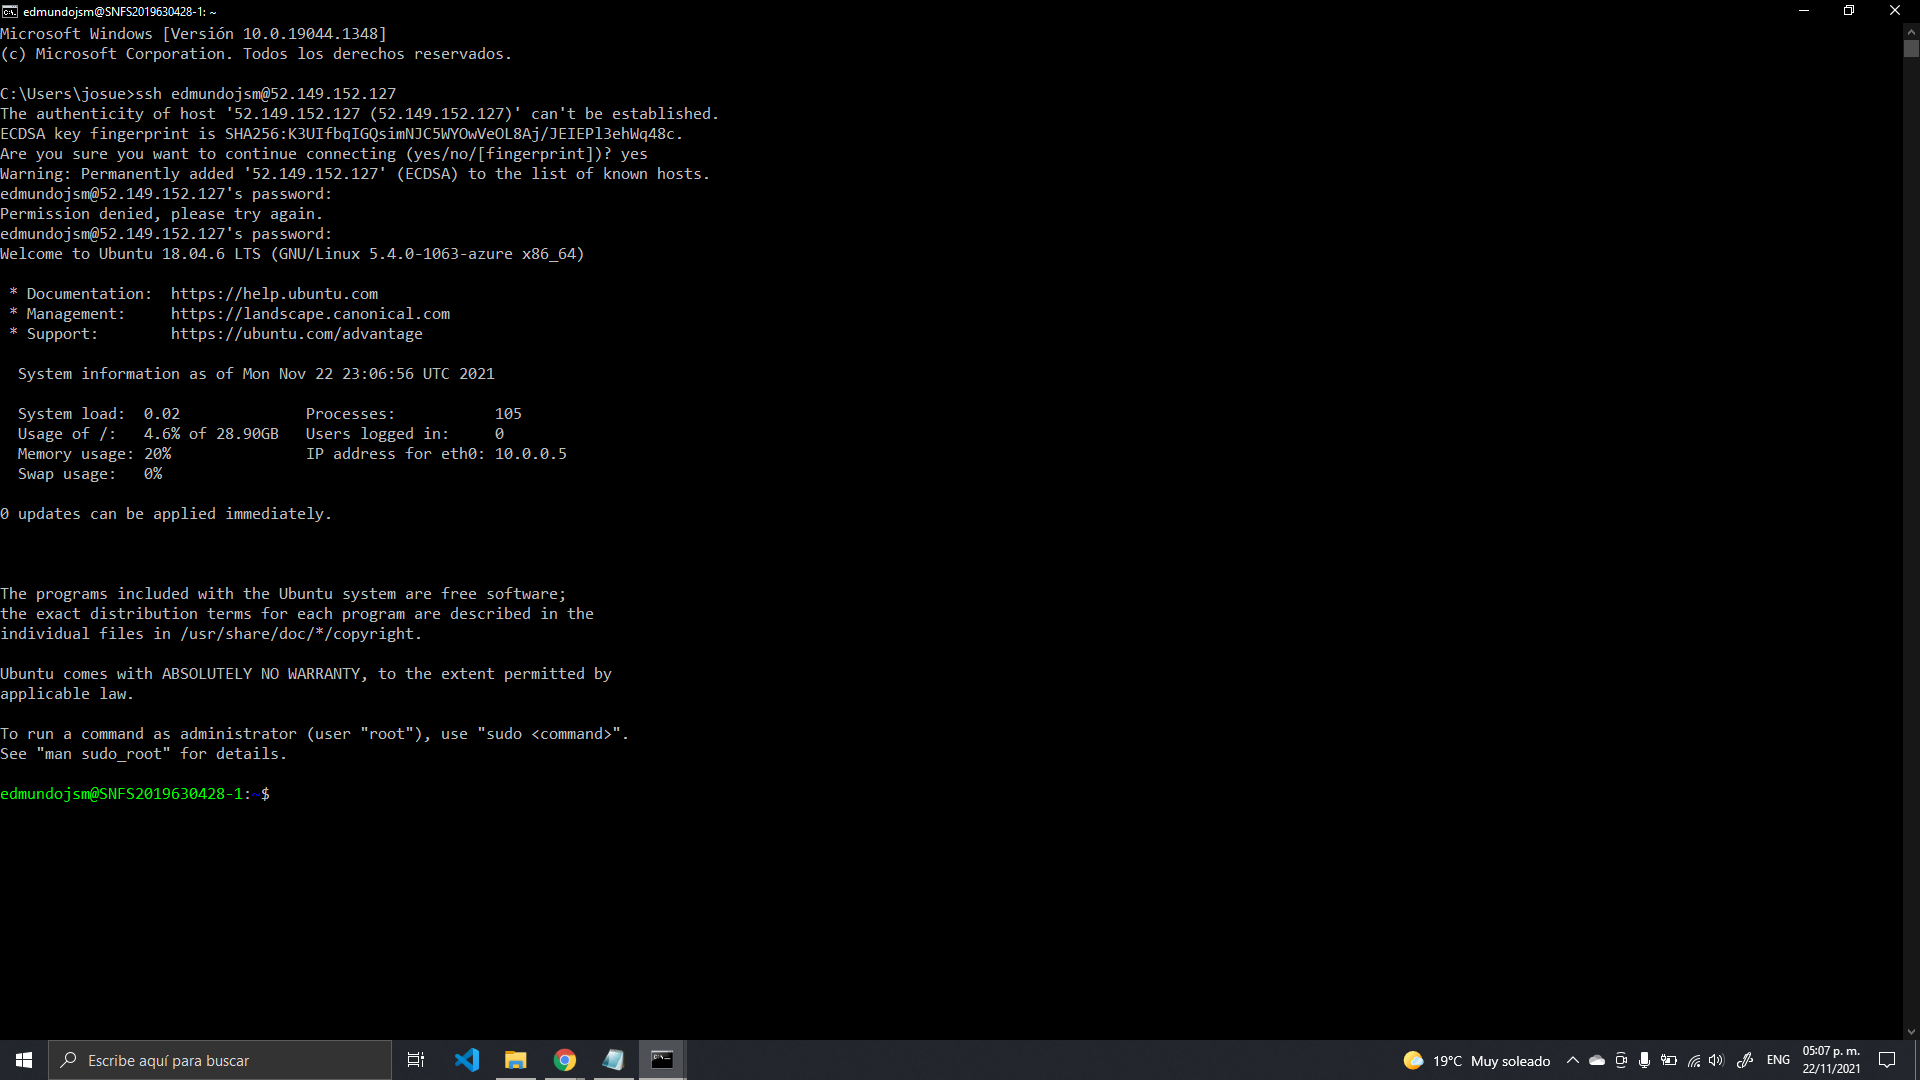
\includegraphics[scale=0.34]{resources/sshconexion1.png}
			\caption{Conexión con la maquina virtual que sera nuestro cliente 1.}\label{fig:picture}
		\end{figure}
		\begin{figure}[H]
			\centering
			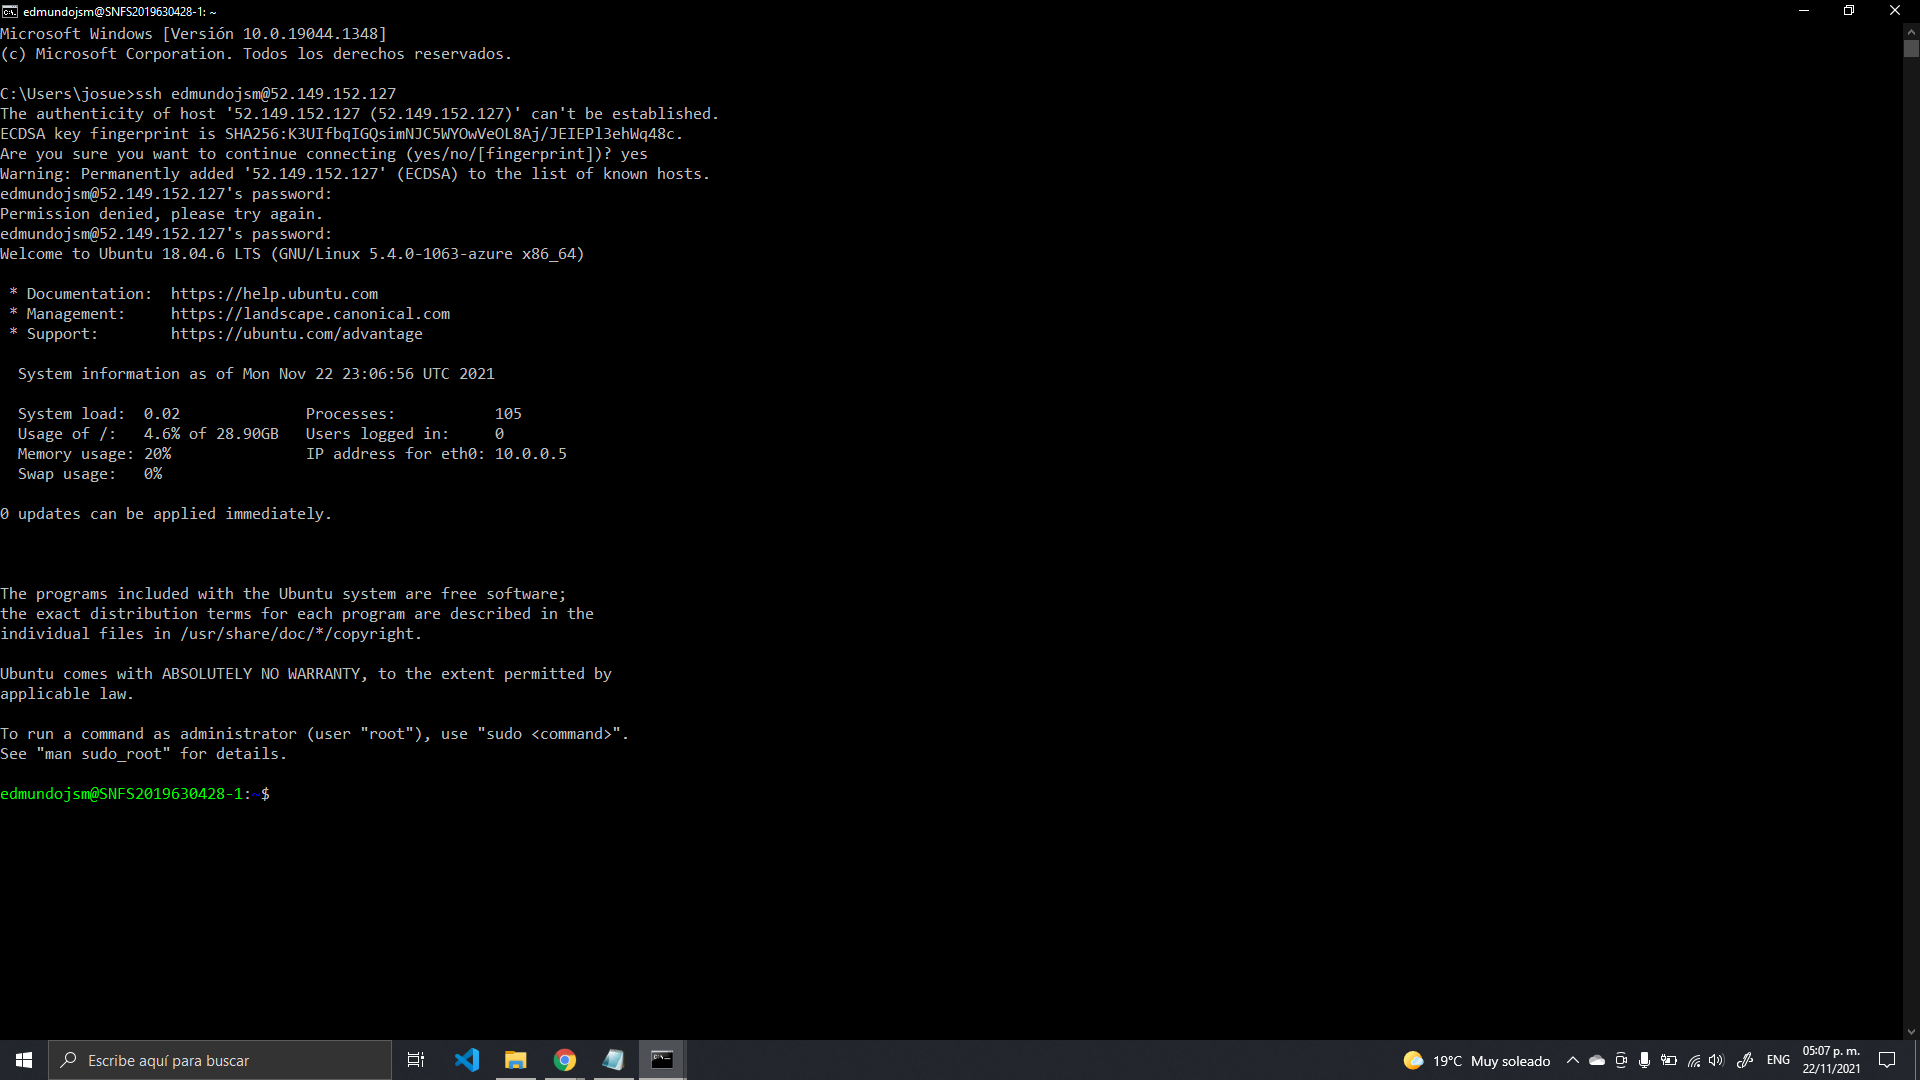
\includegraphics[scale=0.34]{resources/sshconexion1.png}
			\caption{Conexión con la maquina virtual que sera nuestro cliente 2.}\label{fig:picture}
		\end{figure}		
		\subsection{Instalación de paquetes a utilizar en el servidor}
		En esta parte veremos la instalación de los paquetes necesarios para la creación de un servidor NFS todo esto en la maquina virtual con terminación 0 que sera nuestro servidor.
		\begin{figure}[H]
			\centering
			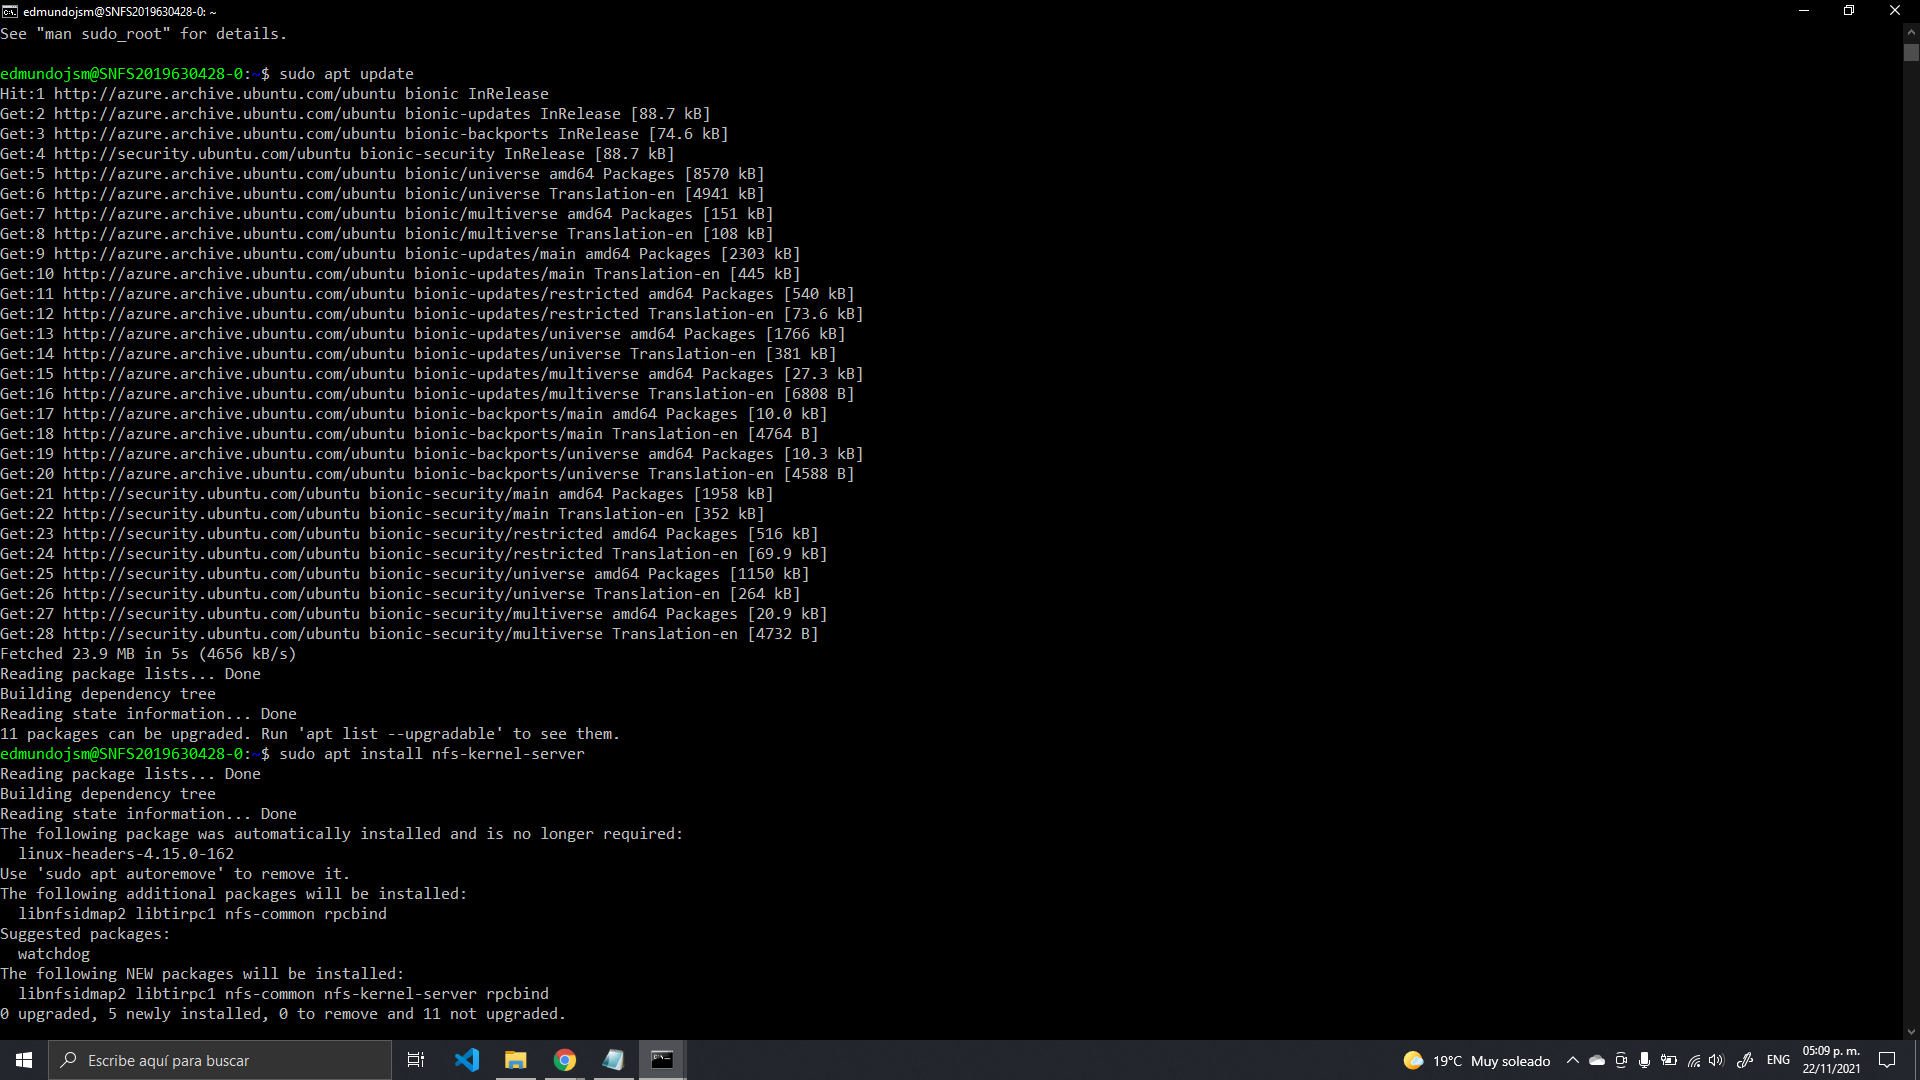
\includegraphics[scale=0.34]{resources/instalandoservidor1.png}
			\caption{Instalación de paquetes a utilizar en el servidor. Parte 1.}\label{fig:picture}
		\end{figure}
		\begin{figure}[H]
			\centering
			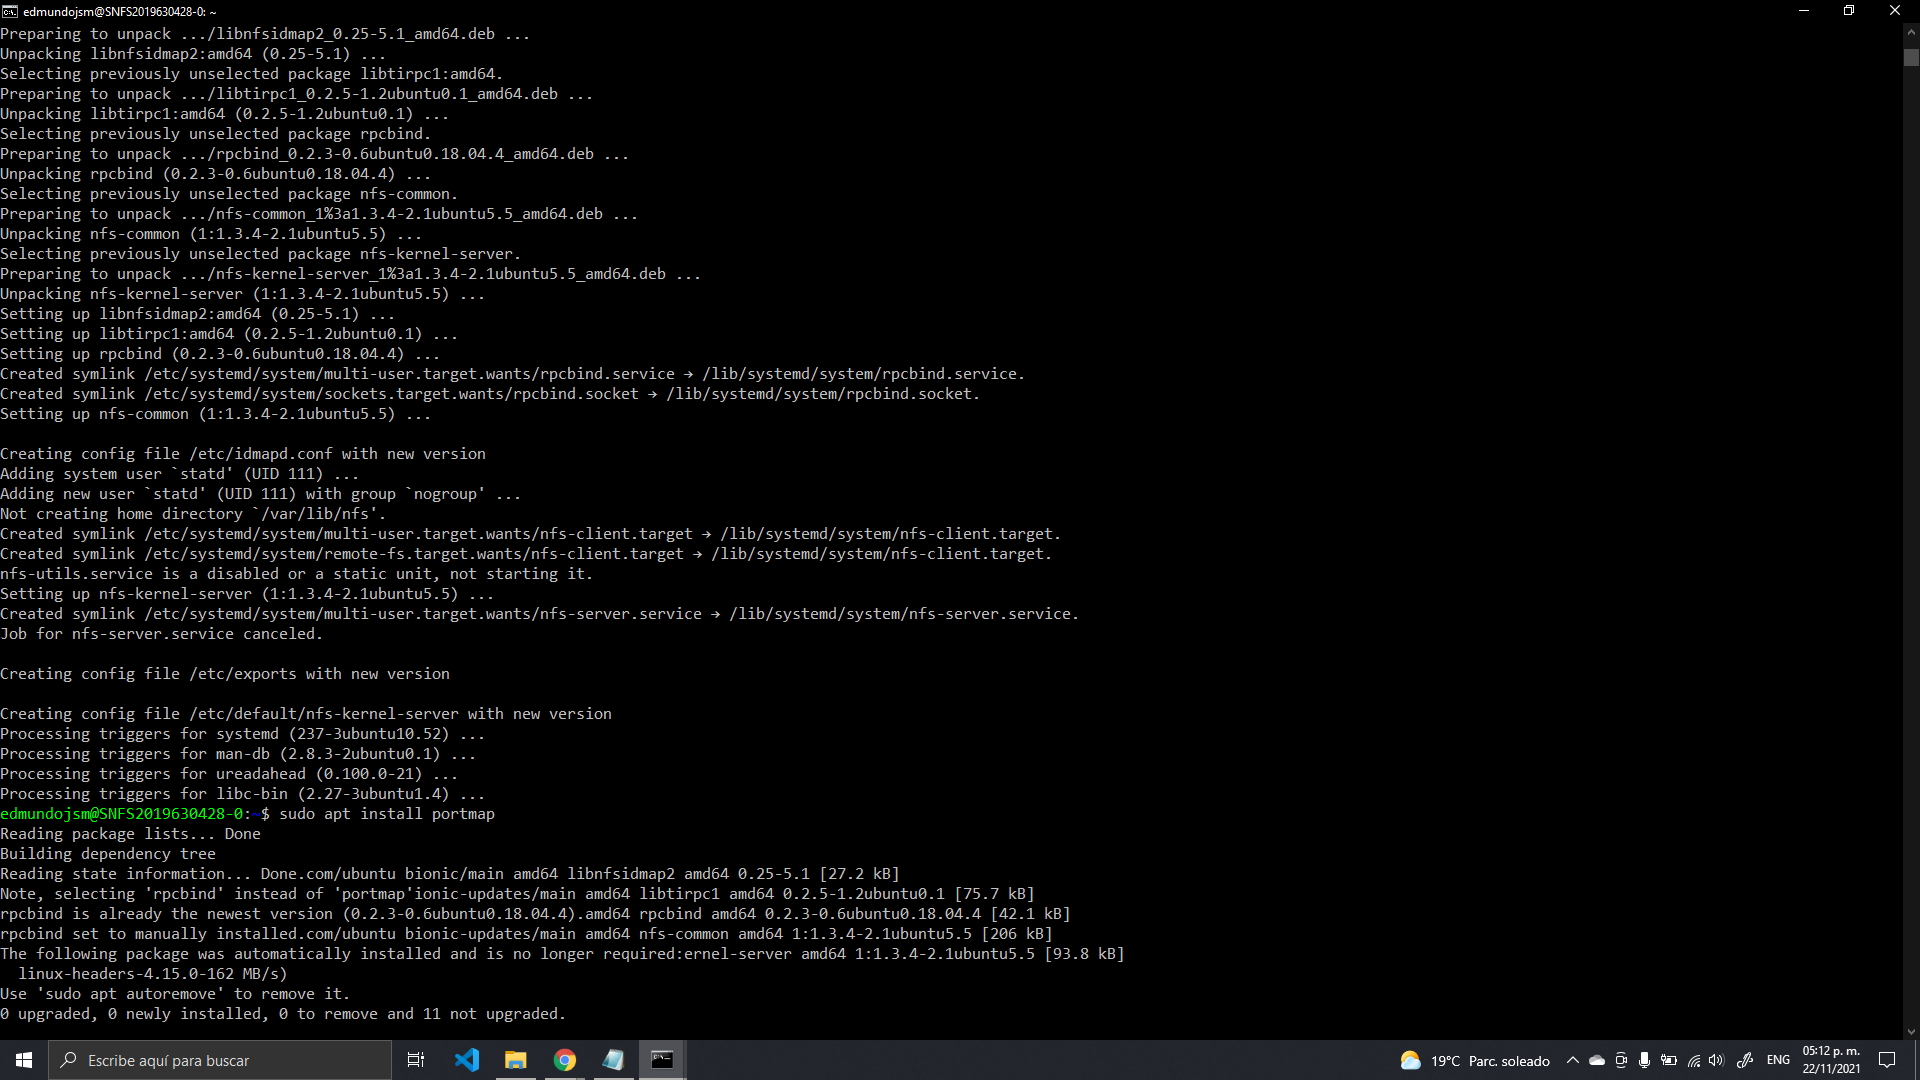
\includegraphics[scale=0.34]{resources/instalandoservidor2.png}
			\caption{Instalación de paquetes a utilizar en el servidor. Parte 2.}\label{fig:picture}
		\end{figure}
		\subsection{Instalación de paquetes a utilizar en el cliente 1}
		En esta parte veremos la instalación de los paquetes necesarios para la creación de un cliente NFS todo esto en la maquina virtual con terminación 1 que sera nuestro cliente 1.
		\begin{figure}[H]
			\centering
			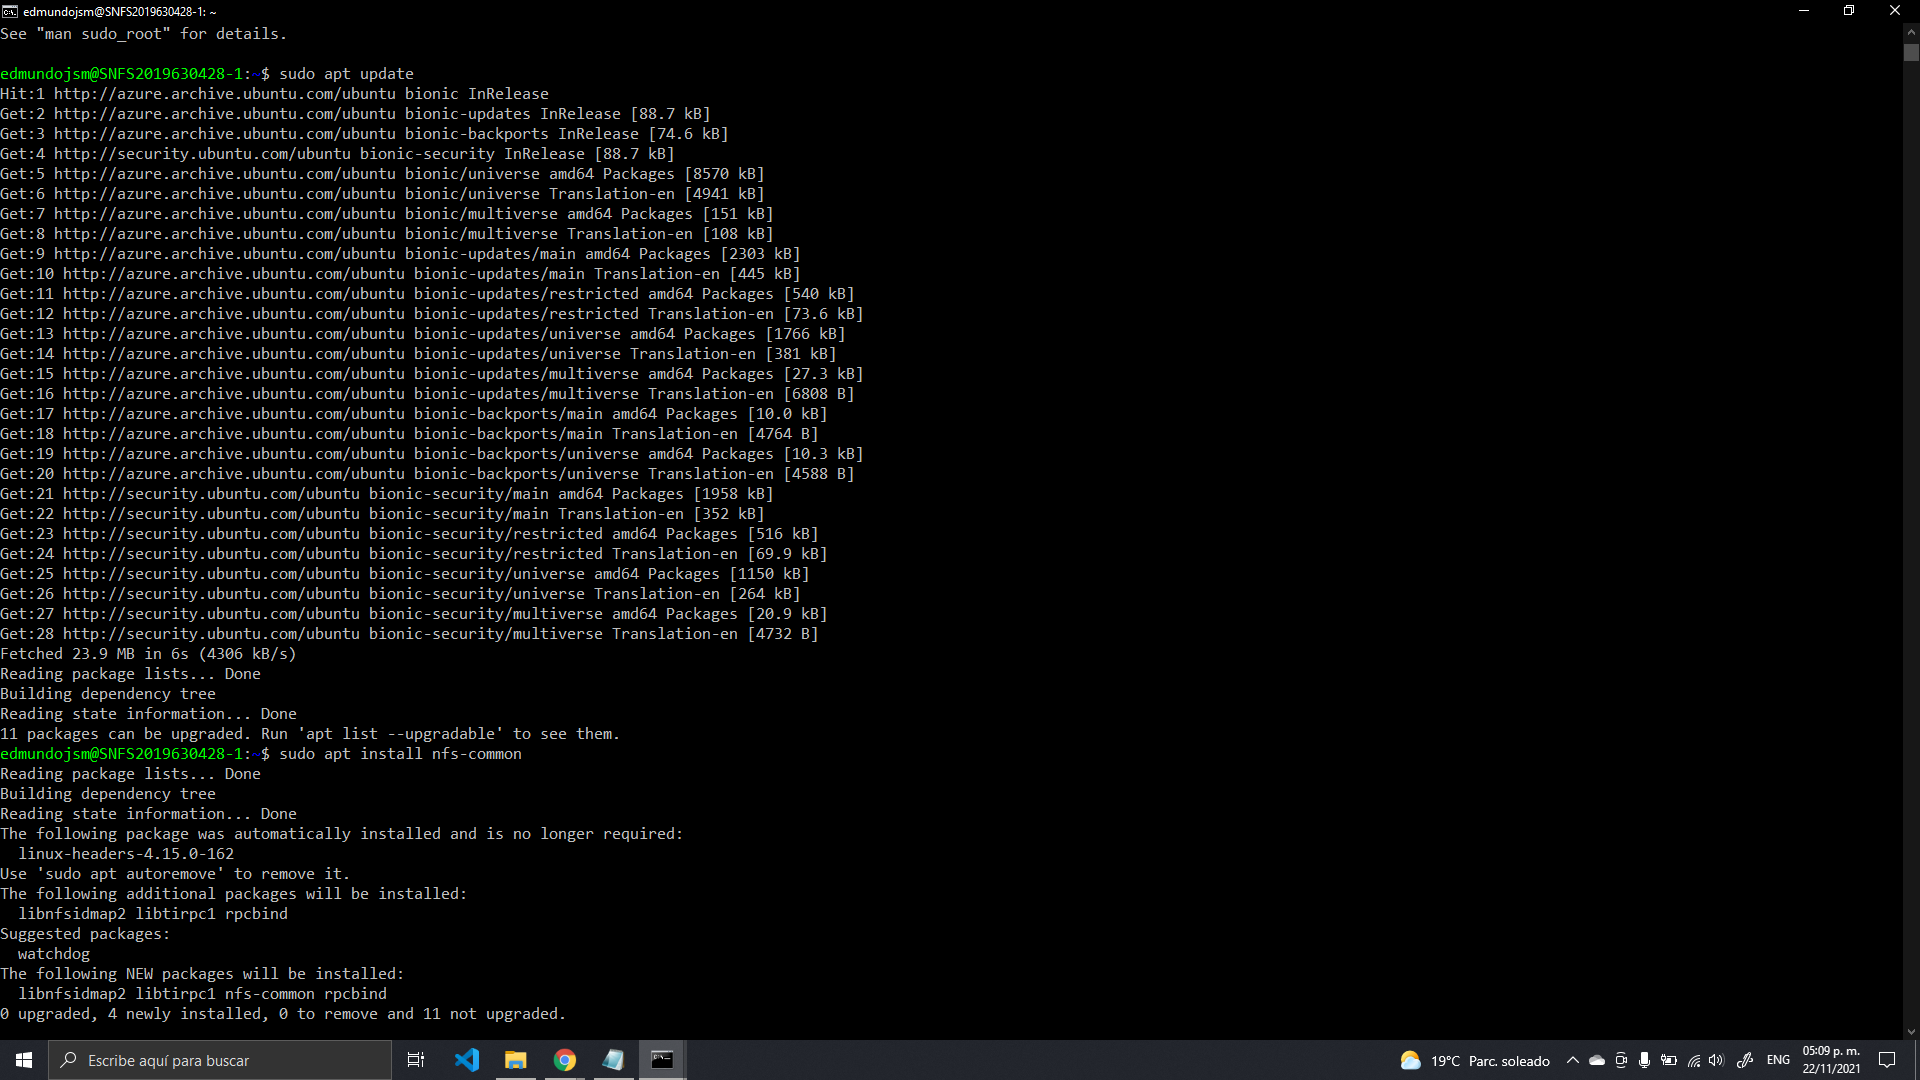
\includegraphics[scale=0.34]{resources/instalandocliente1.1.png}
			\caption{Instalación de paquetes a utilizar en el cliente 1. Parte 1.}\label{fig:picture}
		\end{figure}
		\begin{figure}[H]
			\centering
			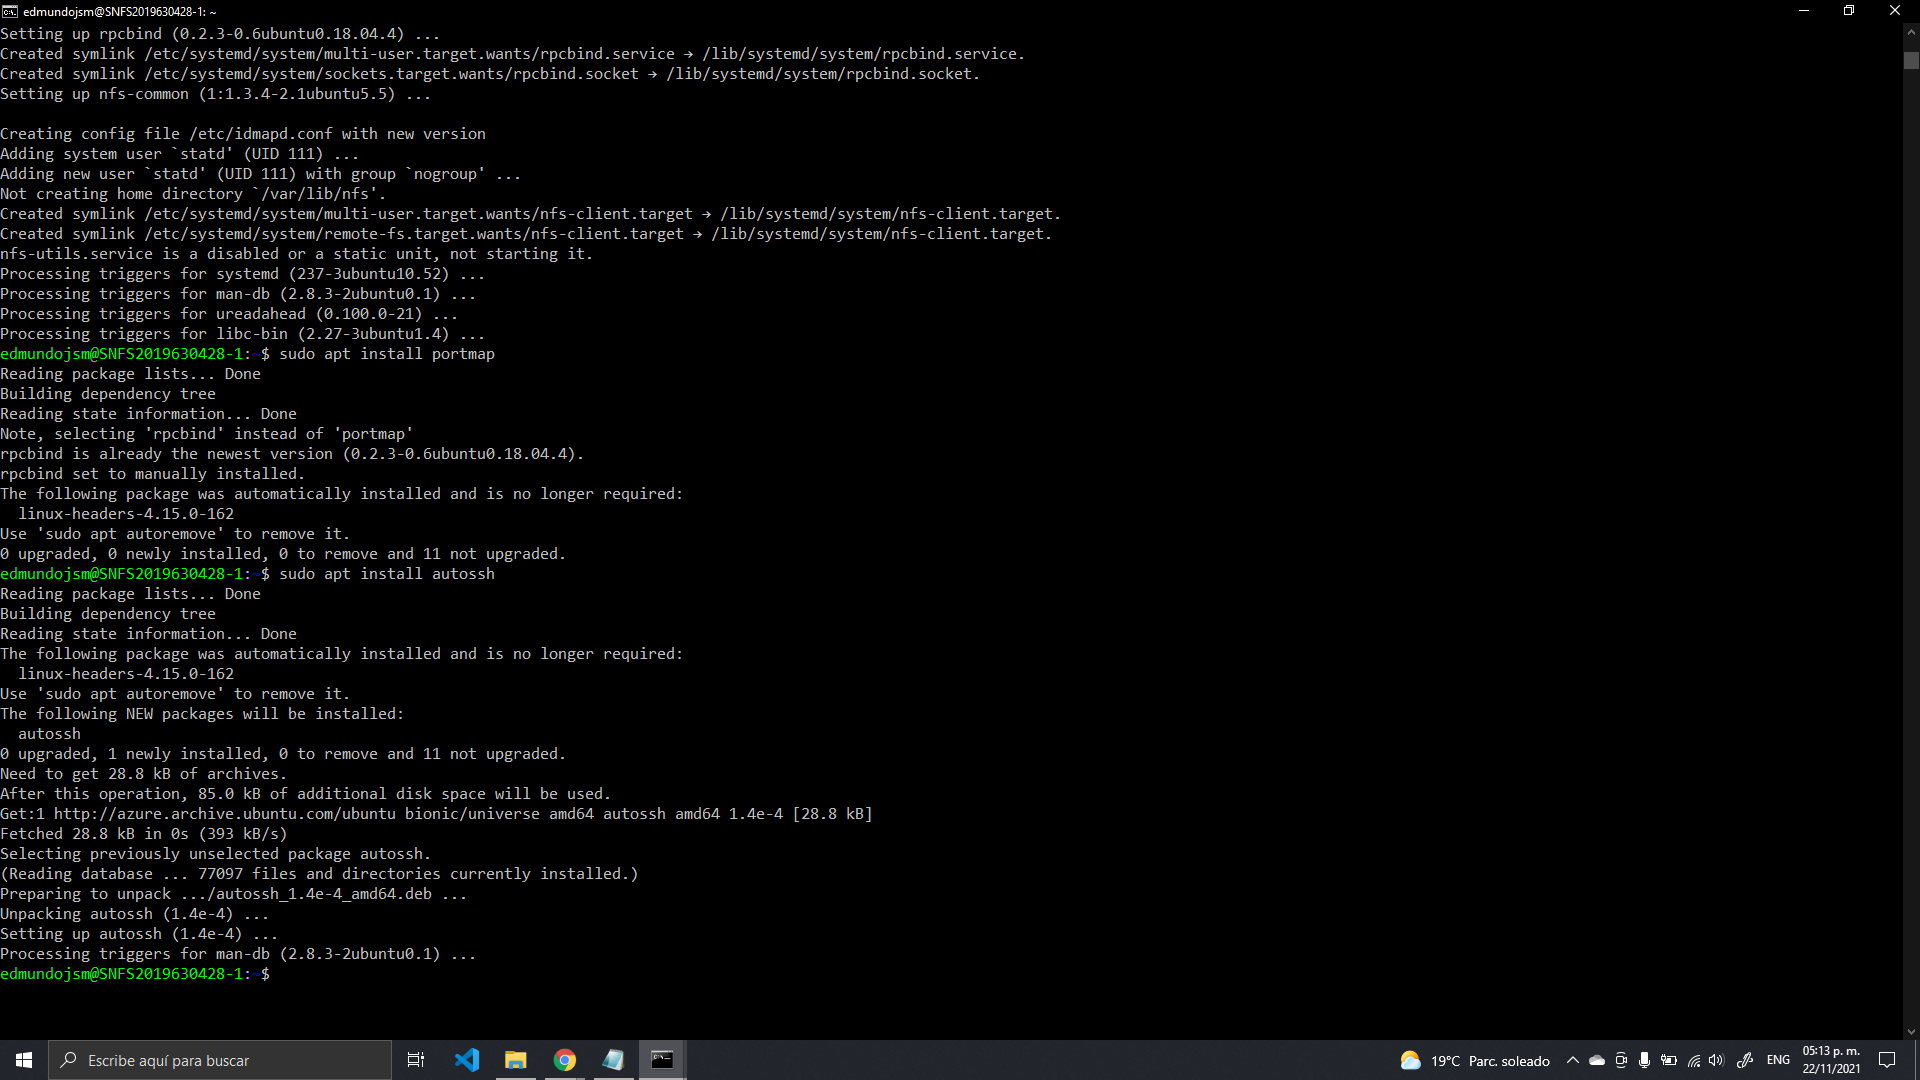
\includegraphics[scale=0.34]{resources/instalandocliente1.2.png}
			\caption{Instalación de paquetes a utilizar en el cliente 2. Parte 2.}\label{fig:picture}
		\end{figure}
		\subsection{Instalación de paquetes a utilizar en el cliente 2}
		En esta parte veremos la instalación de los paquetes necesarios para la creación de un cliente NFS todo esto en la maquina virtual con terminación 2 que sera nuestro cliente 2.
		\begin{figure}[H]
			\centering
			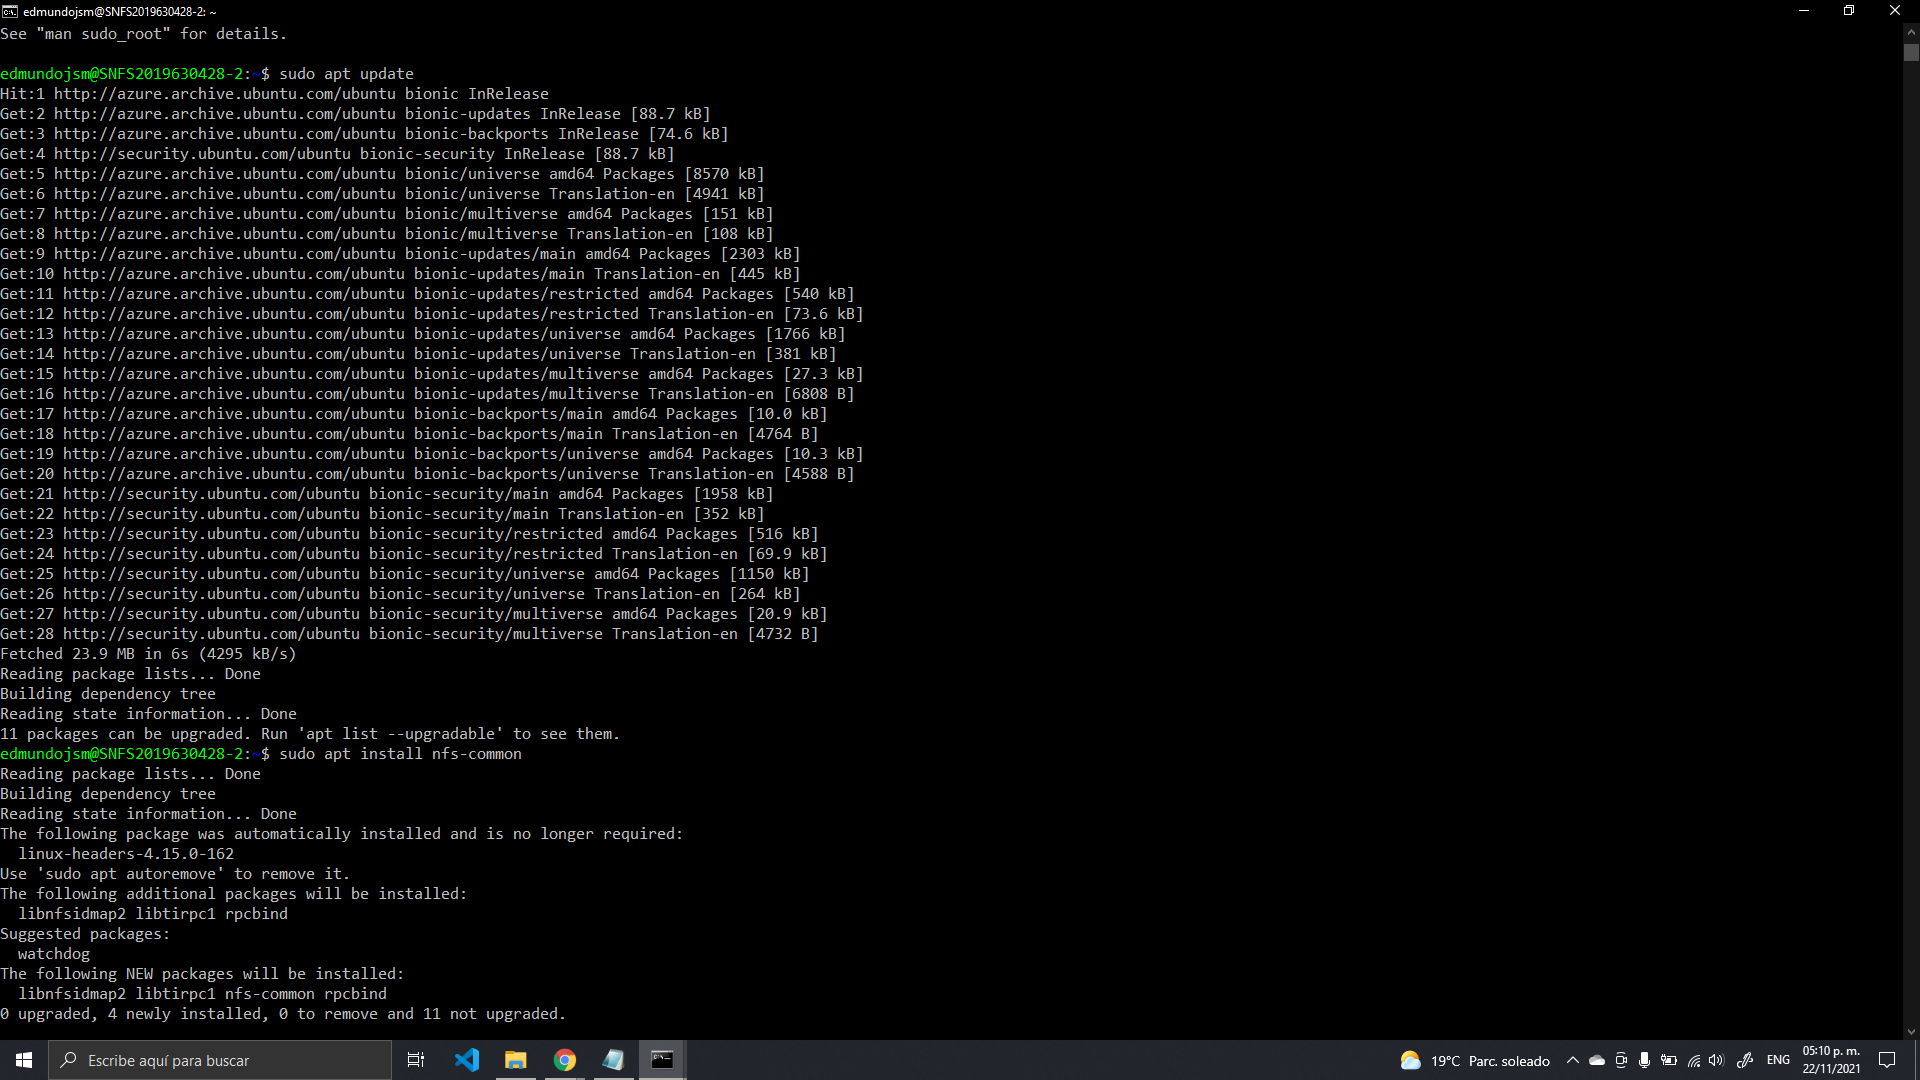
\includegraphics[scale=0.34]{resources/instalandocliente2.1.png}
			\caption{Instalación de paquetes a utilizar en el cliente 2. Parte 1.}\label{fig:picture}
		\end{figure}
		\begin{figure}[H]
			\centering
			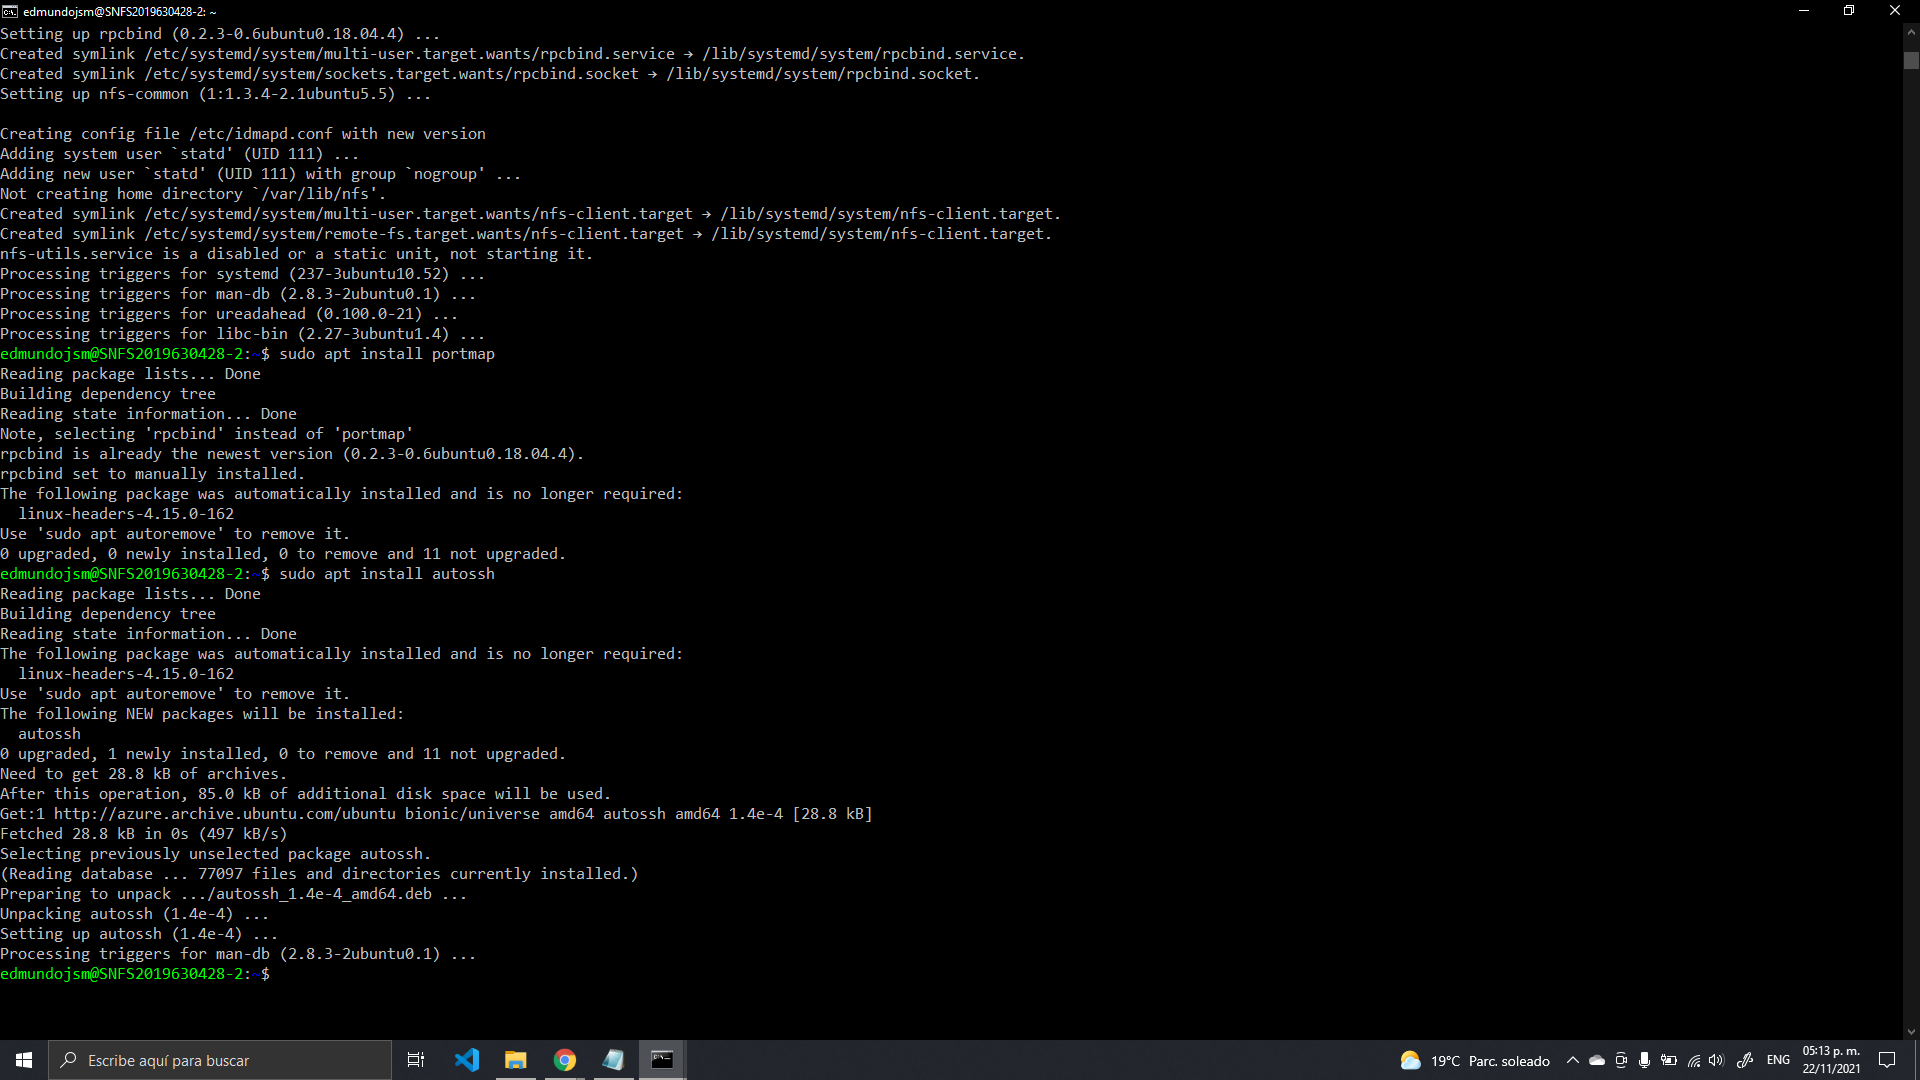
\includegraphics[scale=0.34]{resources/instalandocliente2.2.png}
			\caption{Instalación de paquetes a utilizar en el cliente 2. Parte 2.}\label{fig:picture}
		\end{figure}
		\subsection{Punto de montaje en el servidor}
		En esta parte veremos todo lo relacionado con la creación del punto de montaje en el servidor, es decir, la creación del directorio compartido, cambio  de propietario y permisos de este,  registro del directorio creado en la configuración de NFS, actualización de la tabla de file systems exportados por NFS y reinicio del servicio NFS.
		\begin{figure}[H]
			\centering
			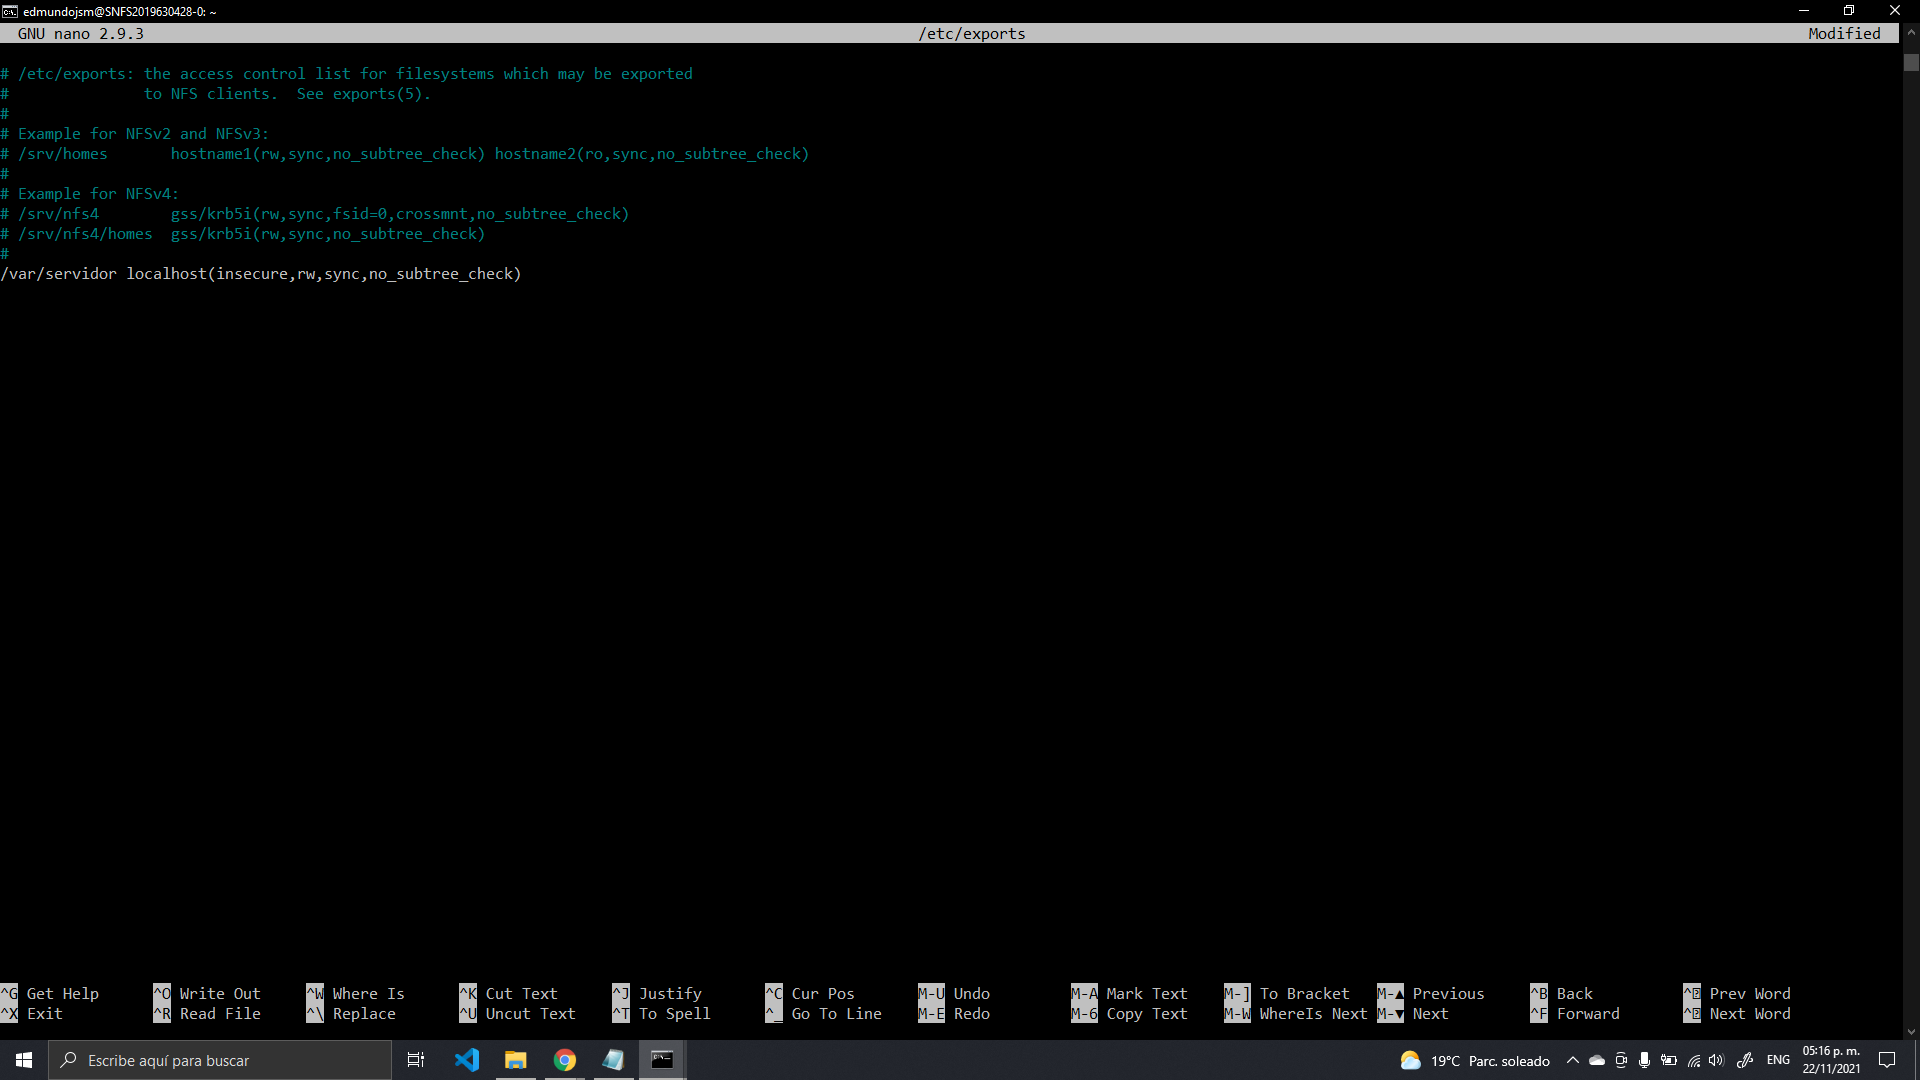
\includegraphics[scale=0.34]{resources/servidor1.png}
			\caption{Punto de montaje en el servidor. Parte 1.}\label{fig:picture}
		\end{figure}
		\begin{figure}[H]
			\centering
			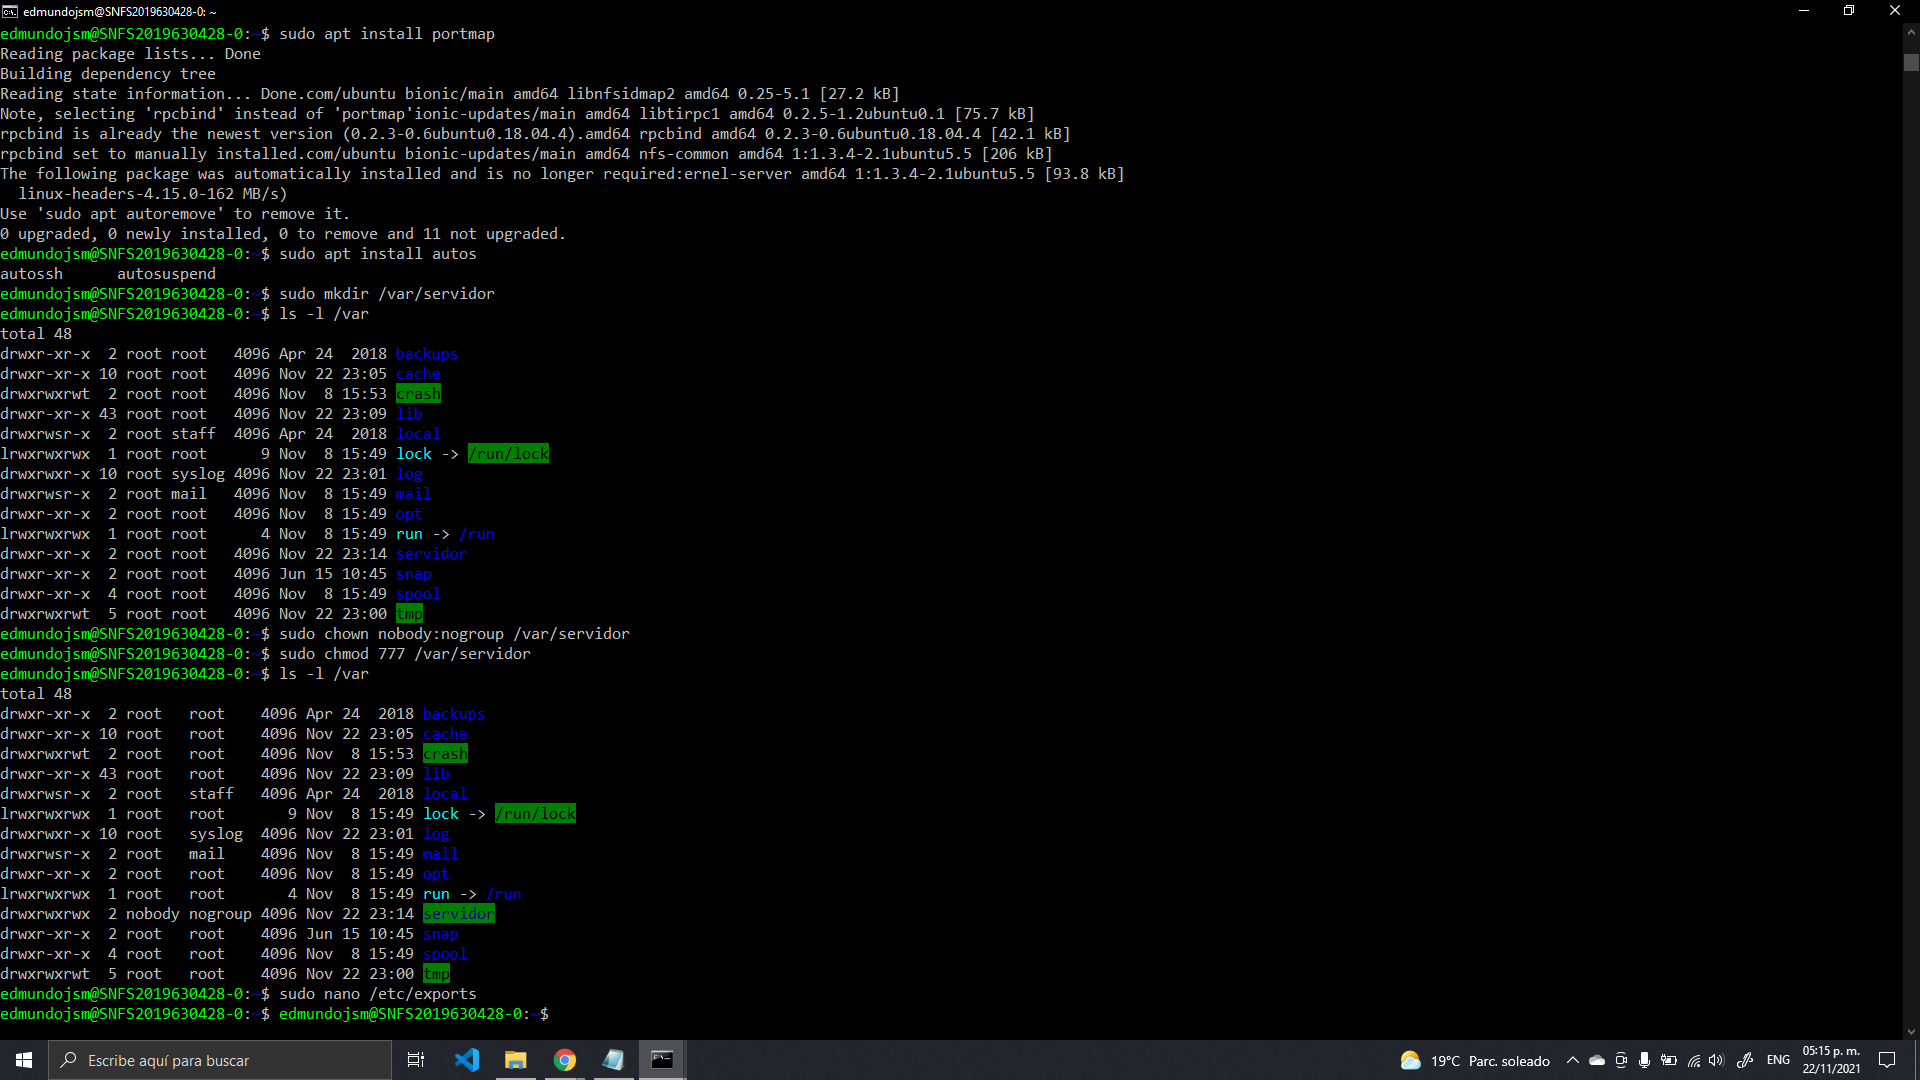
\includegraphics[scale=0.34]{resources/servidor2.png}
			\caption{Punto de montaje en el servidor. Parte 2.}\label{fig:picture}
		\end{figure}
		\begin{figure}[H]
			\centering
			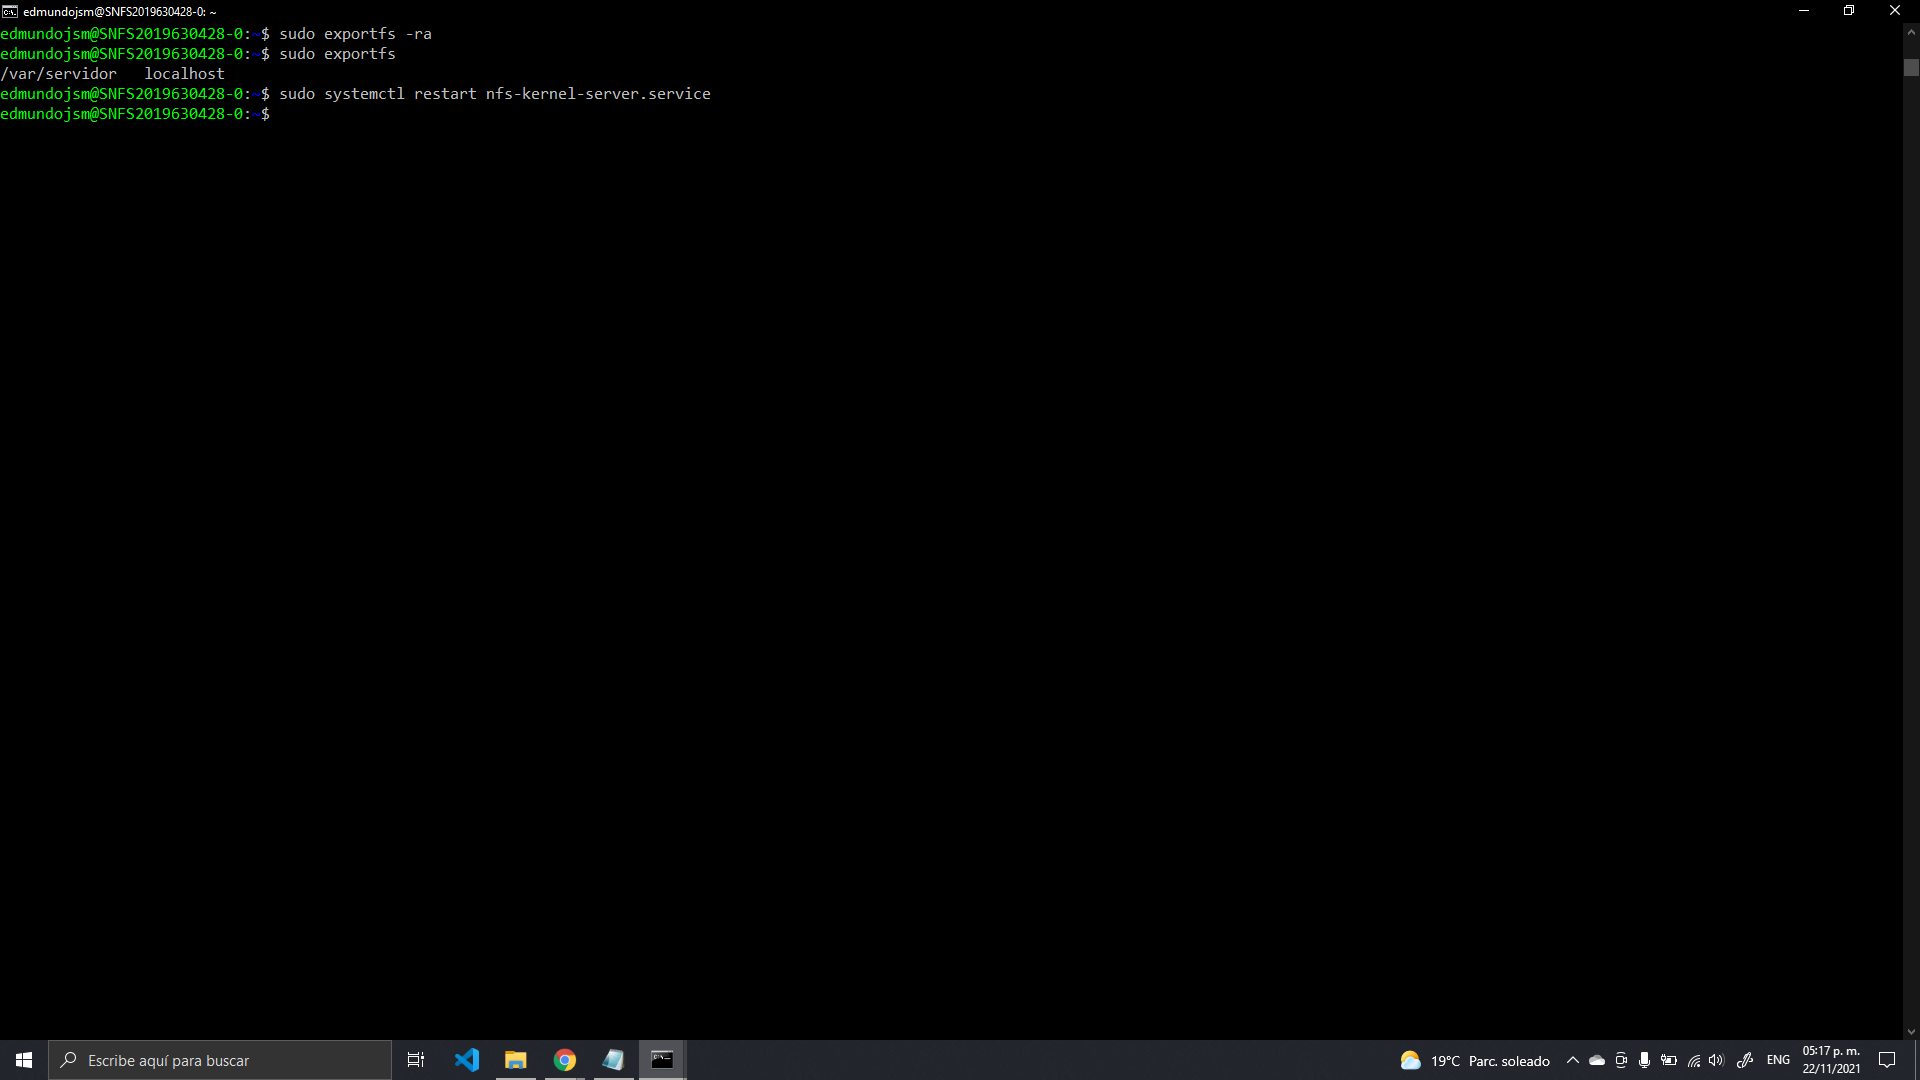
\includegraphics[scale=0.34]{resources/servidor3.png}
			\caption{Punto de montaje en el servidor. Parte 3.}\label{fig:picture}
		\end{figure}	
		\subsection{Punto de montaje en el cliente 1}
		En esta parte veremos todo lo relacionado con la creación del punto de montaje en el cliente 1, es decir, la creación del directorio de montaje y por el momento la conexión inicial SSH entre cliente 1 y servidor y montaje del directorio remoto.
		\begin{figure}[H]
			\centering
			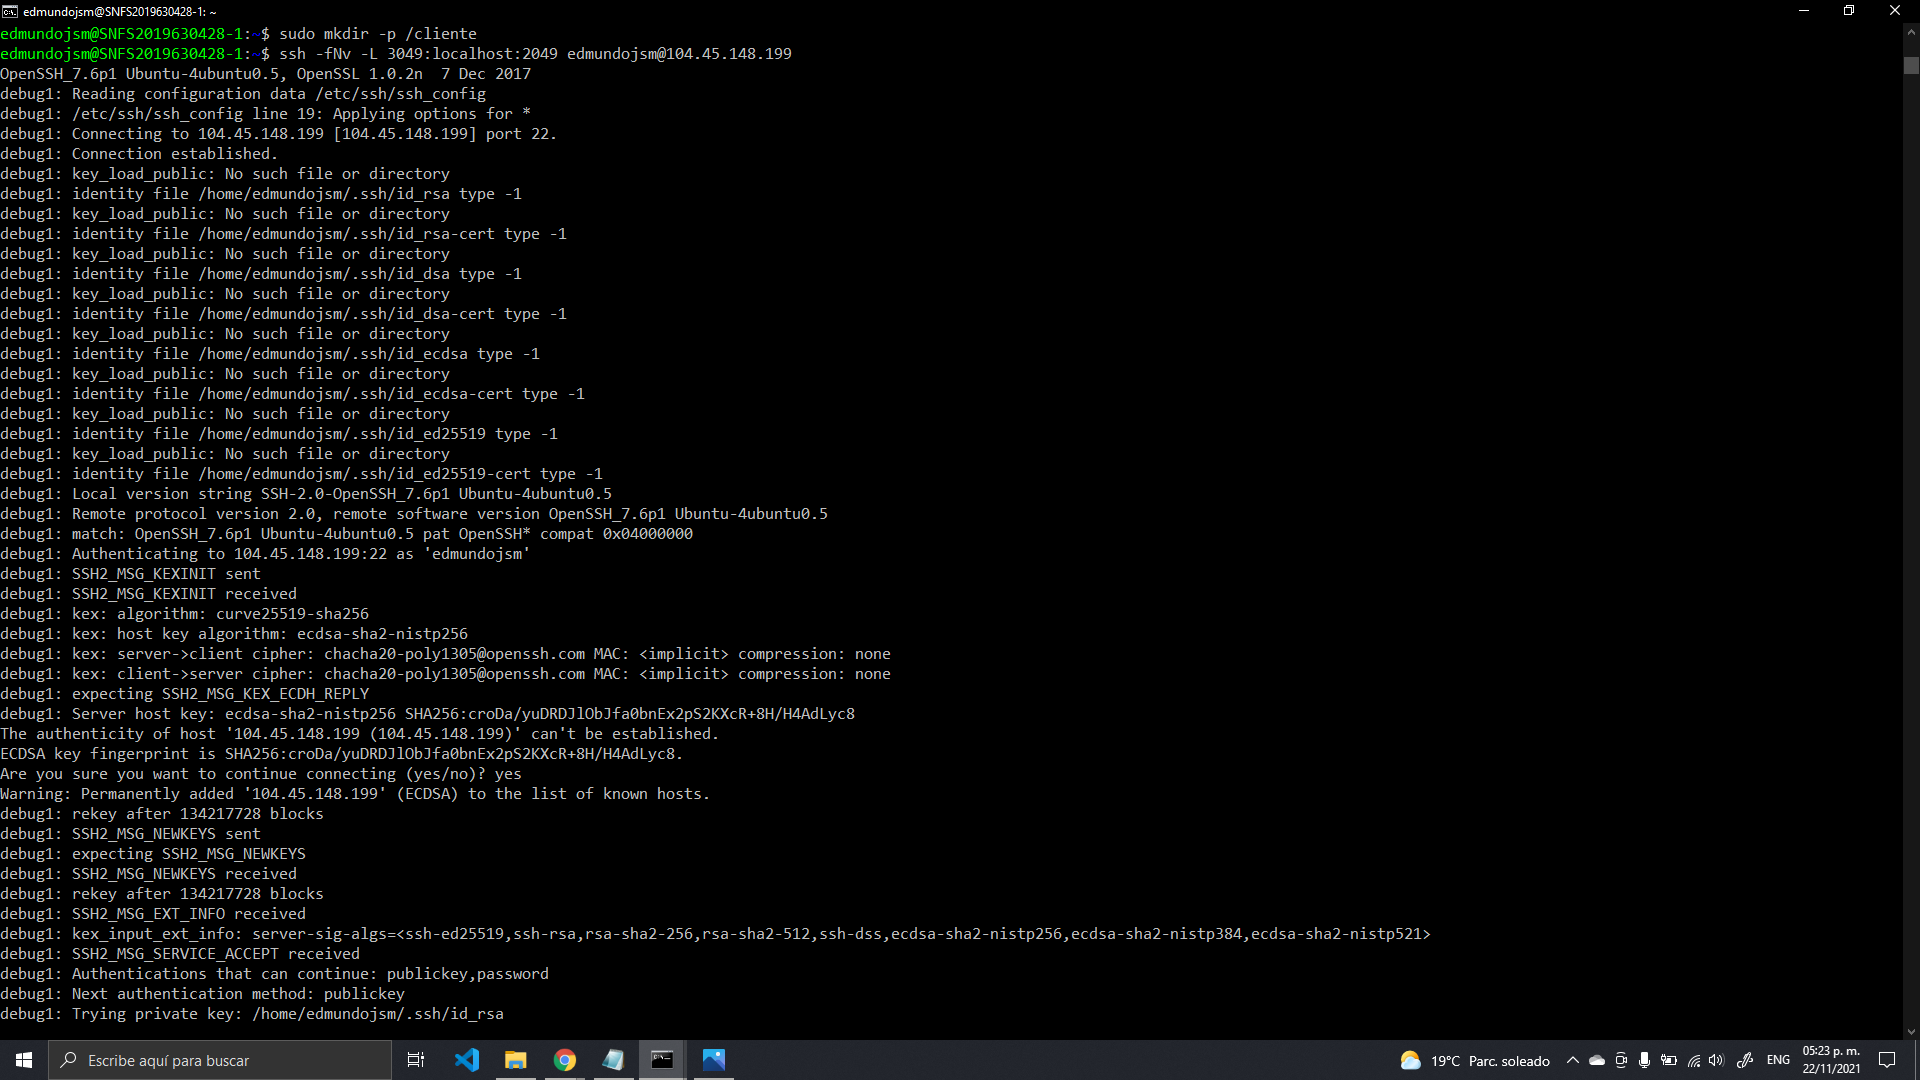
\includegraphics[scale=0.34]{resources/cliente1.1.png}
			\caption{Punto de montaje en el cliente 1. Parte 1.}\label{fig:picture}
		\end{figure}
		\begin{figure}[H]
			\centering
			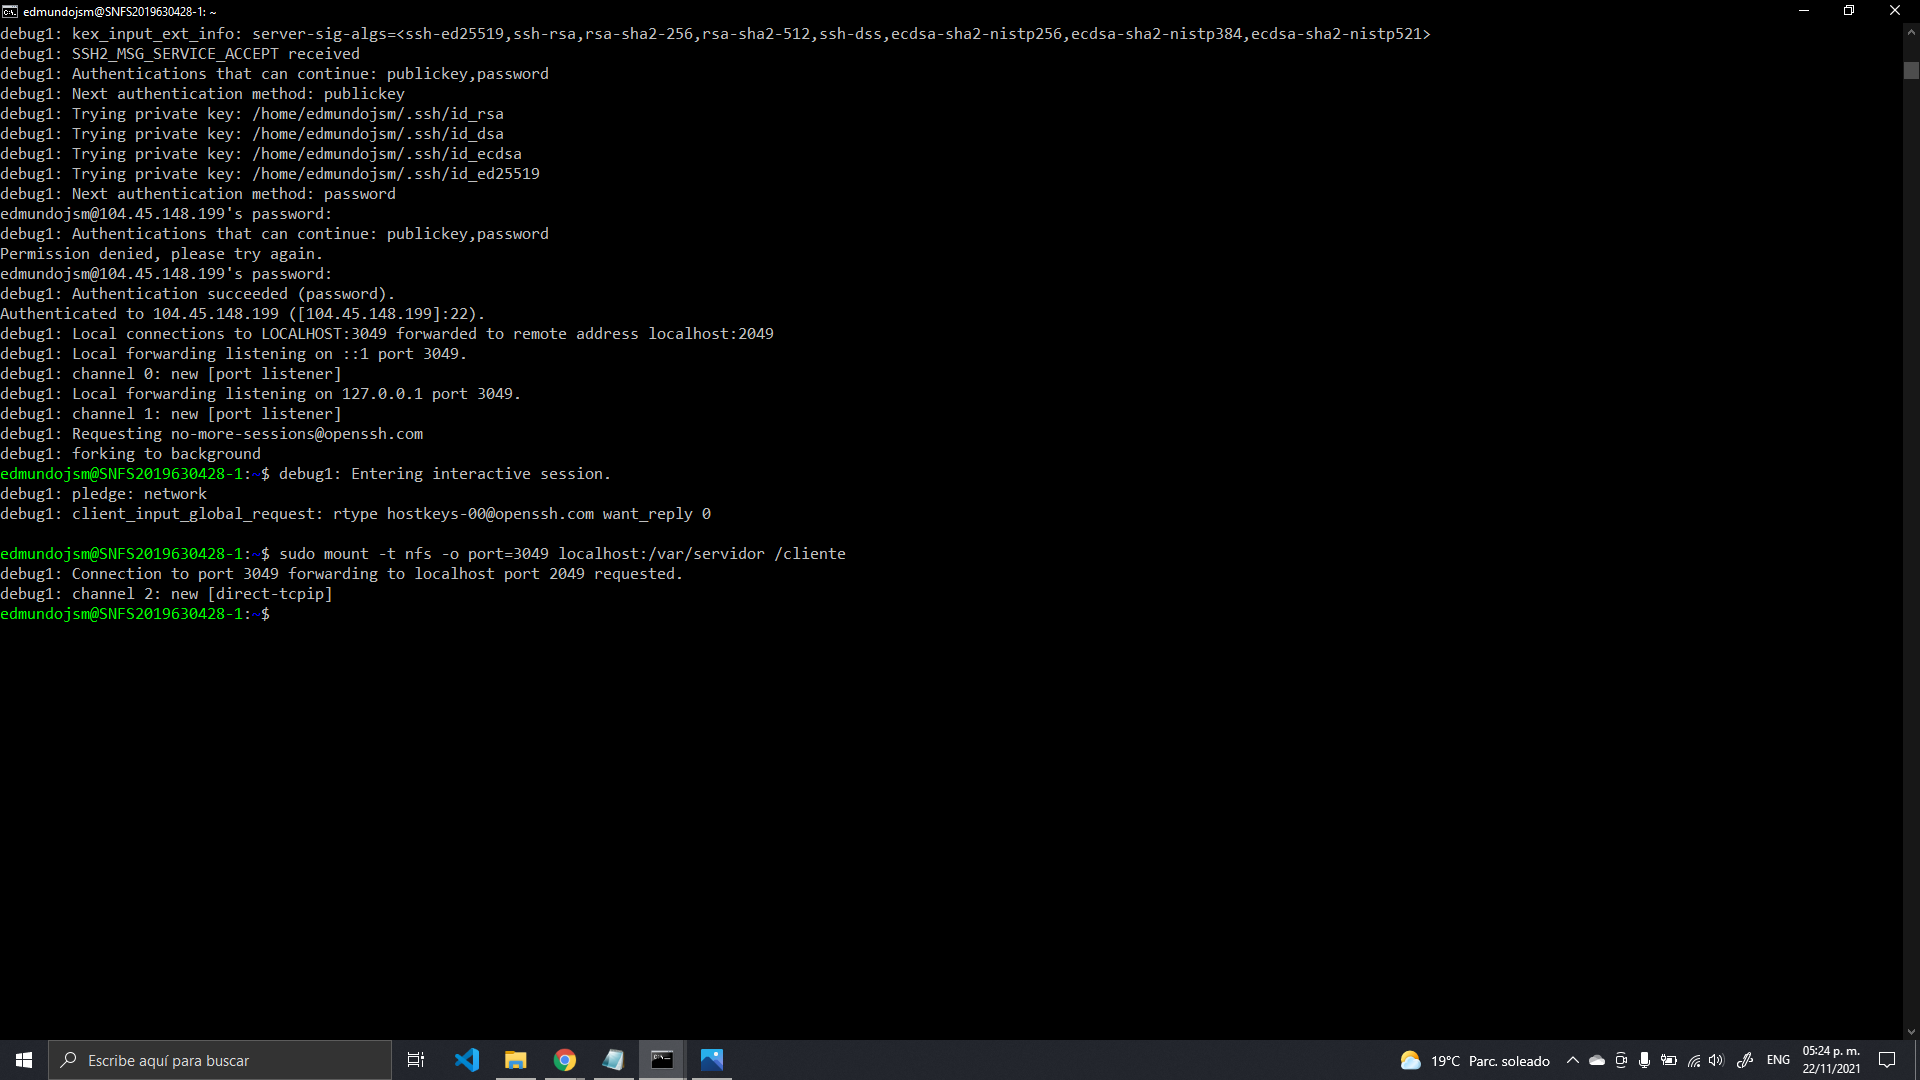
\includegraphics[scale=0.34]{resources/cliente1.2.png}
			\caption{Punto de montaje en el cliente 1. Parte 2.}\label{fig:picture}
		\end{figure}
		\subsection{Punto de montaje en el cliente 2}
		En esta parte veremos todo lo relacionado con la creación del punto de montaje en el cliente 2, es decir, la creación del directorio de montaje y por el momento la conexión inicial SSH entre cliente 1 y servidor y montaje del directorio remoto.
		\begin{figure}[H]
			\centering
			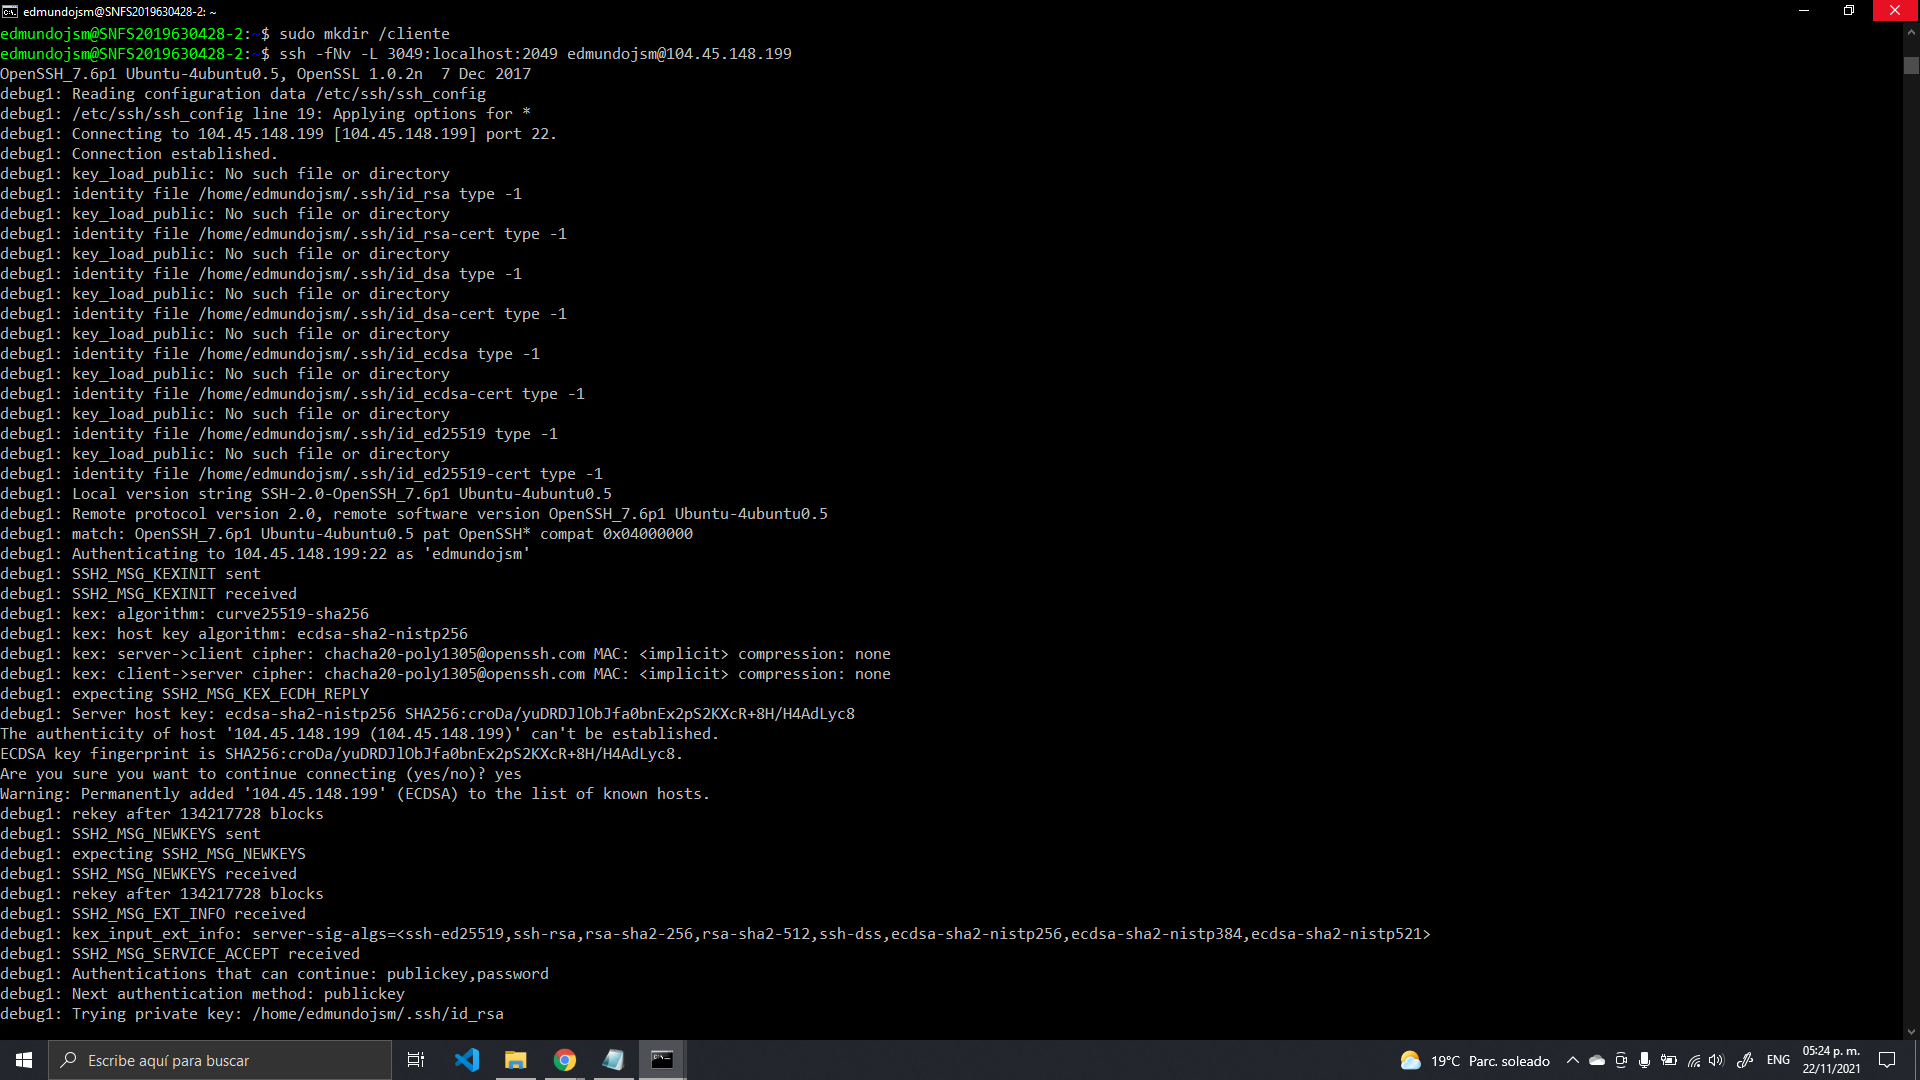
\includegraphics[scale=0.34]{resources/cliente2.1.png}
			\caption{Punto de montaje en el cliente 2. Parte 1.}\label{fig:picture}
		\end{figure}
		\begin{figure}[H]
			\centering
			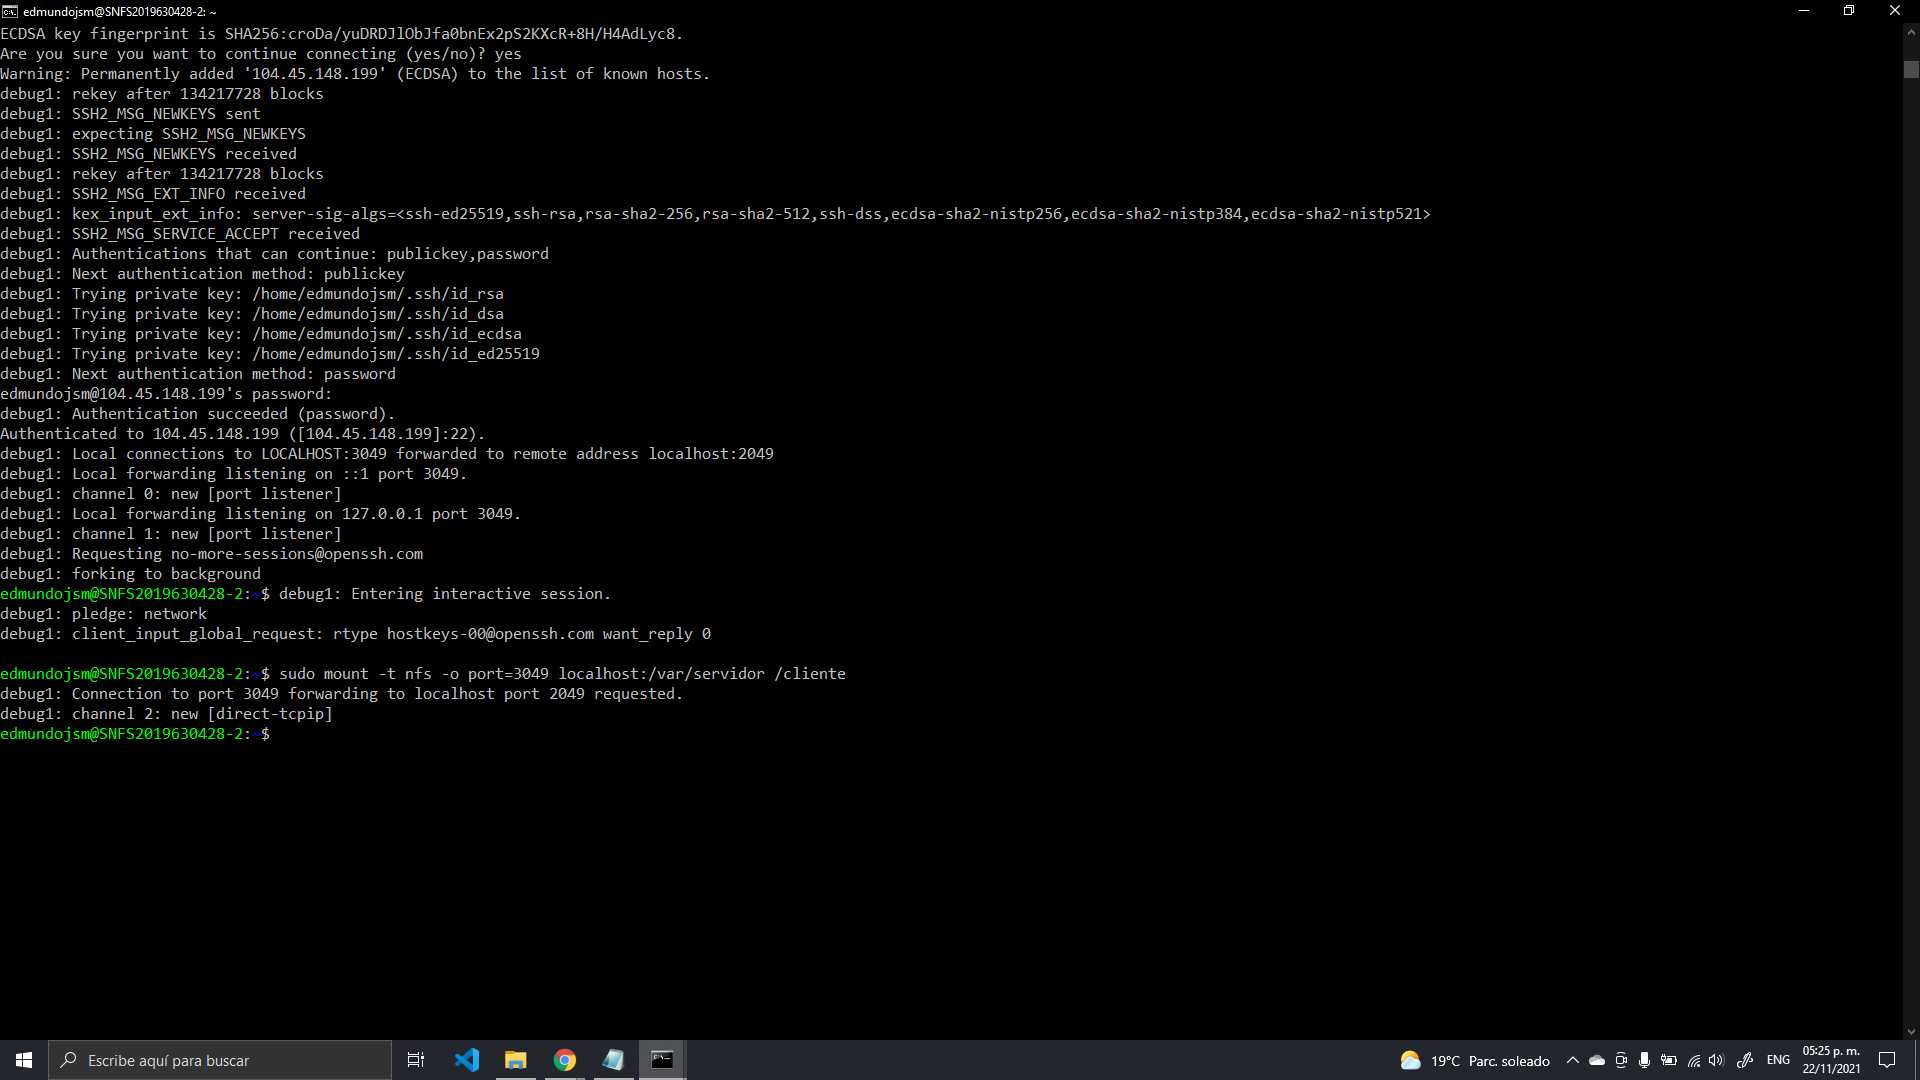
\includegraphics[scale=0.34]{resources/cliente2.2.png}
			\caption{Punto de montaje en el cliente 2. Parte 2.}\label{fig:picture}
		\end{figure}	
	
		\subsection{Creación del archivo de texto con nombre ``archivo.txt'' en el directorio /cliente con el contenido ``esta es una prueba de NFS'' en el cliente 1}
		En esta parte veremos la creación del archivo que usaremos para las pruebas, en este punto lo hacemos en el cliente 1, se creara el archivo con nombre ``archivo.txt'' y con su contenido ``esta es una prueba de NFS'' como podemos ver en la figura 37.
		\begin{figure}[H]
			\centering
			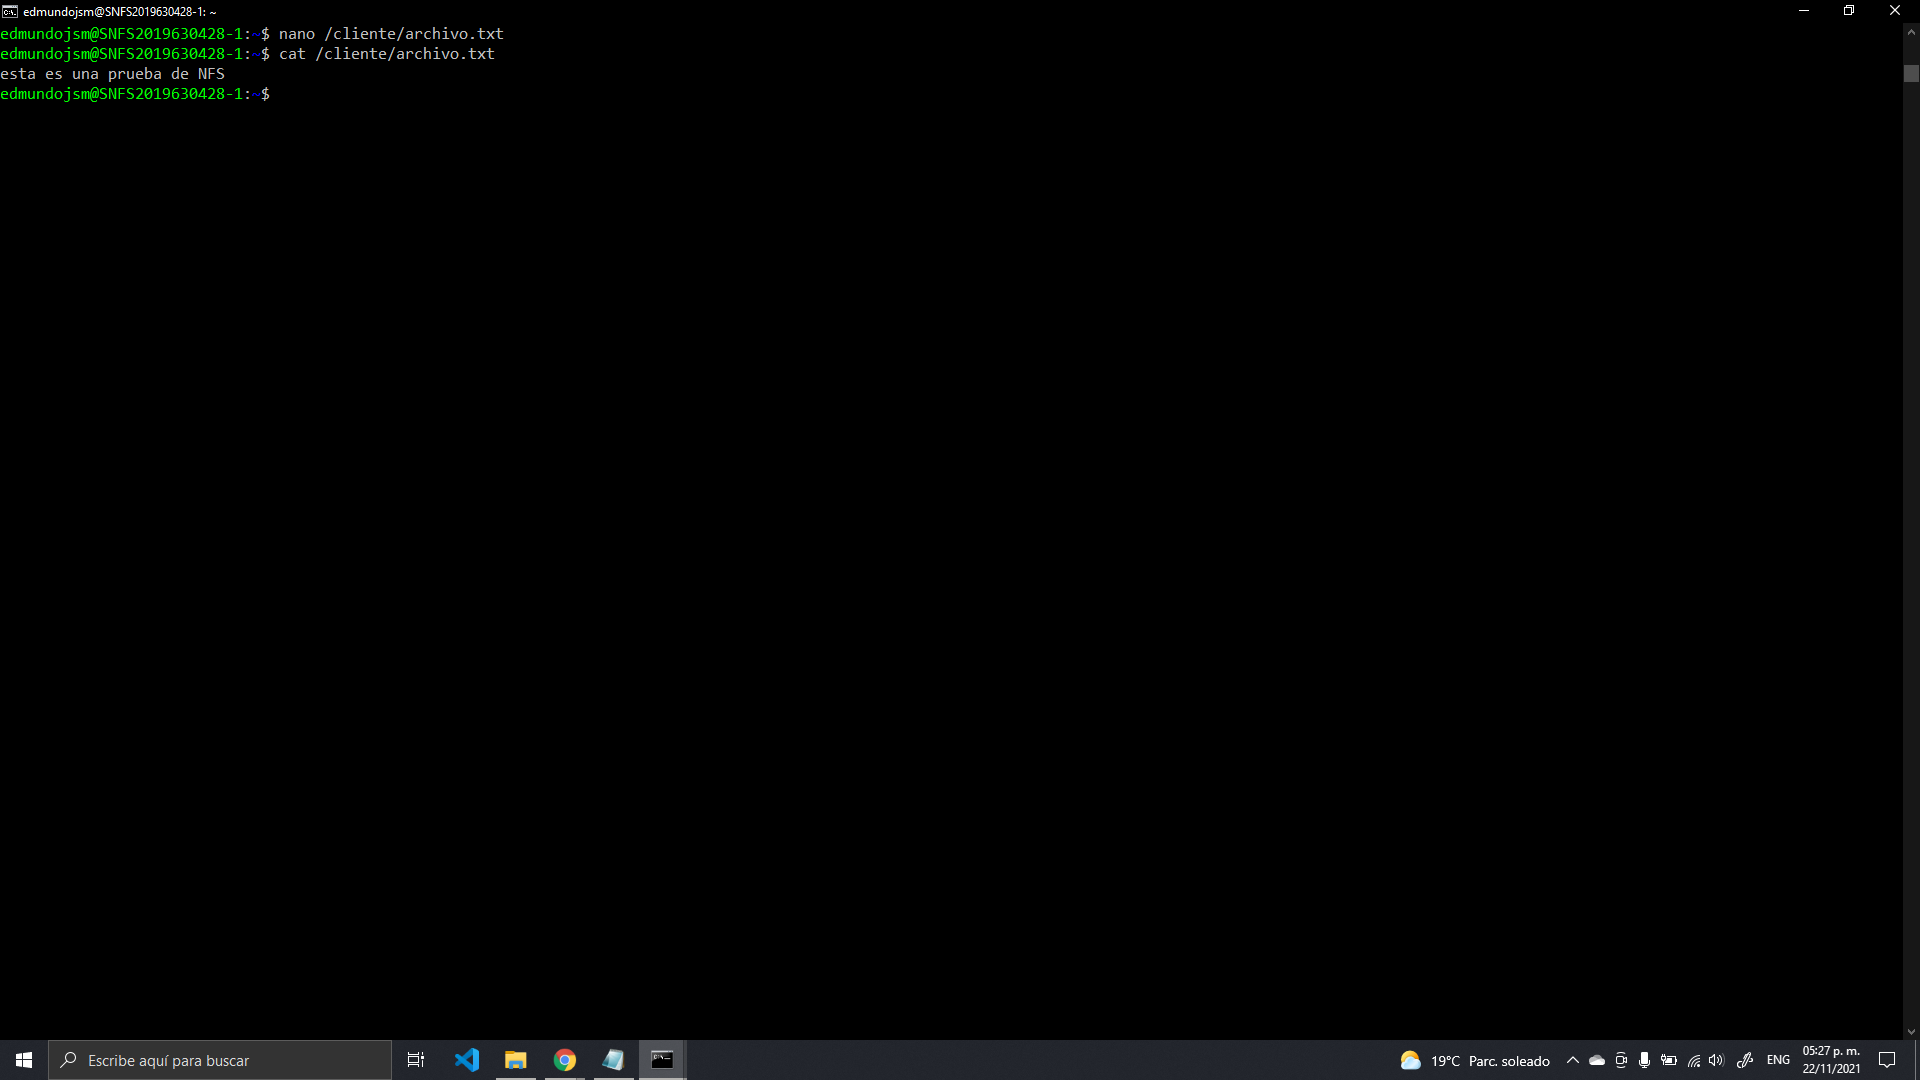
\includegraphics[scale=0.34]{resources/p5y6.png}
			\caption{Creación de archivo y visualizando su contenido.}\label{fig:picture}
		\end{figure}
		\subsection{Desplegado del contenido del archivo cliente/archivo.txt usando ``more'' en el cliente 2}
		En esta parte veremos el desplegado del contenido del archivo creado en el punto anterior en el cliente 2.
		\begin{figure}[H]
			\centering
			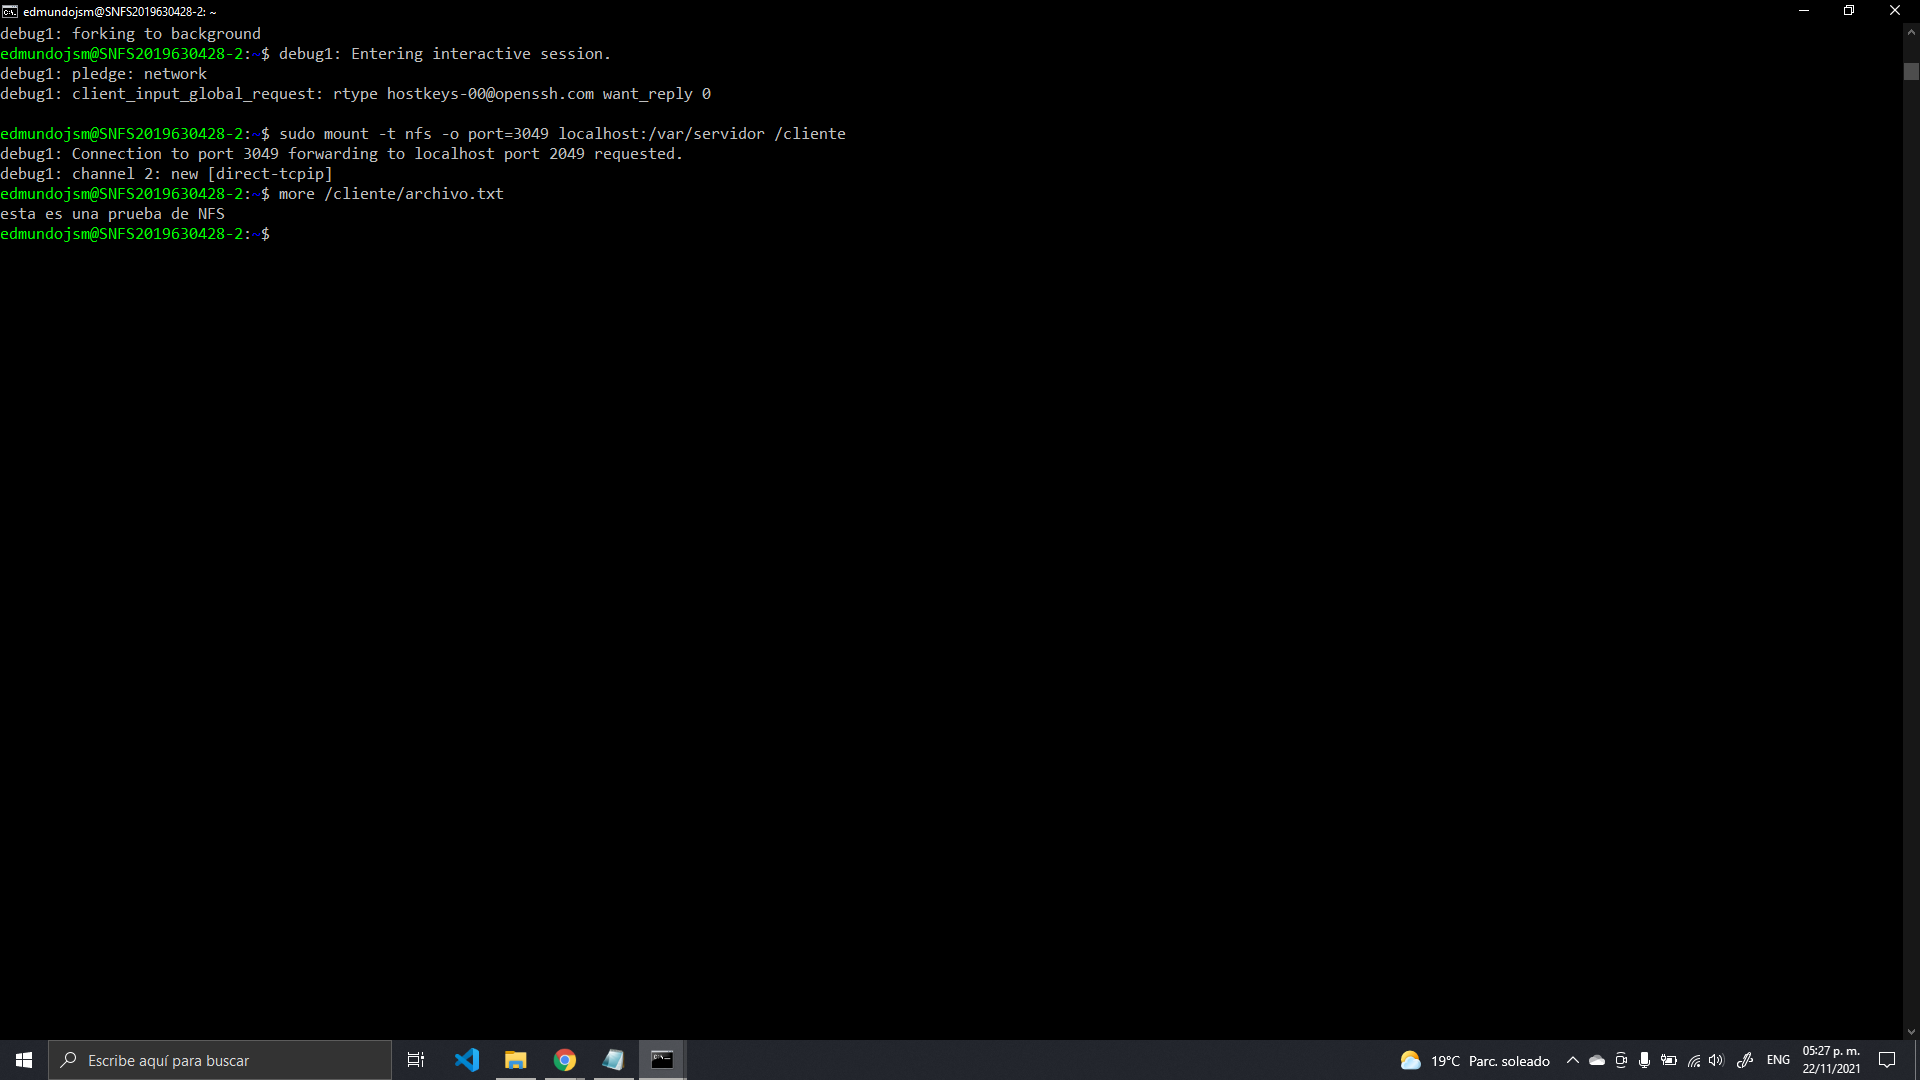
\includegraphics[scale=0.34]{resources/p7.png}
			\caption{Visualización del archivo cliente/archivo.txt usando ``more''.}\label{fig:picture}
		\end{figure}
		\subsection{Configuración necesaria para que inicie NFS al momento de encender la computadora}
		Bueno, sin duda esta es la parte mas complicada de la practica, al inicio pensé que con solo modificar el archivo /etc/fstab como vemos en la primera referencia, sin embargo, esto no nos resulta útil ya que tenemos comunicación por SSH tunneling y aparte el montaje NFS se hace con base en ese túnel. Por lo que reflexionando un poco necesitamos primeramente hacer algo que cree el túnel de manera automática y que se monte NFS justo después de esto, una solución era usar autossh pero este solamente lo hace mientras se este activo y no funciona si se hace un reboot o un apagado y encendido de la maquina ya sea virtual o física (esto con sistema operativo Linux) y el hacer el montaje justo después de esto no se solucionaba, por lo que recordando un materia que tengo inscrita actualmente decidí hacer uso de demonios, en resumen los demonios en Linux es un programa no interactivo (es decir, que el usuario no puede controlar directamente) que se encarga de procesos del sistema en un segundo plano, la creación de ellos es muy sencilla y solo ocupamos hacer uso de sudo, es importante recordar un poco sobre Linux y es que tenemos principalmente dos tipos de administradores de sistema, el mas usual y típico es systemd el cual es que encontraremos la mayor cantidad de veces para este los demonios tienen una extension .service, pero también tenemos System V el cual tiene como extension .sysv para esta practica hacemos uso de systemd por lo que los scripts creados funcionaran solamente para systemd. Con lo anterior tenemos solucionado la creación del túnel SSH usando demonios y autossh para asegurar que funcione todo el tiempo y tenemos parcialmente solucionado el montaje ya que necesitamos ejecutar un comando que veremos posteriormente, por lo que necesitamos hacer uso de un script en shell.\par
		Shell es un ejecutable con extension .sh en sistema Unix el cual permite ejecutar comandos que sean escritos en este no importando que comando sea, sin embargo, para poder hacer uso de un archivo .sh necesitamos que se ejecute por la interfaz de usuario bash que veremos mas adelante ya que esta es una pequeña introducción. Ahora si vayamos a la creación, ejecución y pruebas del funcionamiento de los demonios.
		\subsubsection{Preparación del cliente 1 antes de crear y usar los demonios}
		En esta parte necesitamos preparar a la maquina virtual en este caso el cliente 1 con la creación de llaves para conexión ssh esto mediante el comando ssh-keygen, en esta ocasión vamos a usar RSA de 2048 bits como vemos en la figura 39 nos solicita nombrar a nuestra llave, en este caso se llama ``cliente1'' y nos pregunta por una frase la cual es para dar mayor seguridad a las claves pero para esta ocasión la omitiremos, una vez finalizado el comando vemos que nos generan dos archivos ``cliente1'' y ``cliente1.pub'', necesitamos hacer una copia de ``cliente1'' y darle la extension pem por lo que ahora tenemos un archivo extra con nombre ``cliente1.pem'' el cual nos sera útil para el demonio del tunel. Finalmente necesitamos copiar la llave al servidor mediante ssh-copy-id pasando como parámetro el archivo cliente.pub y hacia que servidor con el usuario se enviara, evidentemente nos pedirá la contraseña.
		\begin{figure}[H]
			\centering
			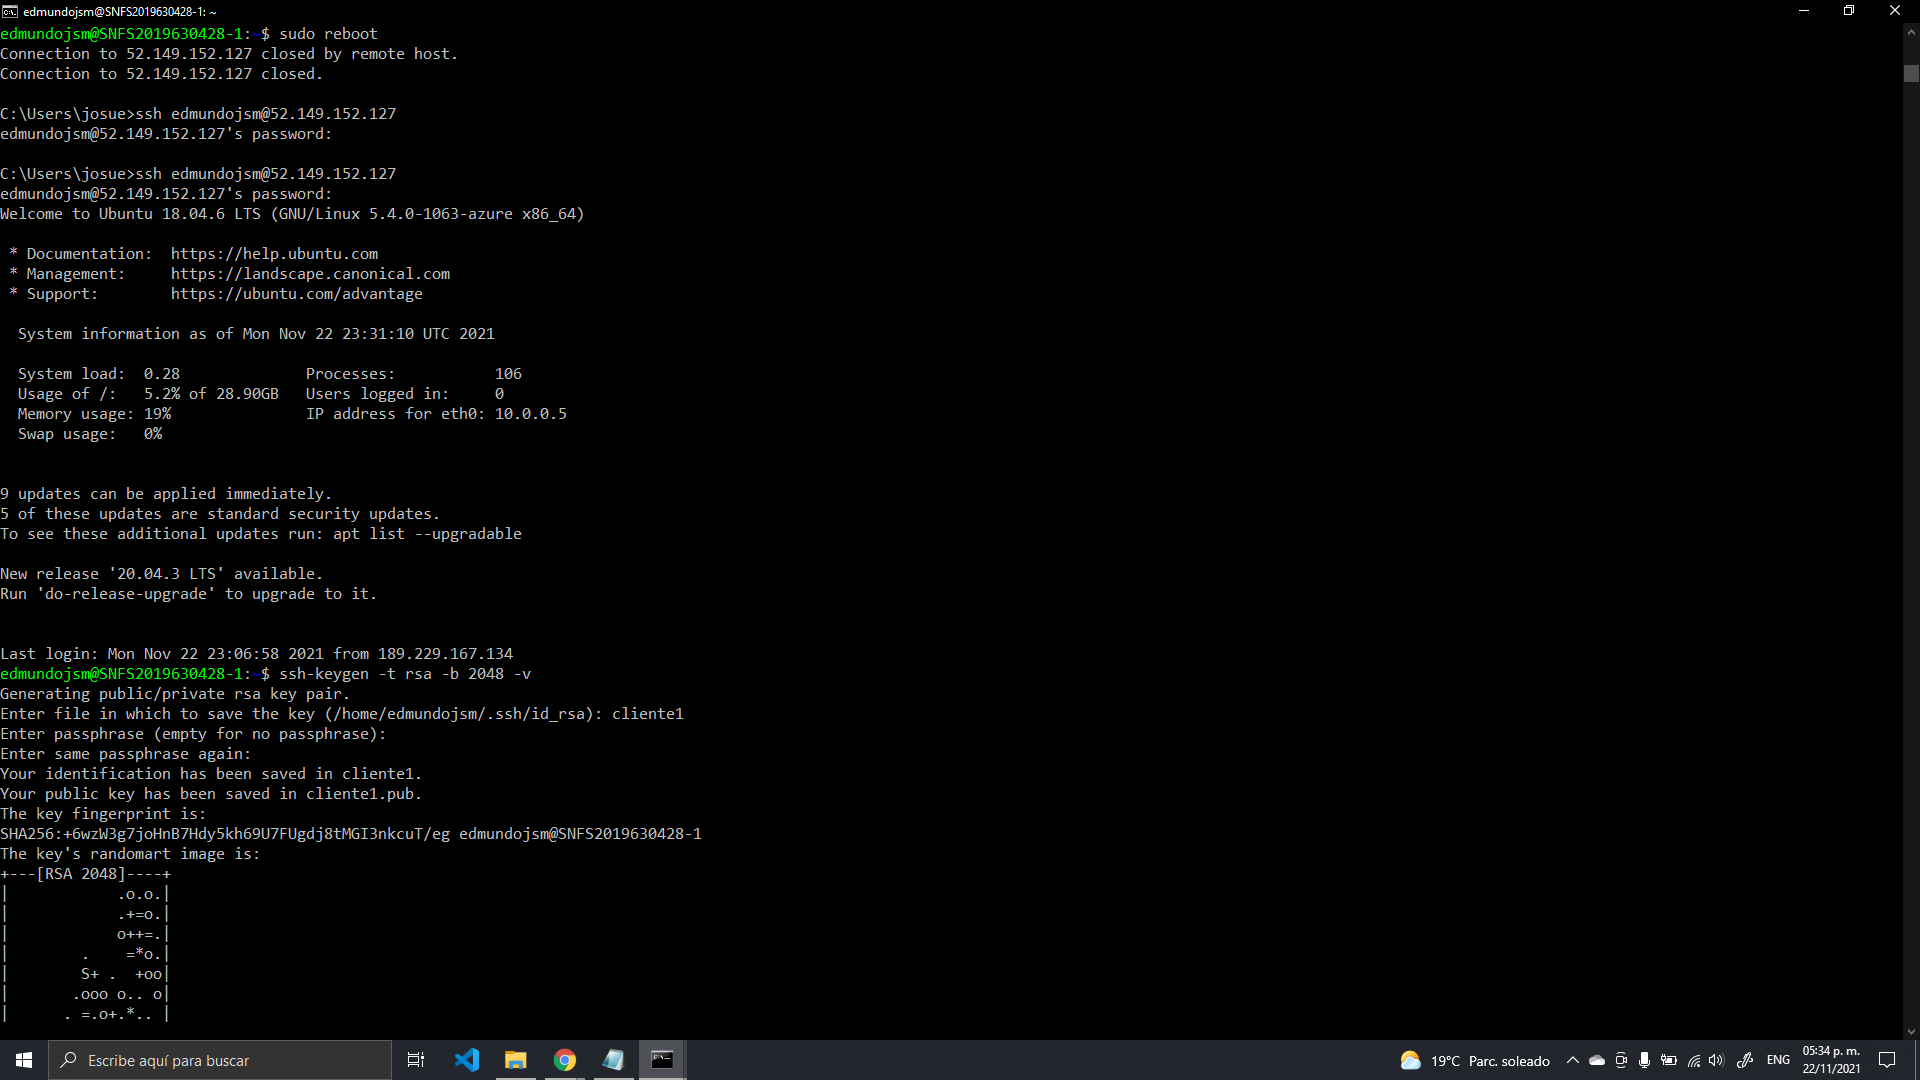
\includegraphics[scale=0.34]{resources/preparacionCliente1.1.png}
			\caption{Preparación del cliente 1. Parte 1.}\label{fig:picture}
		\end{figure}
		\begin{figure}[H]
			\centering
			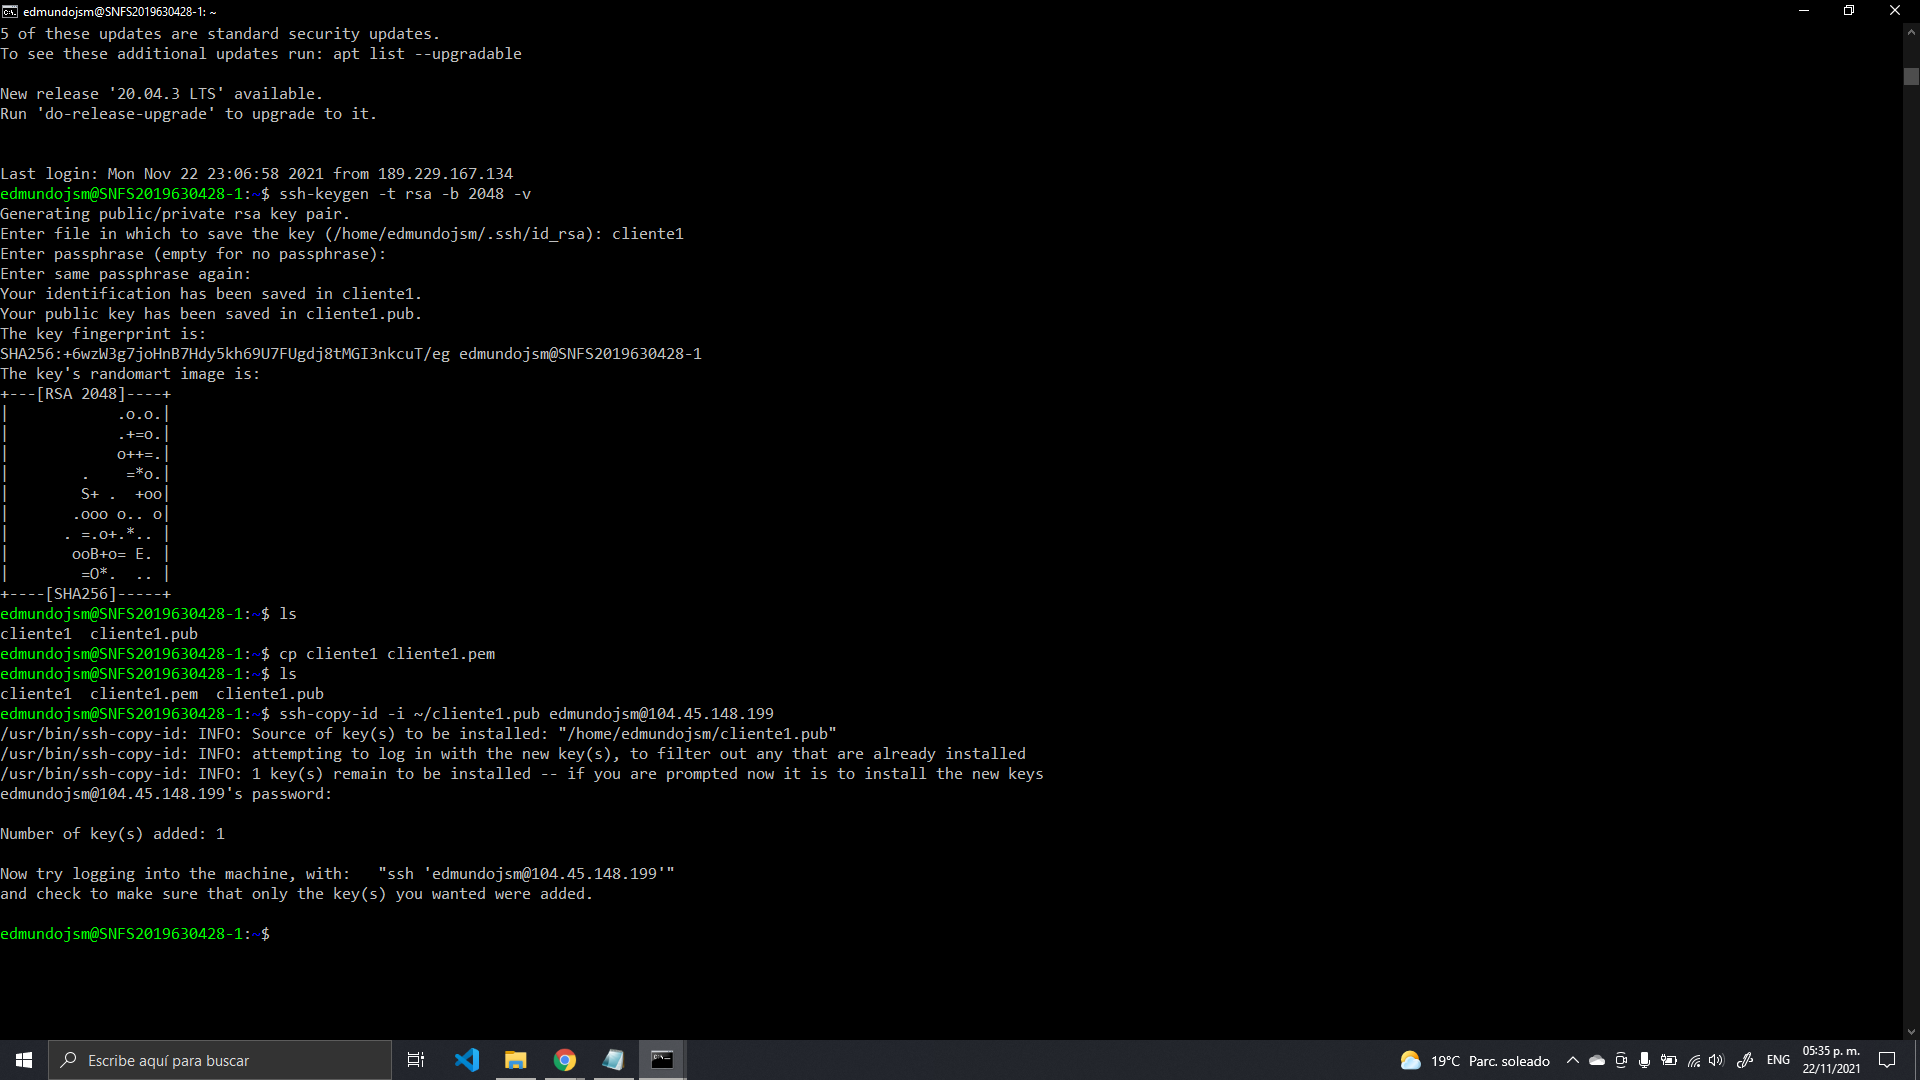
\includegraphics[scale=0.34]{resources/preparacionCliente1.2.png}
			\caption{Preparación del cliente 1. Parte 2.}\label{fig:picture}
		\end{figure}
		\subsubsection{Preparación del cliente 2 antes de crear y usar los demonios}
		En esta parte repetimos lo que se vio en el punto anterior pero ahora las llaves llevan como nombre ``cliente2''.
		\begin{figure}[H]
			\centering
			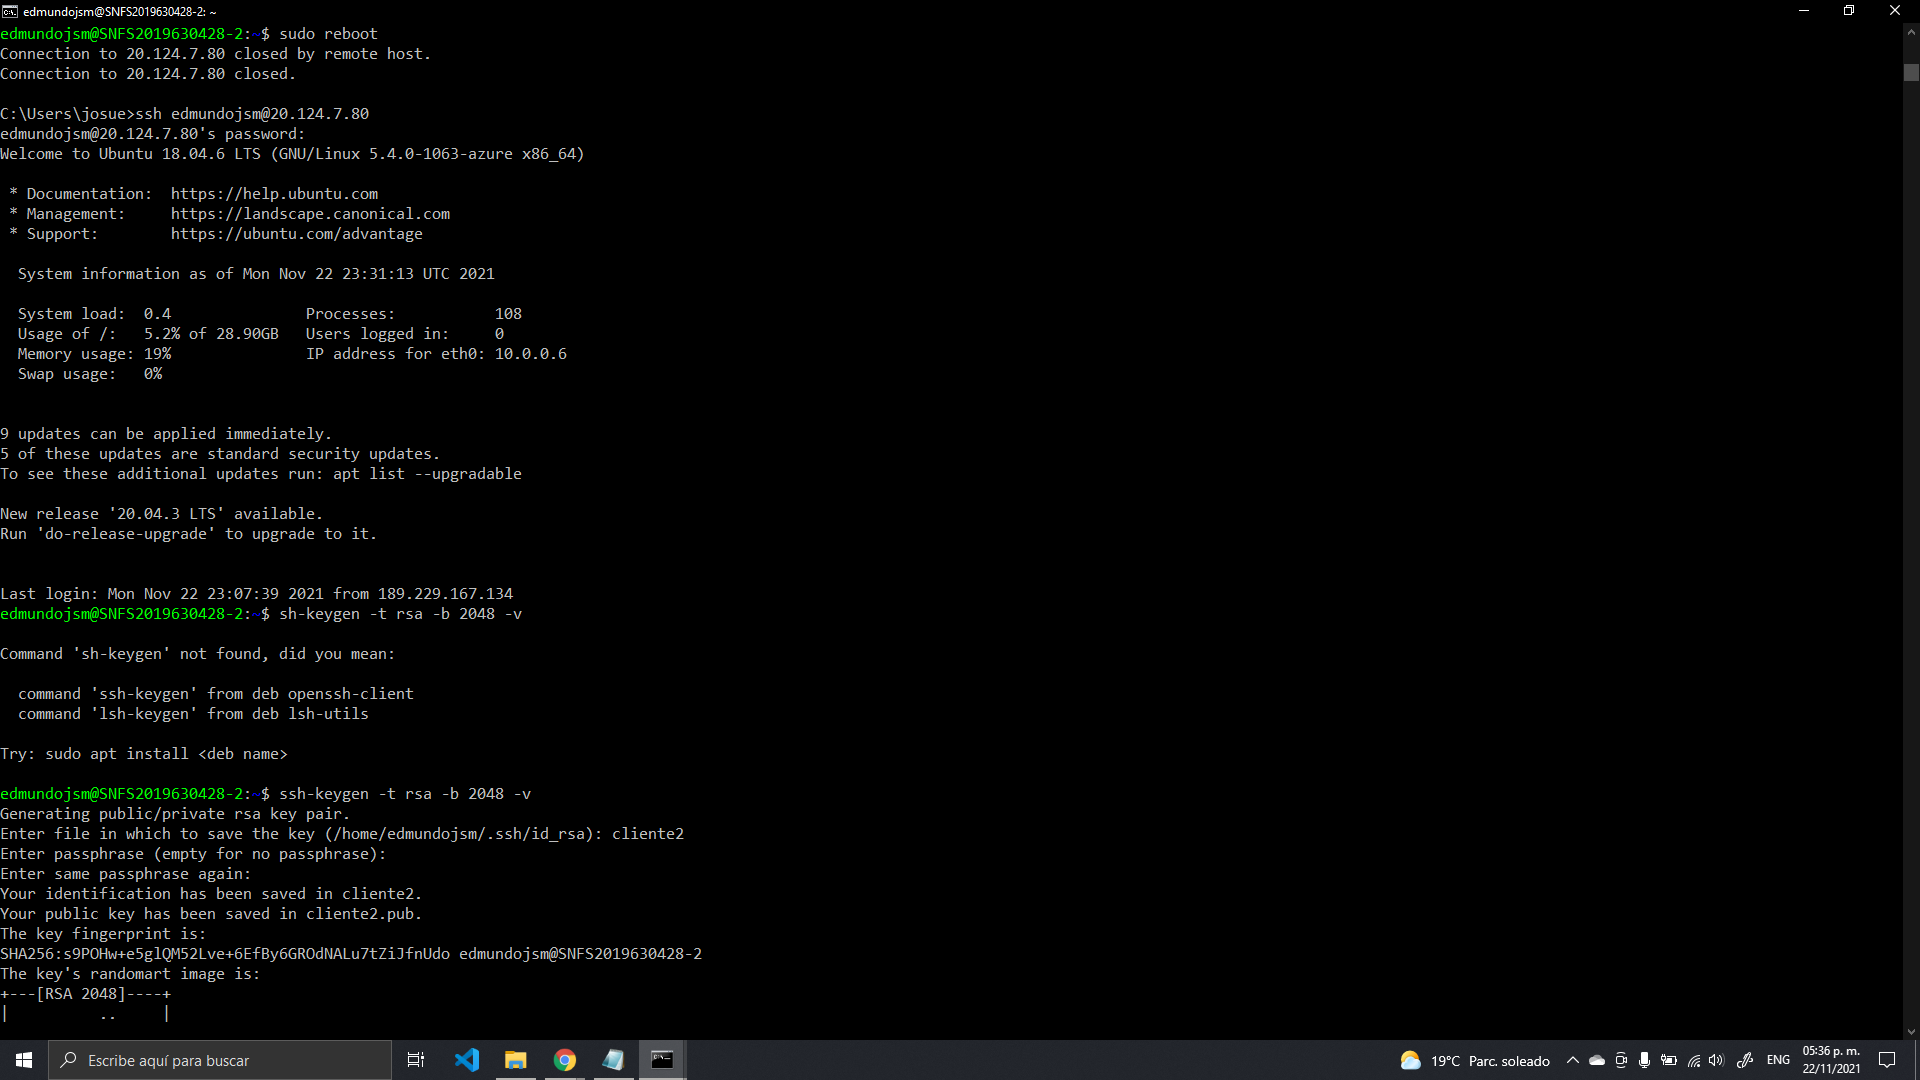
\includegraphics[scale=0.34]{resources/preparacionCliente2.1.png}
			\caption{Preparación del cliente 2. Parte 1.}\label{fig:picture}
		\end{figure}
		\begin{figure}[H]
			\centering
			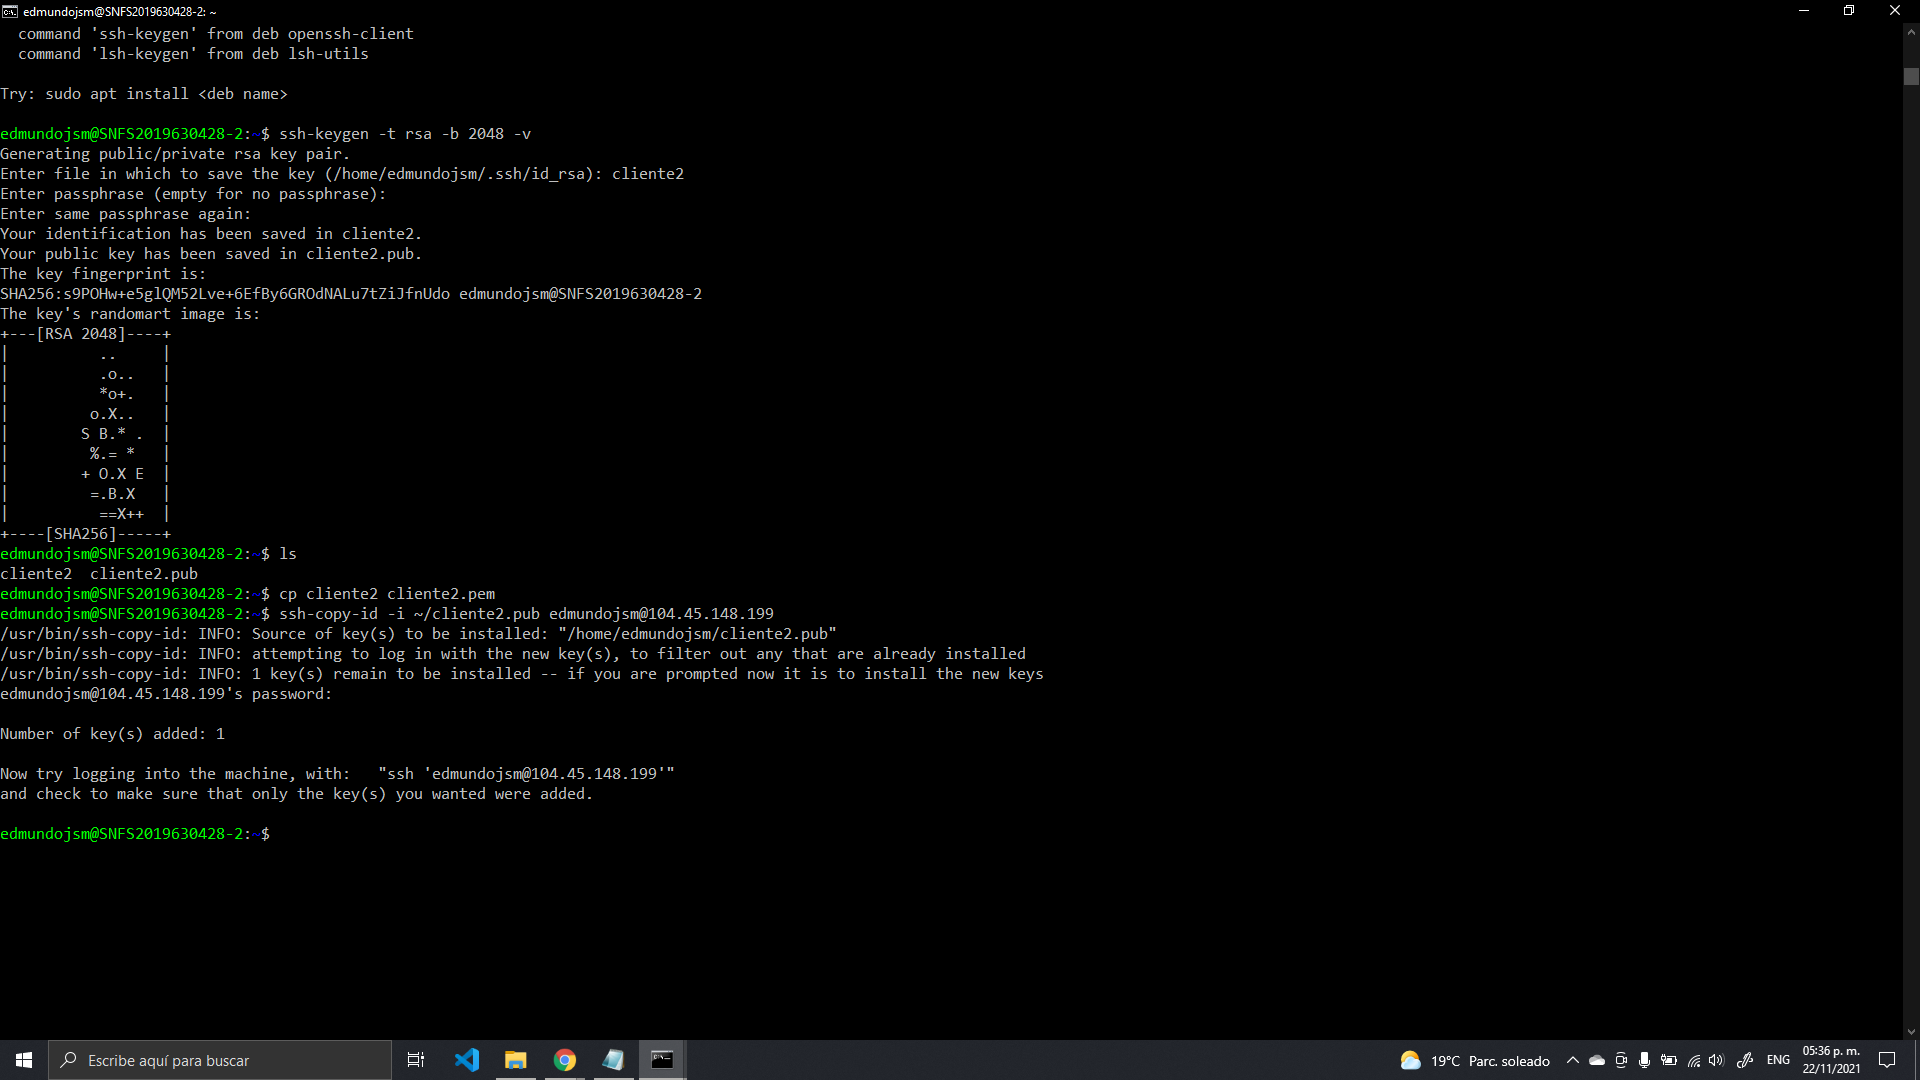
\includegraphics[scale=0.34]{resources/preparacionCliente2.2.png}
			\caption{Preparación del cliente 2. Parte 2.}\label{fig:picture}
		\end{figure}
		\subsubsection{Comprobación de que las llaves se copiaron al servidor correctamente }
		En esta parte veremos el contenido del archivo  /.ssh/authorized\_keys. y como vemos en la figura 43 nos muestra las llaves cifradas y a quien pertenece cada una por lo que podemos decir que fue un éxito este proceso.
		\begin{figure}[H]
			\centering
			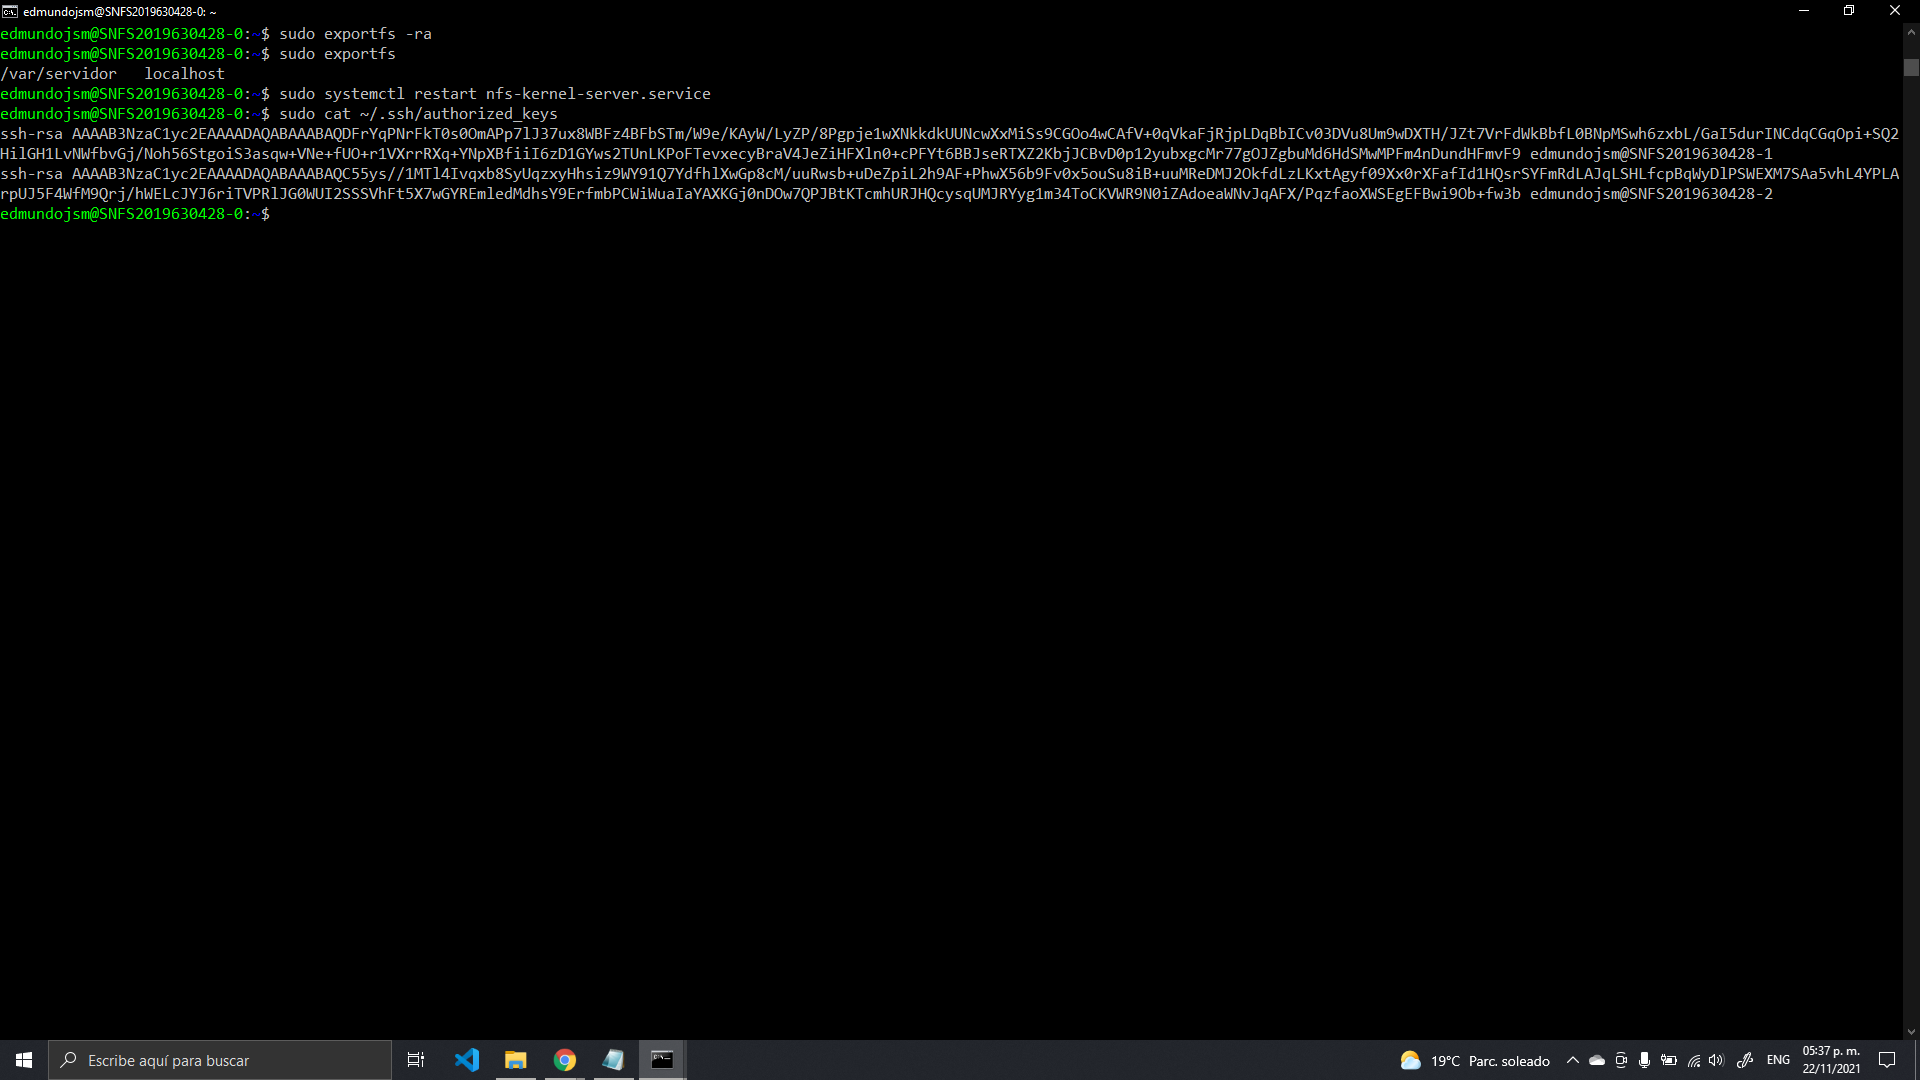
\includegraphics[scale=0.34]{resources/llavesok.png}
			\caption{Llaves copiadas con éxito en el servidor.}\label{fig:picture}
		\end{figure}
		Una vez preparado los clientes vayamos directo a los demonio que es donde esta lo mas complicado y pesado de esto, mencionar que esto lo veremos detalladamente con el cliente 1 pero con el cliente 2 solo se mostraran las imágenes ya que es exactamente el mismo proceso.
		\subsubsection{Creación de los demonios en el cliente 1 }
		Ahora creamos lo que comentamos al inicio de esta sección y es que creamos dos .service (serán dos demonios) y un script en shell, estos tienen los nombre autossh-tunel.service, montaje-nfs.service y nfsmount.sh y si vemos la sigiuiente figura podemos ver el contenido de cada uno de estos
		\begin{figure}[H]
			\centering
			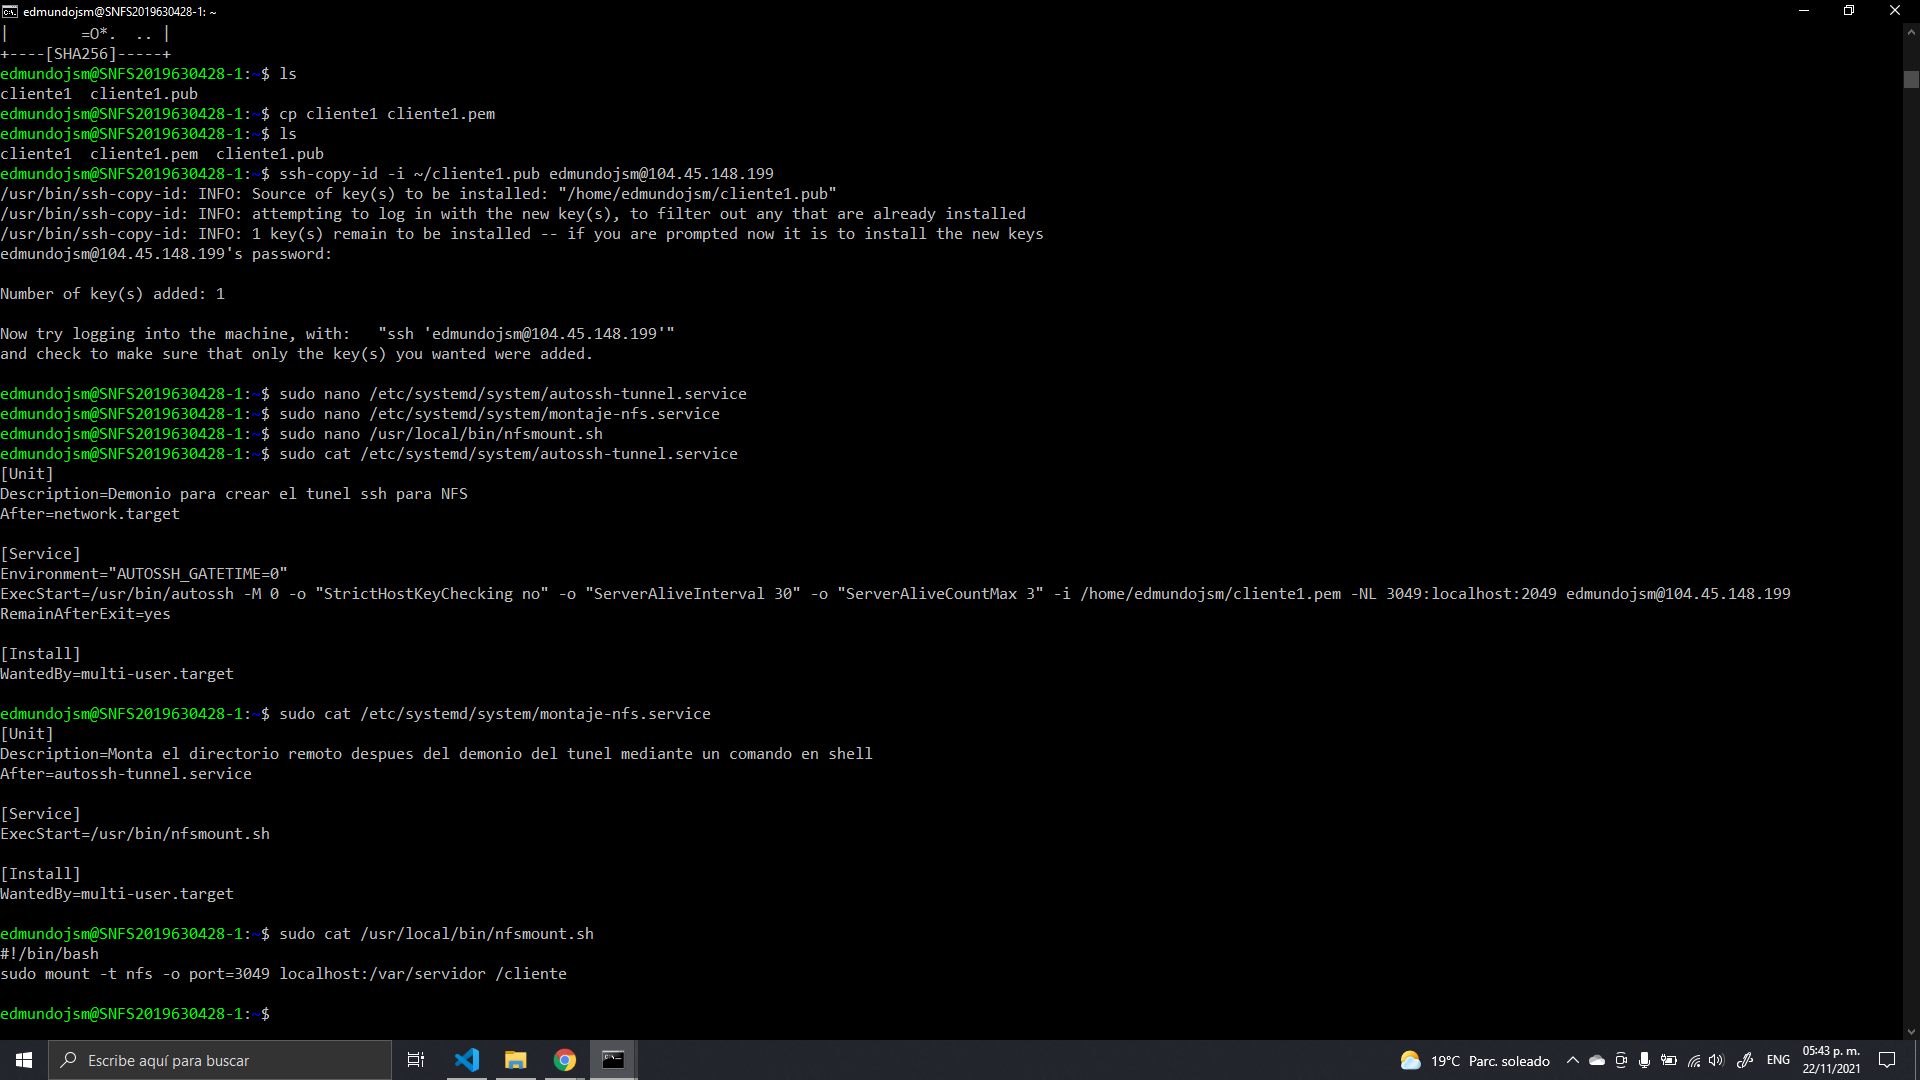
\includegraphics[scale=0.34]{resources/demonioc1.png}
			\caption{Creación de demonio y script en shell para el cliente 1.}\label{fig:picture}
		\end{figure}
		Sin embargo a continuación dejo el esqueleto para poder crear demonios con el mismo fin pero en diferentes maquinas o con diferente servidor, mencionar que se pudo crear un solo demonio y que este se encargue de ejecutar todo pero es mejor tener separado los demonios, esto con el fin de saber que demonio fue el que fallo.\par
		Demonio para crear el tunel ssh (autossh-tunel.service)
		\begin{verbatim}
			[Unit]
Description=Demonio para crear el tunel ssh para NFS
After=network.target

[Service]
Environment="AUTOSSH_GATETIME=0"
ExecStart=/usr/bin/autossh -M 0 -o "StrictHostKeyChecking no" -o "ServerAliveInterval 30" 
-o "ServerAliveCountMax 3" -i <ubicación de llave con extension .pem> -NL 
<puerto local del cliente>:localhost:<puerto del servidor> <usuario>@<IP del servidor>
RemainAfterExit=yes

[Install]
WantedBy=multi-user.target

		\end{verbatim}
		Demonio para montar el directorio remoto (montaje-nfs.service), mencionar que para este caso se aconseja tener el script en shell en /usr/local/bin/ ya que es ahí en donde Linux tiene guardado todos los script en shell que utiliza y todos los usuarios lo pueden usar, también comentar que la instrucción After es para que se ejecute después de un demonio, en este caso después de nuestro demonio del tunel ssh, mencionar que aquí yo cometí un error en la ruta que puse al inicio y que por eso sale un mensaje de error que veremos posteriormente pero que cambiamos el archivo y la ruta y se soluciona, esto en las próximas figuras.
		\begin{verbatim}
[Unit]
Description=Monta el directorio remoto despues del demonio del tunel
After=autossh-tunnel.service

[Service]
ExecStart= <Ruta absoluta del script en shell>

[Install]
WantedBy=multi-user.target
		\end{verbatim}
		Finalmente el script en shell, es necesario poner la primera linea para que se ejecute en bash, en caso contrario no funcionara.
		\begin{verbatim}
#!/bin/bash
sudo mount -t nfs -o port=3049 localhost:/var/nfs /nfs
		\end{verbatim}
		Ahora veamos la correccion de ruta que se hizo para el demonio del montaje de nfs, solo se cambia la ruta, fue un error mio, mencionar que me di cuenta al probarlo por eso en el prompt veremos un error pero después de corregirlo funciona de manera correcta.
		\begin{figure}[H]
			\centering
			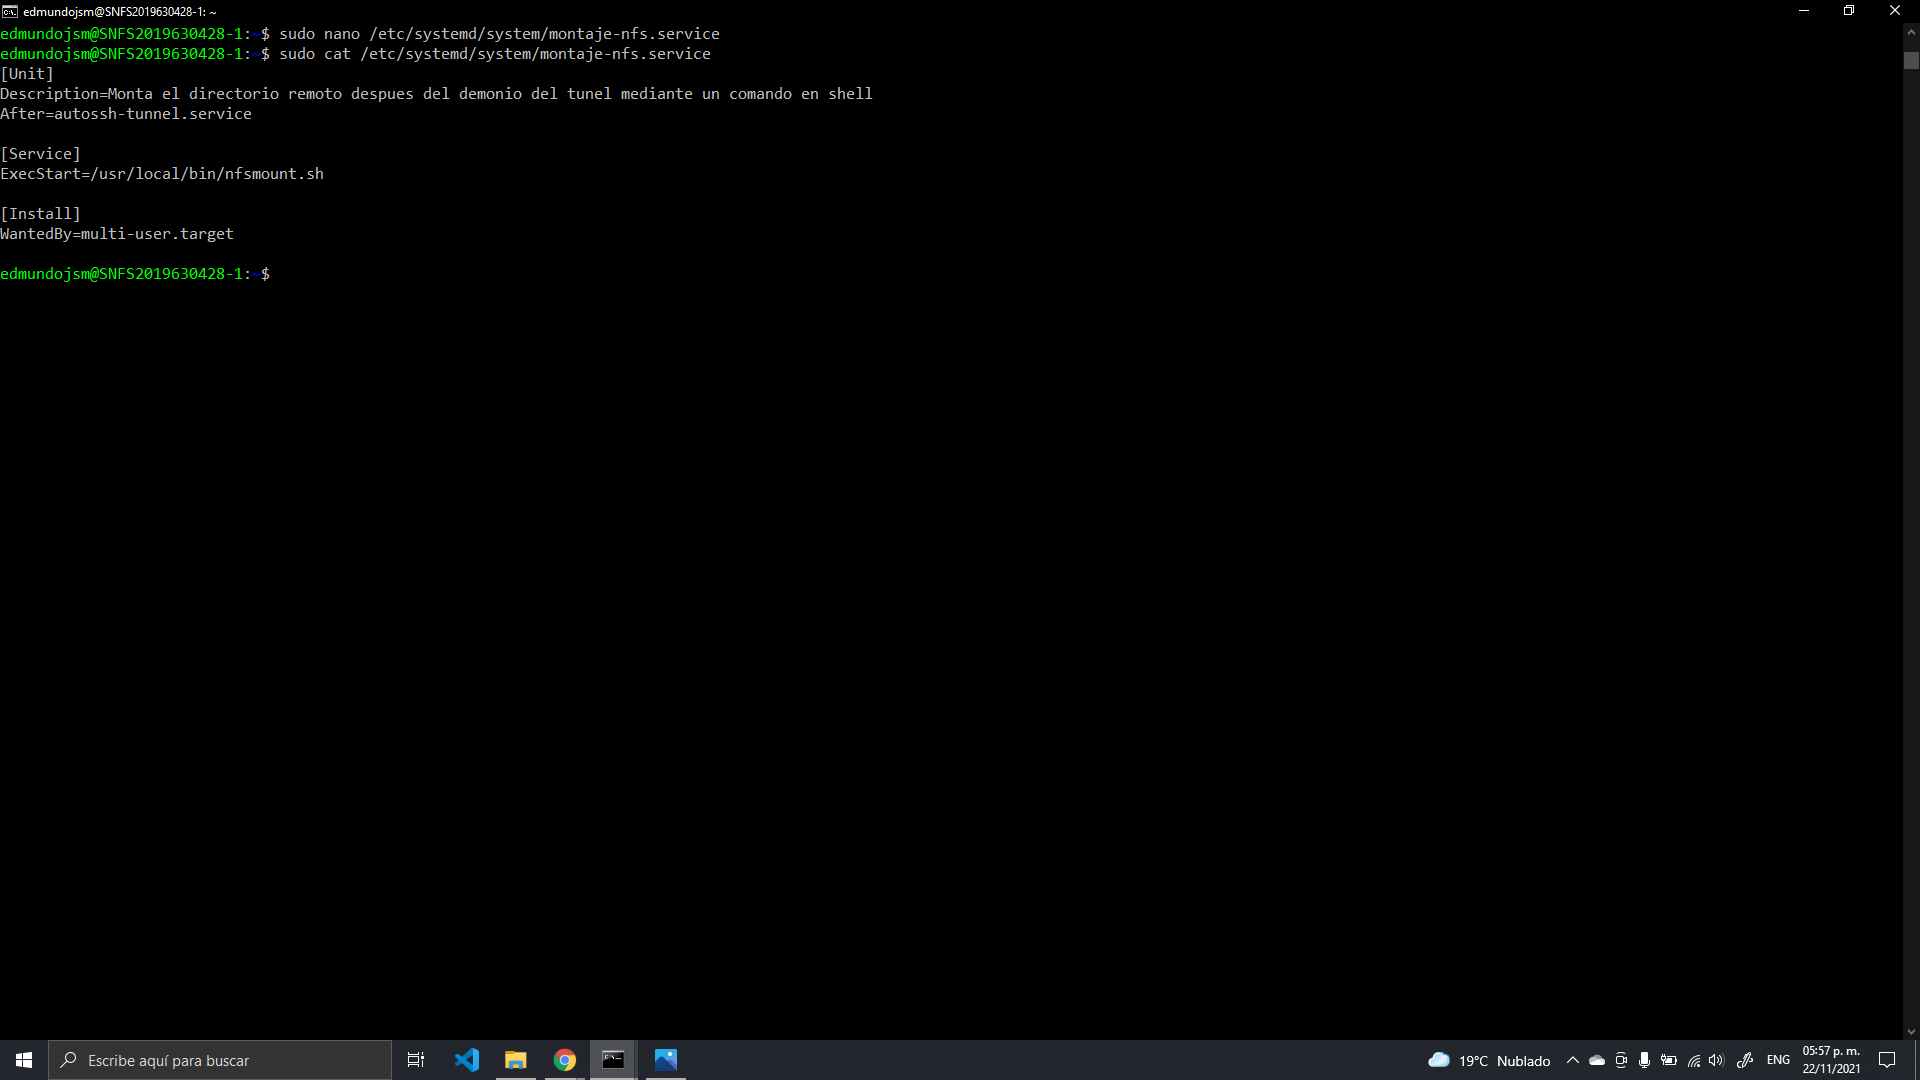
\includegraphics[scale=0.34]{resources/demonioc1actu.png}
			\caption{Actualización en la ruta del script en shell.}\label{fig:picture}
		\end{figure}
		 Y como vemos en la figura siguiente los demonios hacen su función y se ejecutan correctamente, mencionar que al ver el status del demonio del montaje nos dice en donde esta el error y por eso es una buena opción usar demonios separados
		 \begin{figure}[H]
			\centering
			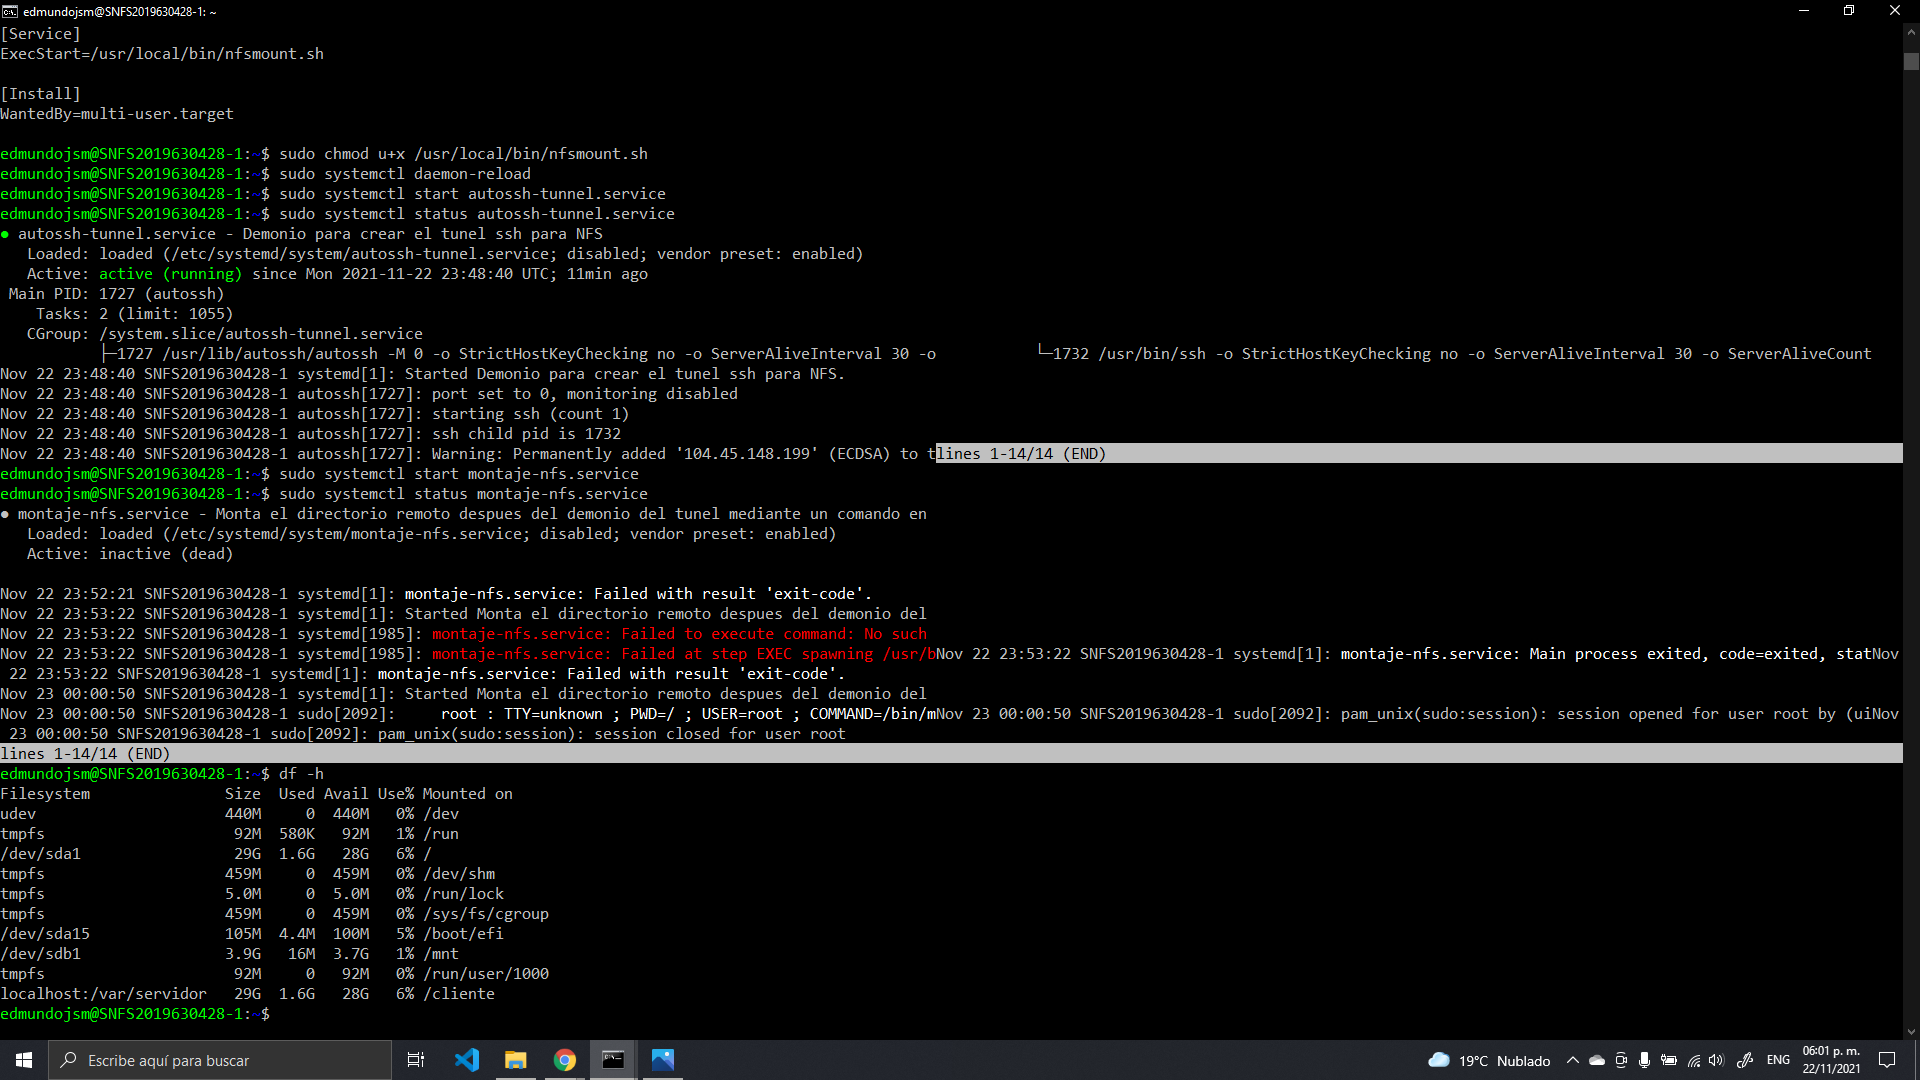
\includegraphics[scale=0.34]{resources/demoniosonc1.png}
			\caption{Demonios ejecutados de manera correcta.}\label{fig:picture}
		\end{figure}
		\subsubsection{Creación de los demonios en el cliente 2 }
		\begin{figure}[H]
			\centering
			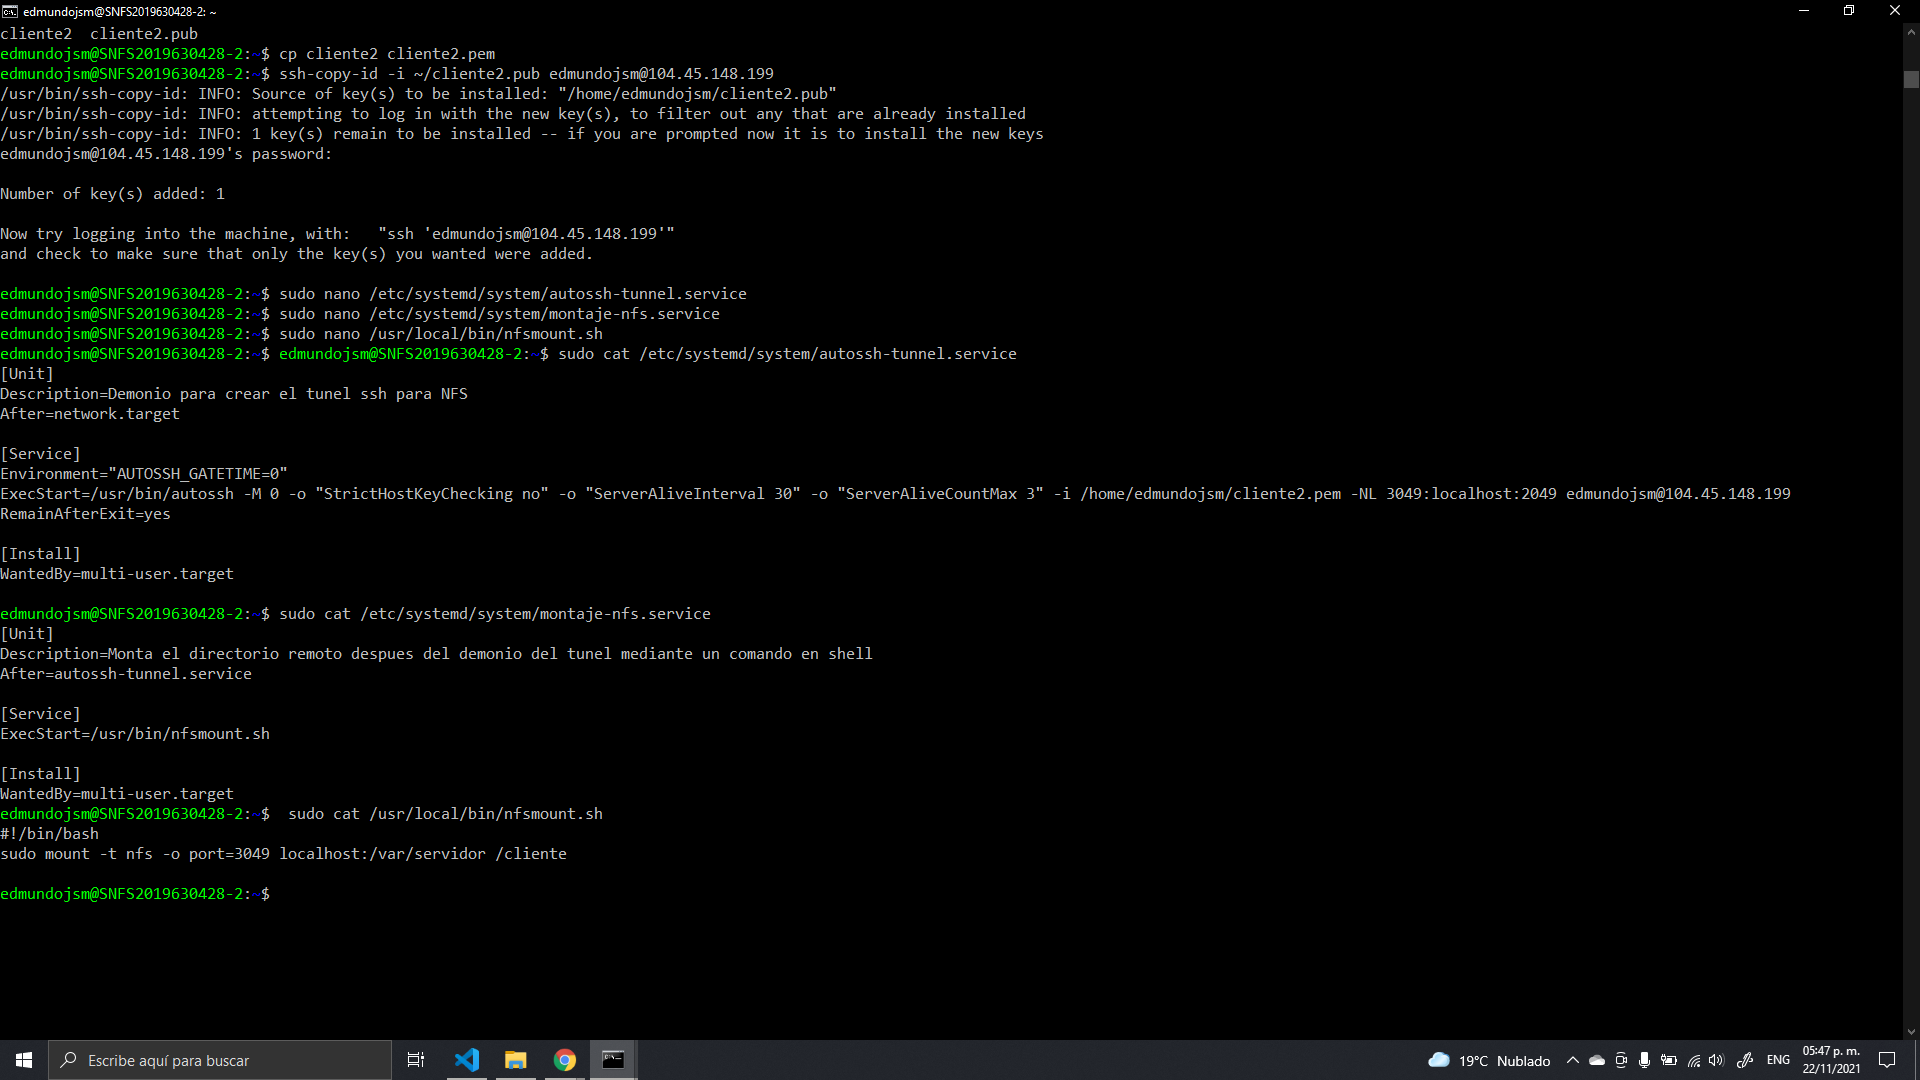
\includegraphics[scale=0.34]{resources/demonioc2.png}
			\caption{Creación de demonio y script en shell para el cliente 2.}\label{fig:picture}
		\end{figure}
		\begin{figure}[H]
			\centering
			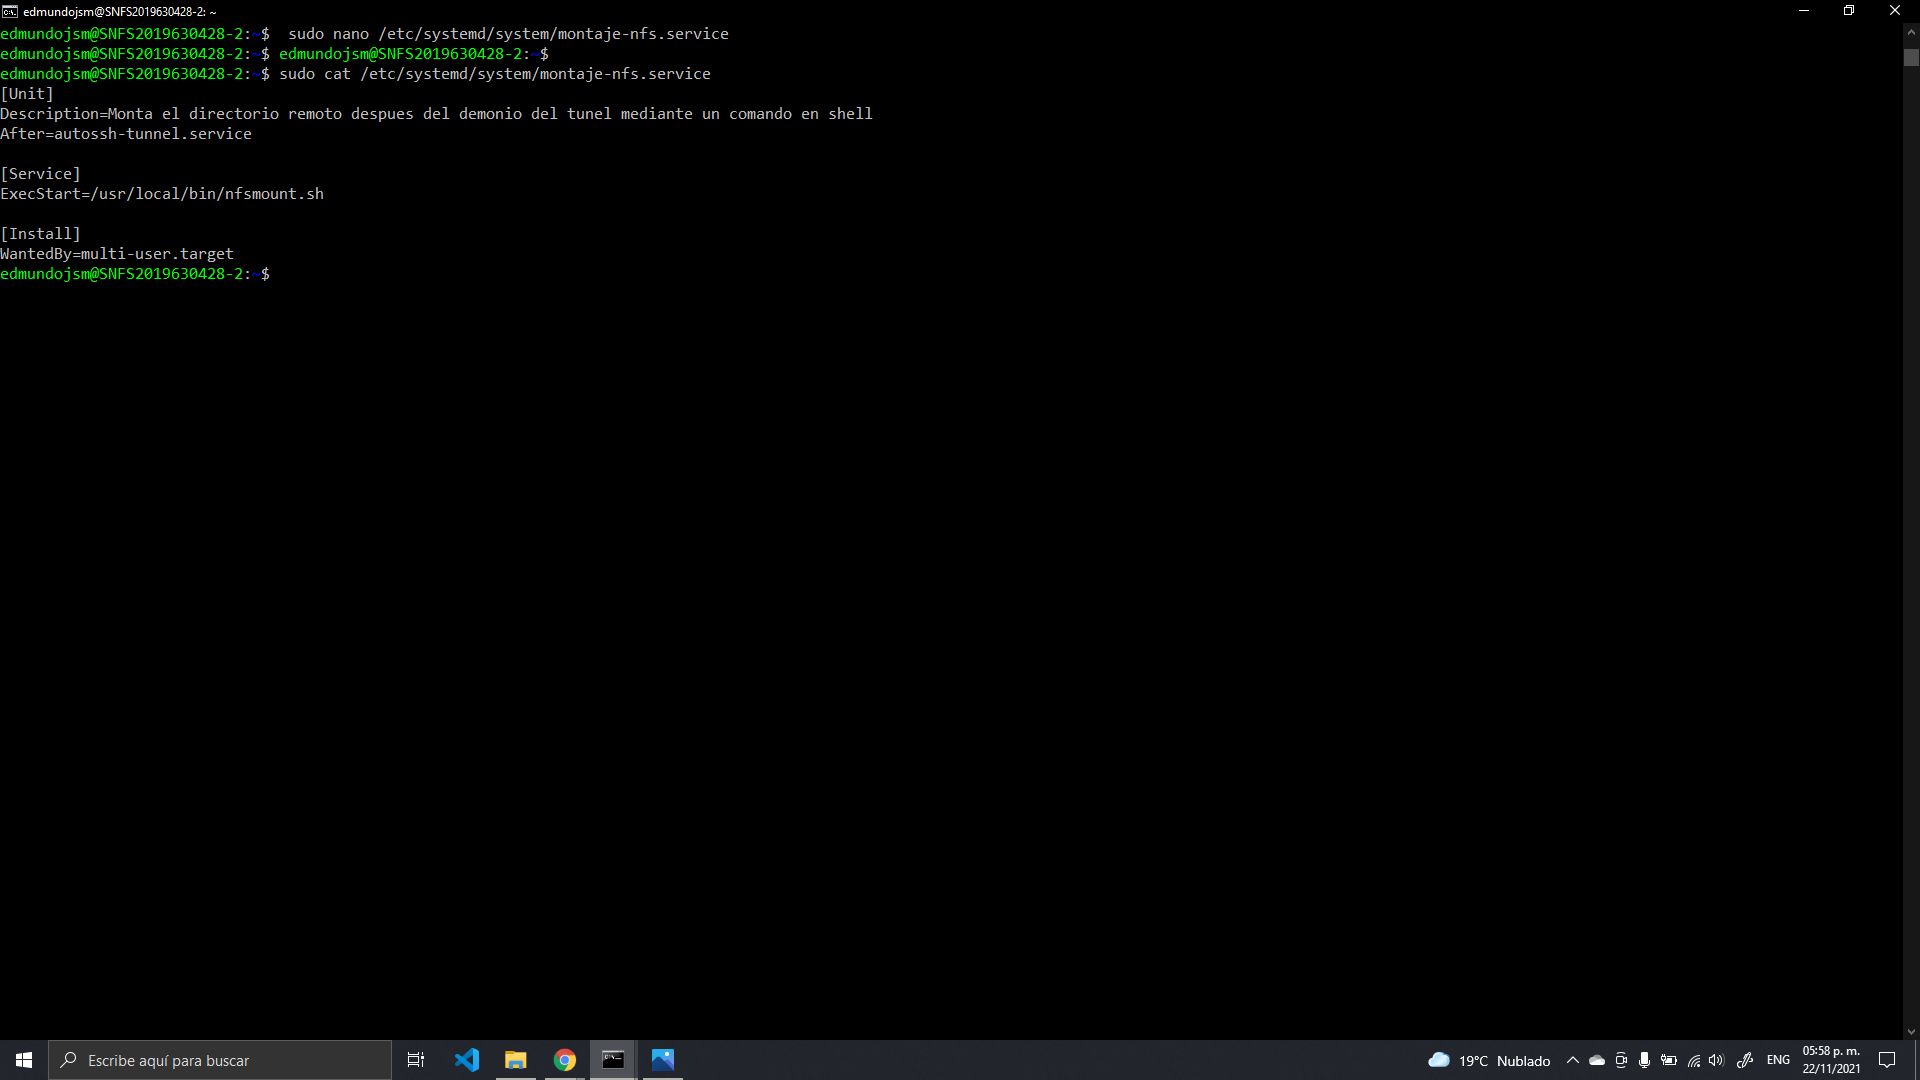
\includegraphics[scale=0.34]{resources/demonioc2actu.png}
			\caption{Actualización en la ruta del script en shell.}\label{fig:picture}
		\end{figure}
		 \begin{figure}[H]
			\centering
			\includegraphics[scale=0.34]{resources/demoniosonc2.png}
			\caption{Demonios ejecutados de manera correcta.}\label{fig:picture}
		\end{figure}
		
		\subsection{Configuración de los demonios para iniciar en el boot del sistema (ambos clientes)}
		En esta parte veremos la configuración de los demonios para que inicien justo después del boot del sistema y vemos como hacemos un reboot de ambos clientes, se puso fuera del apartado anterior ya que es parte del procedimiento, mencionar que necesitamos hace sudo systemctl start ``nombre de demonio'' y después sudo systemctl enable ``nombre de demonio'' para que estos empiecen desde el boot, en caso contrario no funcionaran desde el boot.
		\begin{figure}[H]
			\centering
			\includegraphics[scale=0.34]{resources/p8y9c1.png}
			\caption{Reboot y demonios inician desde el boot cliente 1.}\label{fig:picture}
		\end{figure}
		\begin{figure}[H]
			\centering
			\includegraphics[scale=0.34]{resources/p8y9c2.png}
			\caption{Reboot y demonios inician desde el boot cliente 2.}\label{fig:picture}
		\end{figure}	
			
		\subsection{En el cliente 1 desplegar el archivo /cliente/archivo.txt utilizando el comando ``more''}
		En esta parte veremos el desplegado del archivo creado en pasos anteriores justo después de ingresar al sistema.
		\begin{figure}[H]
			\centering
			\includegraphics[scale=0.34]{resources/p10.png}
			\caption{Contenido del archivo /cliente/archivo.txt en cliente 1.}\label{fig:picture}
		\end{figure}	
		\subsection{En el cliente 2 desplegar el archivo /cliente/archivo.txt utilizando el comando ``more''}
		En esta parte veremos el desplegado del archivo creado en pasos anteriores justo después de ingresar al sistema.
		\begin{figure}[H]
			\centering
			\includegraphics[scale=0.34]{resources/p11.png}
			\caption{Contenido del archivo /cliente/archivo.txt en cliente 2.}\label{fig:picture}
		\end{figure}	
		\subsection{En el cliente 2 modificar el archivo /cliente/archivo.txt, agregar al archivo el siguiente texto: ``estamos agregando texto al archivo''}
		En esta parte veremos como se agrega texto al archivo de prueba y vemos su contenido acutal en el cliente 2 mediante los comandos more y cat.
		\begin{figure}[H]
			\centering
			\includegraphics[scale=0.34]{resources/p12.png}
			\caption{Modificación del archivo /cliente/archivo.txt en cliente 2.}\label{fig:picture}
		\end{figure}
		\subsection{En el cliente 1 desplegar el archivo /cliente/archivo.txt utilizando el comando ``more''}
		En esta parte veremos como se desplega el archivo de prueba mediante el comando more.
		\begin{figure}[H]
			\centering
			\includegraphics[scale=0.34]{resources/p13.png}
			\caption{Desplegado del archivo /cliente/archivo.txt en cliente 1 con more.}\label{fig:picture}
		\end{figure}
		\subsection{En el cliente 1 eliminar el archivo /cliente/archivo.txt utilizando el comando ``rm'' y desplegado del contenido del directorio /cliente utilizando el comando ``ls''}
		En esta parte veremos como se elimina el archivo de prueba mediante el comando rm y ademas vemos el contenido del directorio /cliente en cliente 1 y veremos como este esta vació.
		\begin{figure}[H]
			\centering
			\includegraphics[scale=0.34]{resources/p14y15.png}
			\caption{Eliminación del archivo /cliente/archivo.txt en cliente 1 con rm.}\label{fig:picture}
		\end{figure}
		\subsection{En el cliente 2 desplegar el contenido del directorio /cliente utilizando el comando ``ls''}
		En esta parte veremos el contenido del directorio /cliente en cliente 2 y veremos como este esta vació.
		\begin{figure}[H]
			\centering
			\includegraphics[scale=0.34]{resources/p16.png}
			\caption{Contenido de la carpeta /cliente en cliente 2 con ls.}\label{fig:picture}
		\end{figure}
	\section{Extras}
		En estas ultimas dos imágenes podemos ver el status de los dos demonios creados y como estos iniciaron desde el momento de que se prendió la maquina virtual, por lo que podemos decir que la tarea fue realizada con éxito.
		\begin{figure}[H]
			\centering
			\includegraphics[scale=0.34]{resources/extrac1.png}
			\caption{Estatus de los 2 demonios en cliente 1.}\label{fig:picture}
		\end{figure}
		\begin{figure}[H]
			\centering
			\includegraphics[scale=0.34]{resources/extrac2.png}
			\caption{Estatus de los 2 demonios en cliente 2.}\label{fig:picture}
		\end{figure}
		\section{Conclusiones}
	En esta practica pudimos ver el uso de NFS media un puente SSH ya que por si solo NFS no ofrece una comunicación segura, caso contrario que el túnel SSH si ofrece, ademas vemos como el NFS se comporte a todos los clientes que estén conectados al servidor y como esto hace que todos los clientes pueden modificar archivos y que se actualicen en todos los clientes al mismo tiempo, esto seria útil para una empresa que tengan que modificar diversos archivos al mismo tiempo y que todos estén actualizados al mismo tiempo. Finalmente vemos como el uso de demonios nos permite automatizar procesos que tendríamos que hacer cada vez que quisiéramos conectarnos al servicio NFS esto claro que esto no se enseña en esta unidad de aprendizaje pero podemos ver como esta unidad de aprendizaje es integradora y que por algo esta seriada como de las ultimas materias.
		\begin{thebibliography}{1}
 \bibitem[label1]{cite_key1} Binaria. 2020. Cómo configurar un punto de montaje NFS en Ubuntu 20.04. [online] Available at: https://www.blog.binaria.uno/2020/05/19/como-configurar-un-punto-de-montaje-nfs-en-ubuntu-20-04/ [Accessed 23 November 2021].
  \bibitem[label1]{cite_key1}Beginninglinux.com. 2008. Authentication without password using OpenSSH Key, certificates .pem and .pub - BeginningLinux.com. [online] Available at: http://www.beginninglinux.com/home/server-administration/openssh-keys-certificates-authentication-pem-pub-crt [Accessed 23 November 2021].
   \bibitem[label1]{cite_key1} Qastack.mx. 2018. ¿Cómo mantener confiablemente abierto un túnel SSH?. [online] Available at: https://qastack.mx/superuser/37738/how-to-reliably-keep-an-ssh-tunnel-open [Accessed 23 November 2021].
   \bibitem[label1]{cite_key1} startup, S. and Udosen, G., 2017. Start autossh on system startup. [online] Ask Ubuntu. Available at: https://askubuntu.com/questions/947841/start-autossh-on-system-startup [Accessed 23 November 2021].
   \bibitem[label1]{cite_key1} Stack Overflow. 2014. Start systemd service after specific service?. [online] Stack Overflow. Available at: https://stackoverflow.com/questions/21830670/start-systemd-service-after-specific-service [Accessed 23 November 2021].
   \bibitem[label1]{cite_key1}  Stack Overflow. 2019. why am I getting Exec format error when I am writing my linux service?. [online] Available at: https://stackoverflow.com/questions/57025605/why-am-i-getting-exec-format-error-when-i-am-writing-my-linux-service [Accessed 23 November 2021].
\end{thebibliography}
\end{document}
